% Options for packages loaded elsewhere
\PassOptionsToPackage{unicode}{hyperref}
\PassOptionsToPackage{hyphens}{url}
\PassOptionsToPackage{dvipsnames,svgnames,x11names}{xcolor}
%
\documentclass[
  letterpaper,
  DIV=11,
  numbers=noendperiod]{scrreprt}

\usepackage{amsmath,amssymb}
\usepackage{iftex}
\ifPDFTeX
  \usepackage[T1]{fontenc}
  \usepackage[utf8]{inputenc}
  \usepackage{textcomp} % provide euro and other symbols
\else % if luatex or xetex
  \usepackage{unicode-math}
  \defaultfontfeatures{Scale=MatchLowercase}
  \defaultfontfeatures[\rmfamily]{Ligatures=TeX,Scale=1}
\fi
\usepackage{lmodern}
\ifPDFTeX\else  
    % xetex/luatex font selection
\fi
% Use upquote if available, for straight quotes in verbatim environments
\IfFileExists{upquote.sty}{\usepackage{upquote}}{}
\IfFileExists{microtype.sty}{% use microtype if available
  \usepackage[]{microtype}
  \UseMicrotypeSet[protrusion]{basicmath} % disable protrusion for tt fonts
}{}
\makeatletter
\@ifundefined{KOMAClassName}{% if non-KOMA class
  \IfFileExists{parskip.sty}{%
    \usepackage{parskip}
  }{% else
    \setlength{\parindent}{0pt}
    \setlength{\parskip}{6pt plus 2pt minus 1pt}}
}{% if KOMA class
  \KOMAoptions{parskip=half}}
\makeatother
\usepackage{xcolor}
\setlength{\emergencystretch}{3em} % prevent overfull lines
\setcounter{secnumdepth}{5}
% Make \paragraph and \subparagraph free-standing
\ifx\paragraph\undefined\else
  \let\oldparagraph\paragraph
  \renewcommand{\paragraph}[1]{\oldparagraph{#1}\mbox{}}
\fi
\ifx\subparagraph\undefined\else
  \let\oldsubparagraph\subparagraph
  \renewcommand{\subparagraph}[1]{\oldsubparagraph{#1}\mbox{}}
\fi


\providecommand{\tightlist}{%
  \setlength{\itemsep}{0pt}\setlength{\parskip}{0pt}}\usepackage{longtable,booktabs,array}
\usepackage{calc} % for calculating minipage widths
% Correct order of tables after \paragraph or \subparagraph
\usepackage{etoolbox}
\makeatletter
\patchcmd\longtable{\par}{\if@noskipsec\mbox{}\fi\par}{}{}
\makeatother
% Allow footnotes in longtable head/foot
\IfFileExists{footnotehyper.sty}{\usepackage{footnotehyper}}{\usepackage{footnote}}
\makesavenoteenv{longtable}
\usepackage{graphicx}
\makeatletter
\def\maxwidth{\ifdim\Gin@nat@width>\linewidth\linewidth\else\Gin@nat@width\fi}
\def\maxheight{\ifdim\Gin@nat@height>\textheight\textheight\else\Gin@nat@height\fi}
\makeatother
% Scale images if necessary, so that they will not overflow the page
% margins by default, and it is still possible to overwrite the defaults
% using explicit options in \includegraphics[width, height, ...]{}
\setkeys{Gin}{width=\maxwidth,height=\maxheight,keepaspectratio}
% Set default figure placement to htbp
\makeatletter
\def\fps@figure{htbp}
\makeatother
% definitions for citeproc citations
\NewDocumentCommand\citeproctext{}{}
\NewDocumentCommand\citeproc{mm}{%
  \begingroup\def\citeproctext{#2}\cite{#1}\endgroup}
\makeatletter
 % allow citations to break across lines
 \let\@cite@ofmt\@firstofone
 % avoid brackets around text for \cite:
 \def\@biblabel#1{}
 \def\@cite#1#2{{#1\if@tempswa , #2\fi}}
\makeatother
\newlength{\cslhangindent}
\setlength{\cslhangindent}{1.5em}
\newlength{\csllabelwidth}
\setlength{\csllabelwidth}{3em}
\newenvironment{CSLReferences}[2] % #1 hanging-indent, #2 entry-spacing
 {\begin{list}{}{%
  \setlength{\itemindent}{0pt}
  \setlength{\leftmargin}{0pt}
  \setlength{\parsep}{0pt}
  % turn on hanging indent if param 1 is 1
  \ifodd #1
   \setlength{\leftmargin}{\cslhangindent}
   \setlength{\itemindent}{-1\cslhangindent}
  \fi
  % set entry spacing
  \setlength{\itemsep}{#2\baselineskip}}}
 {\end{list}}
\usepackage{calc}
\newcommand{\CSLBlock}[1]{\hfill\break\parbox[t]{\linewidth}{\strut\ignorespaces#1\strut}}
\newcommand{\CSLLeftMargin}[1]{\parbox[t]{\csllabelwidth}{\strut#1\strut}}
\newcommand{\CSLRightInline}[1]{\parbox[t]{\linewidth - \csllabelwidth}{\strut#1\strut}}
\newcommand{\CSLIndent}[1]{\hspace{\cslhangindent}#1}

\KOMAoption{captions}{tableheading}
\makeatletter
\@ifpackageloaded{tcolorbox}{}{\usepackage[skins,breakable]{tcolorbox}}
\@ifpackageloaded{fontawesome5}{}{\usepackage{fontawesome5}}
\definecolor{quarto-callout-color}{HTML}{909090}
\definecolor{quarto-callout-note-color}{HTML}{0758E5}
\definecolor{quarto-callout-important-color}{HTML}{CC1914}
\definecolor{quarto-callout-warning-color}{HTML}{EB9113}
\definecolor{quarto-callout-tip-color}{HTML}{00A047}
\definecolor{quarto-callout-caution-color}{HTML}{FC5300}
\definecolor{quarto-callout-color-frame}{HTML}{acacac}
\definecolor{quarto-callout-note-color-frame}{HTML}{4582ec}
\definecolor{quarto-callout-important-color-frame}{HTML}{d9534f}
\definecolor{quarto-callout-warning-color-frame}{HTML}{f0ad4e}
\definecolor{quarto-callout-tip-color-frame}{HTML}{02b875}
\definecolor{quarto-callout-caution-color-frame}{HTML}{fd7e14}
\makeatother
\makeatletter
\@ifpackageloaded{bookmark}{}{\usepackage{bookmark}}
\makeatother
\makeatletter
\@ifpackageloaded{caption}{}{\usepackage{caption}}
\AtBeginDocument{%
\ifdefined\contentsname
  \renewcommand*\contentsname{Table of contents}
\else
  \newcommand\contentsname{Table of contents}
\fi
\ifdefined\listfigurename
  \renewcommand*\listfigurename{List of Figures}
\else
  \newcommand\listfigurename{List of Figures}
\fi
\ifdefined\listtablename
  \renewcommand*\listtablename{List of Tables}
\else
  \newcommand\listtablename{List of Tables}
\fi
\ifdefined\figurename
  \renewcommand*\figurename{Figure}
\else
  \newcommand\figurename{Figure}
\fi
\ifdefined\tablename
  \renewcommand*\tablename{Table}
\else
  \newcommand\tablename{Table}
\fi
}
\@ifpackageloaded{float}{}{\usepackage{float}}
\floatstyle{ruled}
\@ifundefined{c@chapter}{\newfloat{codelisting}{h}{lop}}{\newfloat{codelisting}{h}{lop}[chapter]}
\floatname{codelisting}{Listing}
\newcommand*\listoflistings{\listof{codelisting}{List of Listings}}
\makeatother
\makeatletter
\makeatother
\makeatletter
\@ifpackageloaded{caption}{}{\usepackage{caption}}
\@ifpackageloaded{subcaption}{}{\usepackage{subcaption}}
\makeatother
\ifLuaTeX
  \usepackage{selnolig}  % disable illegal ligatures
\fi
\usepackage{bookmark}

\IfFileExists{xurl.sty}{\usepackage{xurl}}{} % add URL line breaks if available
\urlstyle{same} % disable monospaced font for URLs
\hypersetup{
  pdftitle={HerbVar Project Manual \& Field Protocols},
  pdfauthor={The Herbvar Steering Committee},
  colorlinks=true,
  linkcolor={blue},
  filecolor={Maroon},
  citecolor={Blue},
  urlcolor={Blue},
  pdfcreator={LaTeX via pandoc}}

\title{HerbVar Project Manual \& Field Protocols}
\author{The Herbvar Steering Committee}
\date{2024-05-03}

\begin{document}
\maketitle

\renewcommand*\contentsname{Table of contents}
{
\hypersetup{linkcolor=}
\setcounter{tocdepth}{2}
\tableofcontents
}
\bookmarksetup{startatroot}

\chapter*{Preamble}\label{preamble}
\addcontentsline{toc}{chapter}{Preamble}

\markboth{Preamble}{Preamble}

This book is a manual for researchers involved the the
\href{https://herbvar.org/}{HerbVar Project}. It includes a checklist
for new collaborators, guidelines on accessing, adding, and using
project data, tutorials for using the RStudio Project Templates for
conducting analyses and preparing manuscripts, protocols for field work,
and guides for administering the HerbVar Network resources (\emph{e.g.,}
website, data portal).

This guide is a \href{https://quarto.org/docs/books}{Quarto Book} hosted
on the \href{https://github.com/HerbVar-Network}{HerbVar Network's
Github site}, so any team members can edit the text, add new sections,
or make suggestions for improvement either by
\href{https://github.com/HerbVar-Network/project_manual/pulls}{pull
request} or by
\href{https://github.com/HerbVar-Network/project_manual/issues}{posting
an issue} on the HerbVar Manual's repository. A tutorial on getting
started with Quarto and RStudio can be found
\href{https://quarto.org/docs/get-started/hello/rstudio.html}{here}.

\begin{center}\rule{0.5\linewidth}{0.5pt}\end{center}

\part{What is HerbVar?}

\chapter{HerbVar Overview}\label{sec-overview}

\section{Motivation}\label{motivation}

Published studies and personal observations suggest the distribution of
herbivore feeding damage among individual plants within a population is
often highly skewed such that most plants experience relatively low
levels of damage, and a small fraction of plants experience
disproportionately high levels of damage. Theory suggests that such
variability can have dramatic ecological and evolutionary consequences.
For example, variability among plants can lead overall herbivore
population size to be greater or less than expected based on average
plant quality and asymmetric fitness surfaces can lead to
over-investment in defensive traits. \textbf{\emph{Surprisingly, despite
the theoretical importance and potential generality of variability in
herbivory, it has received little empirical attention, limiting our
fundamental understanding of how plants and herbivores interact.}} We
are a global collaboration to quantify the distribution of herbivory for
diverse plant species in multiple ecosystems across the world.

\section{Objectives}\label{objectives}

\textbf{The goals of HerbVar are (1)} to assess if variability in
herbivory is indeed a common feature of plant--herbivore interactions,
and \textbf{(2)} to examine how the amount of variability and skew
varies among different types of plant species, herbivore communities,
and ecosystems. Quantifying general patterns in the distribution of
herbivore damage within populations would be a major contribution to our
fundamental understanding of herbivory. In addition, identifying the
factors that correlate with variability in herbivory would provide the
field with a new paradigm for describing plant--herbivore interactions
and allow us to generate novel hypotheses about the ecology and
evolution of plant--herbivore interactions. Among the factors under
consideration are:

\begin{itemize}
\tightlist
\item
  Plant species identity,
\item
  Plant functional traits (from literature),
\item
  Plant ecology (e.g., rarity),
\item
  Herbivore species,
\item
  Herbivore functional groups,
\item
  Ecosystem type,
\item
  Latitude,
\item
  \ldots and many others (e.g., seasonality, precipitation).
\end{itemize}

\section{Questions?}\label{questions}

More information on the HerbVar Project is available on the
\href{https://herbvar.org/}{project website}. If you can't find the
information you're looking for in this manual or the website, please
contact a member of the HerbVar Steering Committee:

\begin{itemize}
\tightlist
\item
  Nora Underwood
  \href{mailto:nunderwood@bio.fsu.edu}{\nolinkurl{nunderwood@bio.fsu.edu}}\\
\item
  Brian Inouye
  \href{mailto:binouye@bio.fsu.edu}{\nolinkurl{binouye@bio.fsu.edu}}\\
\item
  Susan Whitehead
  \href{mailto:swhitehead@vt.edu}{\nolinkurl{swhitehead@vt.edu}}\\
\item
  Phil Hahn \href{mailto:hahnp@ufl.edu}{\nolinkurl{hahnp@ufl.edu}}\\
\item
  Lee Dyer
  \href{mailto:nolaclimber@gmail.com}{\nolinkurl{nolaclimber@gmail.com}}\\
\item
  Emilio Bruna
  \href{mailto:embruna@ufl.edu}{\nolinkurl{embruna@ufl.edu}}\\
\item
  Ivalu Cacho
  \href{mailto:ivalu.cacho@gmail.com}{\nolinkurl{ivalu.cacho@gmail.com}}\\
\item
  Karen Abbott
  \href{mailto:kca27@case.edu}{\nolinkurl{kca27@case.edu}}\\
\item
  Will Wetzel
  \href{mailto:william.wetzel@montana.edu}{\nolinkurl{william.wetzel@montana.edu}}
\end{itemize}

\part{New Collaborators: Start Here}

\chapter{First Steps}\label{first-steps}

\begin{enumerate}
\def\labelenumi{\arabic{enumi}.}
\tightlist
\item
  Add info to Collaborator Contact Information file
\end{enumerate}

\begin{itemize}
\tightlist
\item
  make sure you have:

  \begin{itemize}
  \tightlist
  \item
    orcid id
  \item
    github account
  \end{itemize}
\end{itemize}

\begin{enumerate}
\def\labelenumi{\arabic{enumi}.}
\tightlist
\item
  Get added as ``Contributor'' to the HerbVar Shared Drive (see if this
  is still best way)
\item
  get added to slack
\item
  get added to herbvar zotero group
\item
  request access to github
\item
  Review Authorship Guidelines
\item
  Sign Data Use Agreement
\end{enumerate}

\chapter{Collaborator Agreement}\label{collaborator-agreement}

\chapter{Proposing New Analyses}\label{proposing-new-analyses}

\section{Working Group Projects}\label{working-group-projects}

\section{Add-on Projects}\label{add-on-projects}

\chapter{Becoming a Site PI}\label{becoming-a-site-pi}

\part{Research Workflow}

\chapter{HerbVar Workflow Overview}\label{sec-workflow}

HerbVar relies heavily on version control with Git/Github to facilitate
data validation and management (Goodman et al. 2014, Yenni et al. 2019,
Kim et al. 2022), promote collaboration (Boland et al. 2017, Braga et
al. 2023), and streamline data access, analysis, and archiving
(Champieux et al. 2023). Below we describe the workflow for (a)
collecting data for HerbVar and uploading it for integration with the
global data set and (b) analyzing some or all of the global HerbVar data
set and preparing a manuscript based on these analyses.

\section{Collecting new HerbVar Data}\label{collecting-new-herbvar-data}

\begin{enumerate}
\def\labelenumi{\arabic{enumi}.}
\tightlist
\item
  Review and Select Protocols
\item
  Collect Data
\item
  Create a repository for cleaning the data using the
  \texttt{new\_dataset\_template}.
\item
  Upload the clean version of the data using the portal
\end{enumerate}

\section{New analysis with Herbvar
Datasets}\label{new-analysis-with-herbvar-datasets}

\begin{enumerate}
\def\labelenumi{\arabic{enumi}.}
\tightlist
\item
  Identify Questions, Submit for Review to make sure no overlap
\item
  Create a repository for harvesting, organizing, and analyzing the data
  to be used in the analyses using the
  \texttt{new\_analysis\_and\_paper\_template}.
\item
  This template can also be used to write the manuscript in markfdown
  using a template such as \texttt{papaja} or one of the 'rticles`
  templates.
\end{enumerate}

\chapter{Data Collection Protocols}\label{sec-data-collection}

\begin{tcolorbox}[enhanced jigsaw, opacityback=0, colback=white, breakable, toprule=.15mm, title=\textcolor{quarto-callout-important-color}{\faExclamation}\hspace{0.5em}{Important}, left=2mm, coltitle=black, bottomrule=.15mm, arc=.35mm, leftrule=.75mm, rightrule=.15mm, bottomtitle=1mm, toptitle=1mm, colframe=quarto-callout-important-color-frame, colbacktitle=quarto-callout-important-color!10!white, opacitybacktitle=0.6, titlerule=0mm]

Below are links to the HerbVar sampling protocols. Please be sure to
review the larger strategic vision and project goals of the HerbVar
Network, which are summarized in Chapter~\ref{sec-overview}.

\end{tcolorbox}

\section{Species \& site selection}\label{species-site-selection}

Our approach to select plant species and/or sites to survey is described
in Chapter~\ref{sec-species_site}. Briefly, we suggest collaborators
strive to survey either:

\begin{enumerate}
\def\labelenumi{(\arabic{enumi})}
\tightlist
\item
  One of our three focal species -- \emph{Taraxacum officinale},
  \emph{Plantago lanceolata}, and \emph{Plantago major} -- in a novel
  geographic/environmental context\\
\item
  New clades or growth forms of species in our five focal families:
  Apocynaceae, Asteraceae, Fabaceae, Rubiaceae, and Solanaceae, or\\
\item
  Reproductive tissue damage of any species.
\end{enumerate}

\section{Primary Protocol}\label{primary-protocol}

The \textbf{Primary Protocol} for collecting HerbVar data with most
species (e.g., sample sizes, selecting individuals to sample) is
described in Chapter~\ref{sec-primary}. If there is a reason why you
think this protocol will not work for your species or in your field
sites, please consider one of the alternative protocols below or contact
the HerbVar Planning Group.

\textbf{Estimating damage by herbivores}: Chapter~\ref{sec-damage}
provides a detailed walk-through of the process for estimating herbivore
damage on leaves and whole plants, including suggestions for different
types of leaves and damage. There is also an
\href{./protocols/Illustrated\%20Guide\%20to\%20Percent\%20Leaf\%20Damage.pdf}{Illustrated
Guide to Percent Leaf Damage} to help estimate different levels of to
damage to leaves. \emph{We suggest printing this guide and taking it
with you to the field to help estimate percent herbivory.} It currently
includes leaves of two species as examples, but it will be updated
periodically with examples from other species.

\begin{itemize}
\item
  \href{protocols/HerbVar_Datasheet_Template.xlsx}{Datasheet - Excel
  File}. This Excel file is a template datasheet designed to work for
  the HerbVar Primary Protocol. It contains a ``data dictionary'' sheet
  that defines all columns if any abbreviations are unclear.
\item
  \href{https://drive.google.com/drive/folders/10-9xPm9yOAvGCtL3dmVaoz7ODI1fghYG?usp=sharing}{Datasheet
  - Printable PDFs}. We have split the printable datasheets into three
  parts, one each for the Primary, Reproductive, and Herbivore
  Protocols. The herbivore datasheet is built for you to print as many
  copies of the second page as you have identified herbivore groups.
\end{itemize}

\section{Damage to reproductive
tissues}\label{damage-to-reproductive-tissues}

If your plants have reproductive tissues (e.g., flowers, fruits, seeds),
please follow the protocol in Chapter~\ref{sec-repro} to quantify damage
to these tissues.

\section{Alternative survey
protocols}\label{alternative-survey-protocols}

\begin{itemize}
\item
  \textbf{Rare Plants:} Chapter~\ref{sec-low_density} describes
  protocols for rare plants (i.e., plants found at low densities /
  abundances).
\item
  \textbf{Cacti \& Other Succulents:} Chapter~\ref{sec-succulents}
  describes protocols and issues related to quantifying herbivory on
  cacti and other succulents.
\item
  \textbf{Trees:} Chapter~\ref{sec-tree} is a protocol for surveying
  mature trees. It also discusses how to handle seedlings and saplings
  of tree species. If you are sampling tree species in their seedling or
  sapling stage (i.e., \textless2m tall) please refer to the Primary
  Protocol.
\item
  \textbf{Rhizomatous species:} Chapter~\ref{sec-rhizo} is a protocol
  for rhizomatous species for which it is feasible to determine what
  constitutes a genet (e.g., by identifying rhizomatous connections) and
  for which genets are small enough that herbivory could be estimated on
  \textasciitilde30 genets in a site and their nearest neighbors.
\end{itemize}

\section{Sampling Insects}\label{sampling-insects}

All surveys should note internally-feeding herbivores (e.g., gallers and
miners), but only some should take the extra time to sample external
herbivores. Chapter~\ref{sec-herbivore} discusses \emph{whether and how}
to sample insects, and includes visual cheatsheets for several
identifying several focal groups of insects and for counting galls and
mines.

\section{Entering and Correcting
Data}\label{entering-and-correcting-data}

\textbf{\emph{Do not make any changes to the raw data files once you
have entered the data.}} Make any corrections using R scripts. For
additional information on how to do this, see
Chapter~\ref{sec-data-analysis}

\chapter{Uploading Data}\label{uploading-data}

To upload data, please visit our
\href{https://herbvar.shinyapps.io/data_portal_actual/}{data submission
portal} and be sure to use the template Excel file linked in
Chapter~\ref{sec-data-collection}

\chapter{Data Analysis}\label{sec-data-analysis}

Instructions for using setting up a github repository for data analysis
and making reproducible corrections using scripts.

\chapter{Preparing HerbVar
Manuscripts}\label{preparing-herbvar-manuscripts}

Manuscript Preparation using the github repository / template

\section{Reproducible Manuscripts}\label{reproducible-manuscripts}

The same template for analyses can be used for creating a manuscript
with Rmd

\section{Prior to Submission}\label{prior-to-submission}

{[} {]} All HerbVar publications must include the following text in the
Acknowledgements:

``This work was supported by the National Science Foundation (Grant
No.~DEB-2203582).''

{[} {]} If the data set used has been archived at Dryad, please cite
both the data set and the original article in your paper section. For
example, include citations to both:

Wetzel, William et al.~(2023). Plant size, latitude, and phylogeny
explain within-population variability in herbivory {[}Dataset{]}. Dryad.
\url{https://doi.org/10.5061/dryad.44j0zpckm}

and

The Herbivory Variability Network. 2023. Plant size, latitude, and
phylogeny explain within-population variability in herbivory.
\emph{Science} 382: 679-683. \url{DOI:10.1126/science.adh8830}

\section{Following Submission}\label{following-submission}

{[} {]} Add the MS to the Zotero Group (Important for NSF reporting to
know how many manuscripts are in review.)

{[} {]} Post a Preprint (optional but encouraged)

\section{Upon Acceptance}\label{upon-acceptance}

{[} {]} Update the record in the Zotero library

{[} {]} Archive the Data with Dryad

\begin{itemize}
\tightlist
\item
  only if the data are new, otherwise MS will indicate data source as
  Dryad
\end{itemize}

{[} {]} Archive the Analysis Repo on Zenodo

\begin{itemize}
\tightlist
\item
  instructions on freezing the data analysis code repo on zenodo
\end{itemize}

{[} {]} Archive the Manuscript Repo on Zenodo (optional)

\begin{itemize}
\tightlist
\item
  instructions on freezing the MS repo on zenodo
\end{itemize}

\part{Protocols}

\chapter{Species \& Site Selection (Phase 2)}\label{sec-species_site}

Based on Phase 1 of data collection, we ask that you prioritize the
following three objectives in your site and species selections for Phase
2 of data collection:

\begin{enumerate}
\def\labelenumi{(\arabic{enumi})}
\tightlist
\item
  Sampling one of three focal species across gradients,\\
\item
  Sampling novel species \& contexts within focal families, and
\item
  Quantifying damage to reproductive tissues
\end{enumerate}

\section{Objective 1: Focal species across
gradients}\label{objective-1-focal-species-across-gradients}

\textbf{Goal: }Sample our three focal species -- \emph{Taraxacum
officinale}, \emph{Plantago major}, and \emph{Plantago lanceolata} --
across broad geographic and/or environmental gradients.

\textbf{Justification:} Sampling within these three species will
increase the depth of our understanding of the effects of particular
abiotic gradients (e.g., elevation, precipitation, temperature, etc.) as
drivers of variability in herbivory pressure within plant species. Each
species is standardized within itself so studies of herbivory across a
range of contexts allows for strong inference on the effects of those
contexts.

\section{Species Objective 2: Novel species \& contexts within focal
families}\label{species-objective-2-novel-species-contexts-within-focal-families}

\textbf{Goal: }Sample species from novel clades or with atypical growth
forms within our five focal families -- Apocynaceae, Asteraceae,
Fabaceae, Rubiaceae, and Solanaceae. Surveys of plant species that were
included in Phase 1 are also welcomed but should prioritize novel
regions, habitats, or environmental contexts.

\textbf{Justification:} Increased resolution within our five focal
families allows for testing of drivers of herbivory variability in a
phylogenetically-explicit framework. Understanding the impact of
evolutionary differences within these families on the distribution of
damage will be crucial in teasing apart macroevolutionary patterns.

\section{Species Objective 3: Damage to Reproductive
Tissues}\label{species-objective-3-damage-to-reproductive-tissues}

\textbf{Goal: }Survey damage to the fruits, flowers, and seeds of any
species.

\textbf{Justification:} Damage to reproductive structures
has--arguably--the most direct impact on fitness so an understanding of
the drivers of variation in herbivory damage to reproductive tissues is
crucial for understanding population-level or fecundity-related
consequences of herbivory variation.

\section{Site Selection Guidelines}\label{site-selection-guidelines}

\textbf{Goal:} A ``site'' should be an area where a given plant species
occurs at a high enough density to easily select 30 focal plants and 30
unique neighbors with our method. We can use any site anywhere around
the world, but the most valuable sites will represent geographic
regions, environmental conditions, habitats, or other ecological
characteristics that we do not currently have in our database or that
are currently poorly represented in our database. This is especially
important for our focal species and re-surveys of other species we
already have in our database. It's less important for new species,
especially when those new species are from clades that we do not
currently have in the database.

\textbf{Further Explanation:} We realize that defining the `edges' of a
site can be subjective and not easy. Walk around and see if you see the
density drop off to well below the mean density that is used to
calculate radius size (see Chapter~\ref{sec-primary}). This is usually
quite simple; for example, when we walk out from the center of a
``site'' and don't see any individuals of the focal species within 5 m,
we decide we're at the edge of a patch. In some systems, delineating a
single, population that can be sampled simply might not be possible
(e.g., where a species covers a vast area). In these cases,
collaborators should simply do their best to select a reasonable,
representative area to sample.

\chapter{Primary Protocol}\label{sec-primary}

\begin{itemize}
\tightlist
\item
  TODO: add links to Below the Field \#3 below
\end{itemize}

Below, we provide a straight-forward and broadly applicable protocol to
achieve project goal of quantifying variability in plant-herbivore
interactions. This is HerbVar's Primary Survey Protocol. In brief, 30
randomly selected plant individuals in a site
(\textasciitilde population) are surveyed for herbivore damage and
(possibly) herbivore abundance. Data are also collected on the nearest
conspecific neighbor of each plant (for a total of N = 60 plants). These
methods yield estimates of variability, skew, and spatial patterns
(e.g., autocorrelation) in herbivore damage. For more information on the
broader motivations and goals of the project see here.

\textbf{Note on Alternate Protocols:} The HerbVar Primary Survey
Protocol is designed to work for many common plant growth forms and
contexts, so we expect most surveys to use this protocol. The primary
protocol, however, will not work for every plant growth form or context,
so HerbVar has multiple alternative survey protocols. These include
protocols for surveying the following:

\begin{itemize}
\tightlist
\item
  Reproductive damage: Chapter~\ref{sec-repro}
\item
  Low density/abundance populations: Chapter~\ref{sec-low_density}
\item
  Cacti and other succulents: Chapter~\ref{sec-succulents}
\item
  Mature trees: Chapter~\ref{sec-tree} \emph{(surveys of immature trees
  (i.e., seedling/saplings) use the Primary Protocol below)}
\item
  Rhizomatous geophytes: Chapter~\ref{sec-rhizo}
\item
  Insect herbivores, galls, and mines: Chapter~\ref{sec-herbivore}
\end{itemize}

If the primary protocol is not feasible for a species or site, then we
suggest one of these alternative protocols. If none of these alternative
protocols fits the situation, then collaborators may deviate from the
primary protocol. We trust collaborators to decide how to adapt the
primary protocol in ways that work for their systems. We suggest,
however, that collaborators strive to follow the spirit of the protocol
below: randomly select at least 30 plants from a site and census them
and their nearest neighbors for herbivory and herbivore data. For a
dataset to be usable in the overall study, it will have to be comparable
to data collected using this protocol. Collaborators who deviate from
the HerbVar protocols should carefully record their methods.

\section{Guidelines for Picking Plant
Species}\label{guidelines-for-picking-plant-species}

\subsection{Ideal Focal Species
Abundance}\label{ideal-focal-species-abundance}

The primary protocol works best for sites with at least
\textasciitilde90 plant individuals, such that it makes sense to sample
individuals randomly. If your site has fewer than \textasciitilde90
individuals of your plant species, then please consider comprehensively
censusing all individuals within the site as suggested in the Low
Density/Abundance Protocol. A comprehensive census, when feasible, would
be even better than the protocol below. If plants are far enough apart,
please take GPS coordinates for each plant. If a comprehensive census is
not feasible, then please modify the primary protocol or the
low-density/low-abundance guidelines to work efficiently with your
species and site. Please reach out to the HerbVar coordinators if you
have questions or want to check that your modifications will lead to
adequate data.

\subsection{Before the Field}\label{before-the-field}

\begin{enumerate}
\def\labelenumi{\arabic{enumi}.}
\item
  \textbf{Please review HerbVar's Damage Estimation Training Guidelines
  in Chapter~\ref{sec-damage}.} Note that information on precision of
  estimates and acceptable binning is contained in this document This
  document contains valuable information on how to estimate percent
  damage on various leaves.\\
\item
  \textbf{Please spend some time training and testing yourself and
  anyone working with you in the field using the
  \href{https://zaxherbivorytrainer.com/}{ZAX Herbivory Trainer}}. This
  web-based application, created by Dr.~Angela Moles and Zoe Xirocostas,
  provide a risk-free environment for testing oneself on per-leaf damage
  estimation Note that the app prompts you to assess damage to the
  nearest percent while our protocol is slightly coarser (see Table 1 of
  the Damage Estimation Guidelines). The app has two stages, one in
  which you assess damage and are immediately told how close you are to
  correct and a second where you assess 50 leaves, and the results are
  given to you at the end. Please feel free to focus on the first part
  of the app until you are confident (though you are of course welcome
  to do the second if you want extra training).
\item
  \textbf{Download the template datasheet for this protocol}. There are
  both digital (see siteData, densityData, and plantData sheets) and
  printable versions to facilitate standardized data entry. If you have
  a question on this, please feel free to reach out to
  \href{mailto:herbvar@gmail.com}{\nolinkurl{herbvar@gmail.com}}
\end{enumerate}

\section{Primary Protocol}\label{primary-protocol-1}

\begin{enumerate}
\def\labelenumi{\arabic{enumi}.}
\item
  Pick a plant species (see ``Guidelines for Selecting Plant Species''
  below)
\item
  Pick a site (see ``Delineating a Site'' below for advice)
\item
  Pick a time to sample (see ``When to Sample'' below for advice)
\item
  Determine a radius for your circular quadrats

  \begin{enumerate}
  \def\labelenumii{\alph{enumii}.}
  \item
    \textbf{If you are sampling one of the HerbVar focal species}
    (\emph{Taraxacum officinale, Plantago major, Plantago lanceolata}):
    Use a radius of 0.4 m for your quadrats. This will standardize
    across surveys of these same species. Note that if your populations
    are sparse, you may use a larger radius following the other process
    or pre-calculated values (Table 1).
  \item
    \textbf{If you are using any other species}, use the following
    process to determine a quadrat radius or use the table below:

    \begin{enumerate}
    \def\labelenumiii{\arabic{enumiii}.}
    \tightlist
    \item
      Estimate mean density of plant/1 m\(^2\)
    \item
      Count the number of plants in 1 m\(^2\) at 10 random locations
      within the site
    \item
      Calculate mean density (\emph{D})
    \item
      Use \emph{D} to calculate a circular quadrat radius (\emph{r})
      that would on average contain 4 plants \emph{r} = 4/(π\emph{D}).
    \item
      This approach seeks an optimal, intermediate quadrat size that
      balances the costs associated with a small quadrat size (many
      empty quadrats) and a large quadrat size (quadrats that require
      counting many plant individuals).
    \end{enumerate}
  \end{enumerate}
\end{enumerate}

Rather than calculating, you may also use this pre-calculated set of
radii (Table 1) for non-focal species. \textbf{\emph{Remember, for focal
species, please use 0.4 m}}

\begin{longtable}[]{@{}ll@{}}
\caption{Table 1. Pre-Calculated Quadrat Radii}\tabularnewline
\toprule\noalign{}
\textbf{Number plants/m2 (Density D)} & \textbf{Quadrat radius
(}r\textbf{)} \\
\midrule\noalign{}
\endfirsthead
\toprule\noalign{}
\textbf{Number plants/m2 (Density D)} & \textbf{Quadrat radius
(}r\textbf{)} \\
\midrule\noalign{}
\endhead
\bottomrule\noalign{}
\endlastfoot
D ≤ 0.1 & 3.6 meters \\
0.1 \textless{} D ≤ 0.25 & 2.9 m \\
0.25 \textless{} D ≤ 0.5 & 1.9 m \\
0.5 \textless{} D ≤ 1 & 1.35 m \\
1 \textless{} D ≤ 3 & 0.9 m \\
3 \textless{} D ≤ 6 & 0.55 m \\
6 \textless{} D ≤ 10 & 0.4 m \\
10 \textless{} D ≤ 20 & 0.3 m \\
20 \textless{} D & 0.23 m \\
\end{longtable}

\begin{enumerate}
\def\labelenumi{\arabic{enumi}.}
\setcounter{enumi}{4}
\item
  Lay a transect through the middle of the site (Fig. 1) Record GPS
  coordinates of origin, length (m), and compass direction (degrees) of
  transect (need to pick a coordinate system and precision)
\item
  Select center points of circular quadrats (Fig. 1). Randomly select
  40+ points in the site by selecting pairs of random numbers. One
  random number represents distance along the transect (0--length of
  transect); the other represents distance left or right of the transect
  (left=negative, 0=center, right=positive). These are the center points
  of quadrats.
\item
  For each quadrat:

  \begin{enumerate}
  \def\labelenumii{\alph{enumii}.}
  \item
    Locate a quadrat center point using transect and measuring tape or
    stick (Fig. 1)
  \item
    Count and record the number of focal plants within r meters of the
    center point (Fig. 1).
  \item
    See above for explanation of how to calculate r(or use values in
    Table 1).
  \end{enumerate}

  \begin{enumerate}
  \def\labelenumii{\roman{enumii}.}
  \setcounter{enumii}{1}
  \item
    It may be helpful to place a stick vertically in the center of the
    quadrat, attach a string of r meters to the tip, and walk in a
    circle around the stick to help visualize the circular quadrat
  \item
    \textbf{Note:} this includes only rooted focal plant species
    individuals in the quadrat
  \end{enumerate}
\item
  Record other quadrat-level data

  \begin{enumerate}
  \def\labelenumii{\alph{enumii}.}
  \item
    Percent cover of focal plant species (ignore non-focal species).
    \textbf{Note:} this includes both rooted and not rooted focal plant
    species individuals in the quadrat but hanging over the edge from
    above
  \item
    Percent cover of all non-focal plant species (ignore focal species)
  \item
    These 2 percent covers could total more than 100\% if they overlap
  \end{enumerate}

  \begin{enumerate}
  \def\labelenumii{\roman{enumii}.}
  \setcounter{enumii}{1}
  \tightlist
  \item
    If surveying understory plants, ignore forest canopy when estimating
    percent cover
  \end{enumerate}
\item
  If the circular quadrat has 0 plants, record a zero and continue to
  the next quadrat
\item
  If the circular quadrat has \textgreater{} 0 plants: Randomly choose 1
  of the plants within the quadrat to survey A quicker alternative would
  be to choose the plant closest to the quadrat center. But this is
  recommended only if you think it will produce an unbiased sample of
  plants from your site. Be careful about over-representing large and/or
  isolated plants (which will be closer to more points relative to small
  plants in crowded patches).
\item
  For the selected plant (1 per quadrat) record plant life stage I.e.,
  seedling, vegetative, flowering, fruiting Note that if multiple stages
  are present, record all relevant stages (i.e., a plant can be both
  flowering and fruiting)
\item
  For the selected plant record plant size. Use judgment to pick best
  measure for your species E.g., standing plant height (ground to
  tallest living part), stem length, foliage diameter, stem diameter
\item
  Perhaps most importantly: for the selected plant record herbivore
  damage in 3 ways (see Damage Estimation Training Guidelines) Note that
  ``herbivore damage'' includes damage caused by both vertebrate and
  invertebrate herbivores.
\end{enumerate}

\begin{enumerate}
\def\labelenumi{\alph{enumi}.}
\item
  Presence/absence of leaf damage: Record both (A) the total number of
  leaves on the plant and (B) the number of leaves with
  \textgreater0.5\% herbivory

  \begin{enumerate}
  \def\labelenumii{\roman{enumii}.}
  \item
    If the plant has ≤ 60 leaves total, please record the true numbers
  \item
    If the plant has \textgreater60 leaves total, randomly (arbitrarily)
    choose 60 and record those values. Please also make a note that you
    stopped at 60 (see template datasheet).
  \item
    Note that we are no longer including undamaged leaves in the
    following step, so these two data points are vital in understanding
    the proportion of the plant that is not damaged by herbivores.
  \item
    If plants have reproductive parts (flowers/fruits/seeds) that could
    have been damaged by herbivores, please see the Reproductive Damage
    Protocol. This is optional but encouraged.
  \end{enumerate}
\item
  Estimated percent damage on 10 randomly (arbitrarily) chosen leaves
  with herbivory damage (\textgreater{} 0\% herbivory)

  \begin{enumerate}
  \def\labelenumii{\roman{enumii}.}
  \item
    One estimate per leaf (for a total of 10 estimates).
  \item
    Please strive to sample in a way that selected leaves will be
    representative of all leaves on the plant (e.g., sample young and
    old leaves in proportion to frequency on plant)
  \item
    If desired, you may use an application to estimate damage (e.g.,
    LeafByte, etc.). However, please make a note of that in the
    appropriate part of the siteData tab of the template datasheet.
  \item
    \textbf{Note that all selected leaves should have \textgreater{} 0\%
    damage} (this is a change from the Phase 1 protocol). Note also that
    measuring only damaged leaves makes the data collected in step 1
    (see above) vital in understanding per-plant damage variation.
  \item
    For leaves with herbivore-built leaf shelters (rolls and ties),
    please carefully peer into or open shelters to estimate damaged area
    and count resident herbivores
  \item
    If damage is estimated visually and leaves are visibly damaged but
    \textless{} 0.5\% (i.e., damage \textgreater{} \textasciitilde0.1\%
    but ≤ 0.5\%) record 0.5\%. If a leaf has \textless{}
    \textasciitilde0.1\% damage, round that down to zero. If using an
    app, make a note and put in the value the app provides.
  \end{enumerate}
\item
  \textbf{Estimated percent damage across the whole plant,} optionally
  also breaking apart damage by type or even species of herbivore if
  possible (e.g., sucking damage versus chewing damage, add columns as
  needed).
\item
  E.g., If a plant has 4 equally sized leaves and 2 of those leaves are
  50\% eaten, then whole plant has 25\% herbivory
\end{enumerate}

\begin{enumerate}
\def\labelenumi{\roman{enumi}.}
\setcounter{enumi}{1}
\item
  But take leaf size into account when leaves vary in size
\item
  \textbf{If this measure is not feasible to collect, measure 30 leaves}
  instead of 10 in step 2 (see above) and leave this blank. Those 30 can
  then be used to calculate this value post hoc
\end{enumerate}

\begin{enumerate}
\def\labelenumi{\arabic{enumi}.}
\setcounter{enumi}{13}
\tightlist
\item
  Record presence of plant diseases (i.e., pathogens)
\end{enumerate}

Please also estimate your confidence in your pathogen estimate and
include it as a note in the provided column in the datasheet. In Phase
1, several collaborators pointed out that the difference between
pathogen pressure and nutrient deficiency can be slim so this confidence
estimate will be helpful in accounting for the difficulty in pathogen
estimation

\begin{enumerate}
\def\labelenumi{\arabic{enumi}.}
\setcounter{enumi}{14}
\tightlist
\item
  Record number of leaf mines and galls per plant
\end{enumerate}

\begin{enumerate}
\def\labelenumi{\alph{enumi}.}
\item
  If there is reason to believe that galls or mines have accumulated
  through multiple years (e.g., stem galls on woody perennials), please
  note this
\item
  If there are too many mines or galls to count individually, estimate
  the number per plant by tallying the number per module (e.g., stem,
  branch) and multiplying by number of modules
\item
  If serpentine/linear mines cannot be confidently recorded, instead
  count only blotch mines to record a consistent mine abundance (see
  visual guide at bottom of Herbivore Sampling Protocol for definitions
  of ``serpentine'' versus ``blotch'' mines)
\item
  Optional: abundance of other externally-feeding herbivores
  (standardized approach; see Herbivore Sampling Protocol to decide
  if/how to collect these data)
\end{enumerate}

\begin{enumerate}
\def\labelenumi{\arabic{enumi}.}
\setcounter{enumi}{15}
\item
  Distance to nearest conspecific neighbor (where the nearest neighbor
  is the plant with the closest above ground tissue to any aboveground
  tissue on the focal plant)
\item
  Data to record for the first nearest conspecific neighbor of selected
  plant: All the same data as focal plant except nothing for neighbor's
  neighbor
\item
  Continue visiting the randomly selected points until ≥ 30 focal plants
  and 30 nearest neighbors have been surveyed
\end{enumerate}

\section{After the Field}\label{after-the-field}

\begin{enumerate}
\def\labelenumi{\arabic{enumi}.}
\item
  Enter your field-collected data into the template Excel file. Refer to
  the data Dictionary sheet if column meanings are unclear
\item
  Use the data submission portal to upload your data The portal has
  numbered steps to assist the upload process.
\item
  After uploading via the submission portal, check the Completed Surveys
  file to ensure that your data were uploaded successfully. Uploaded
  data will have your entries in the sidebar of the app as the
  bottom-most row of that file
\end{enumerate}

\begin{figure}[H]

{\centering 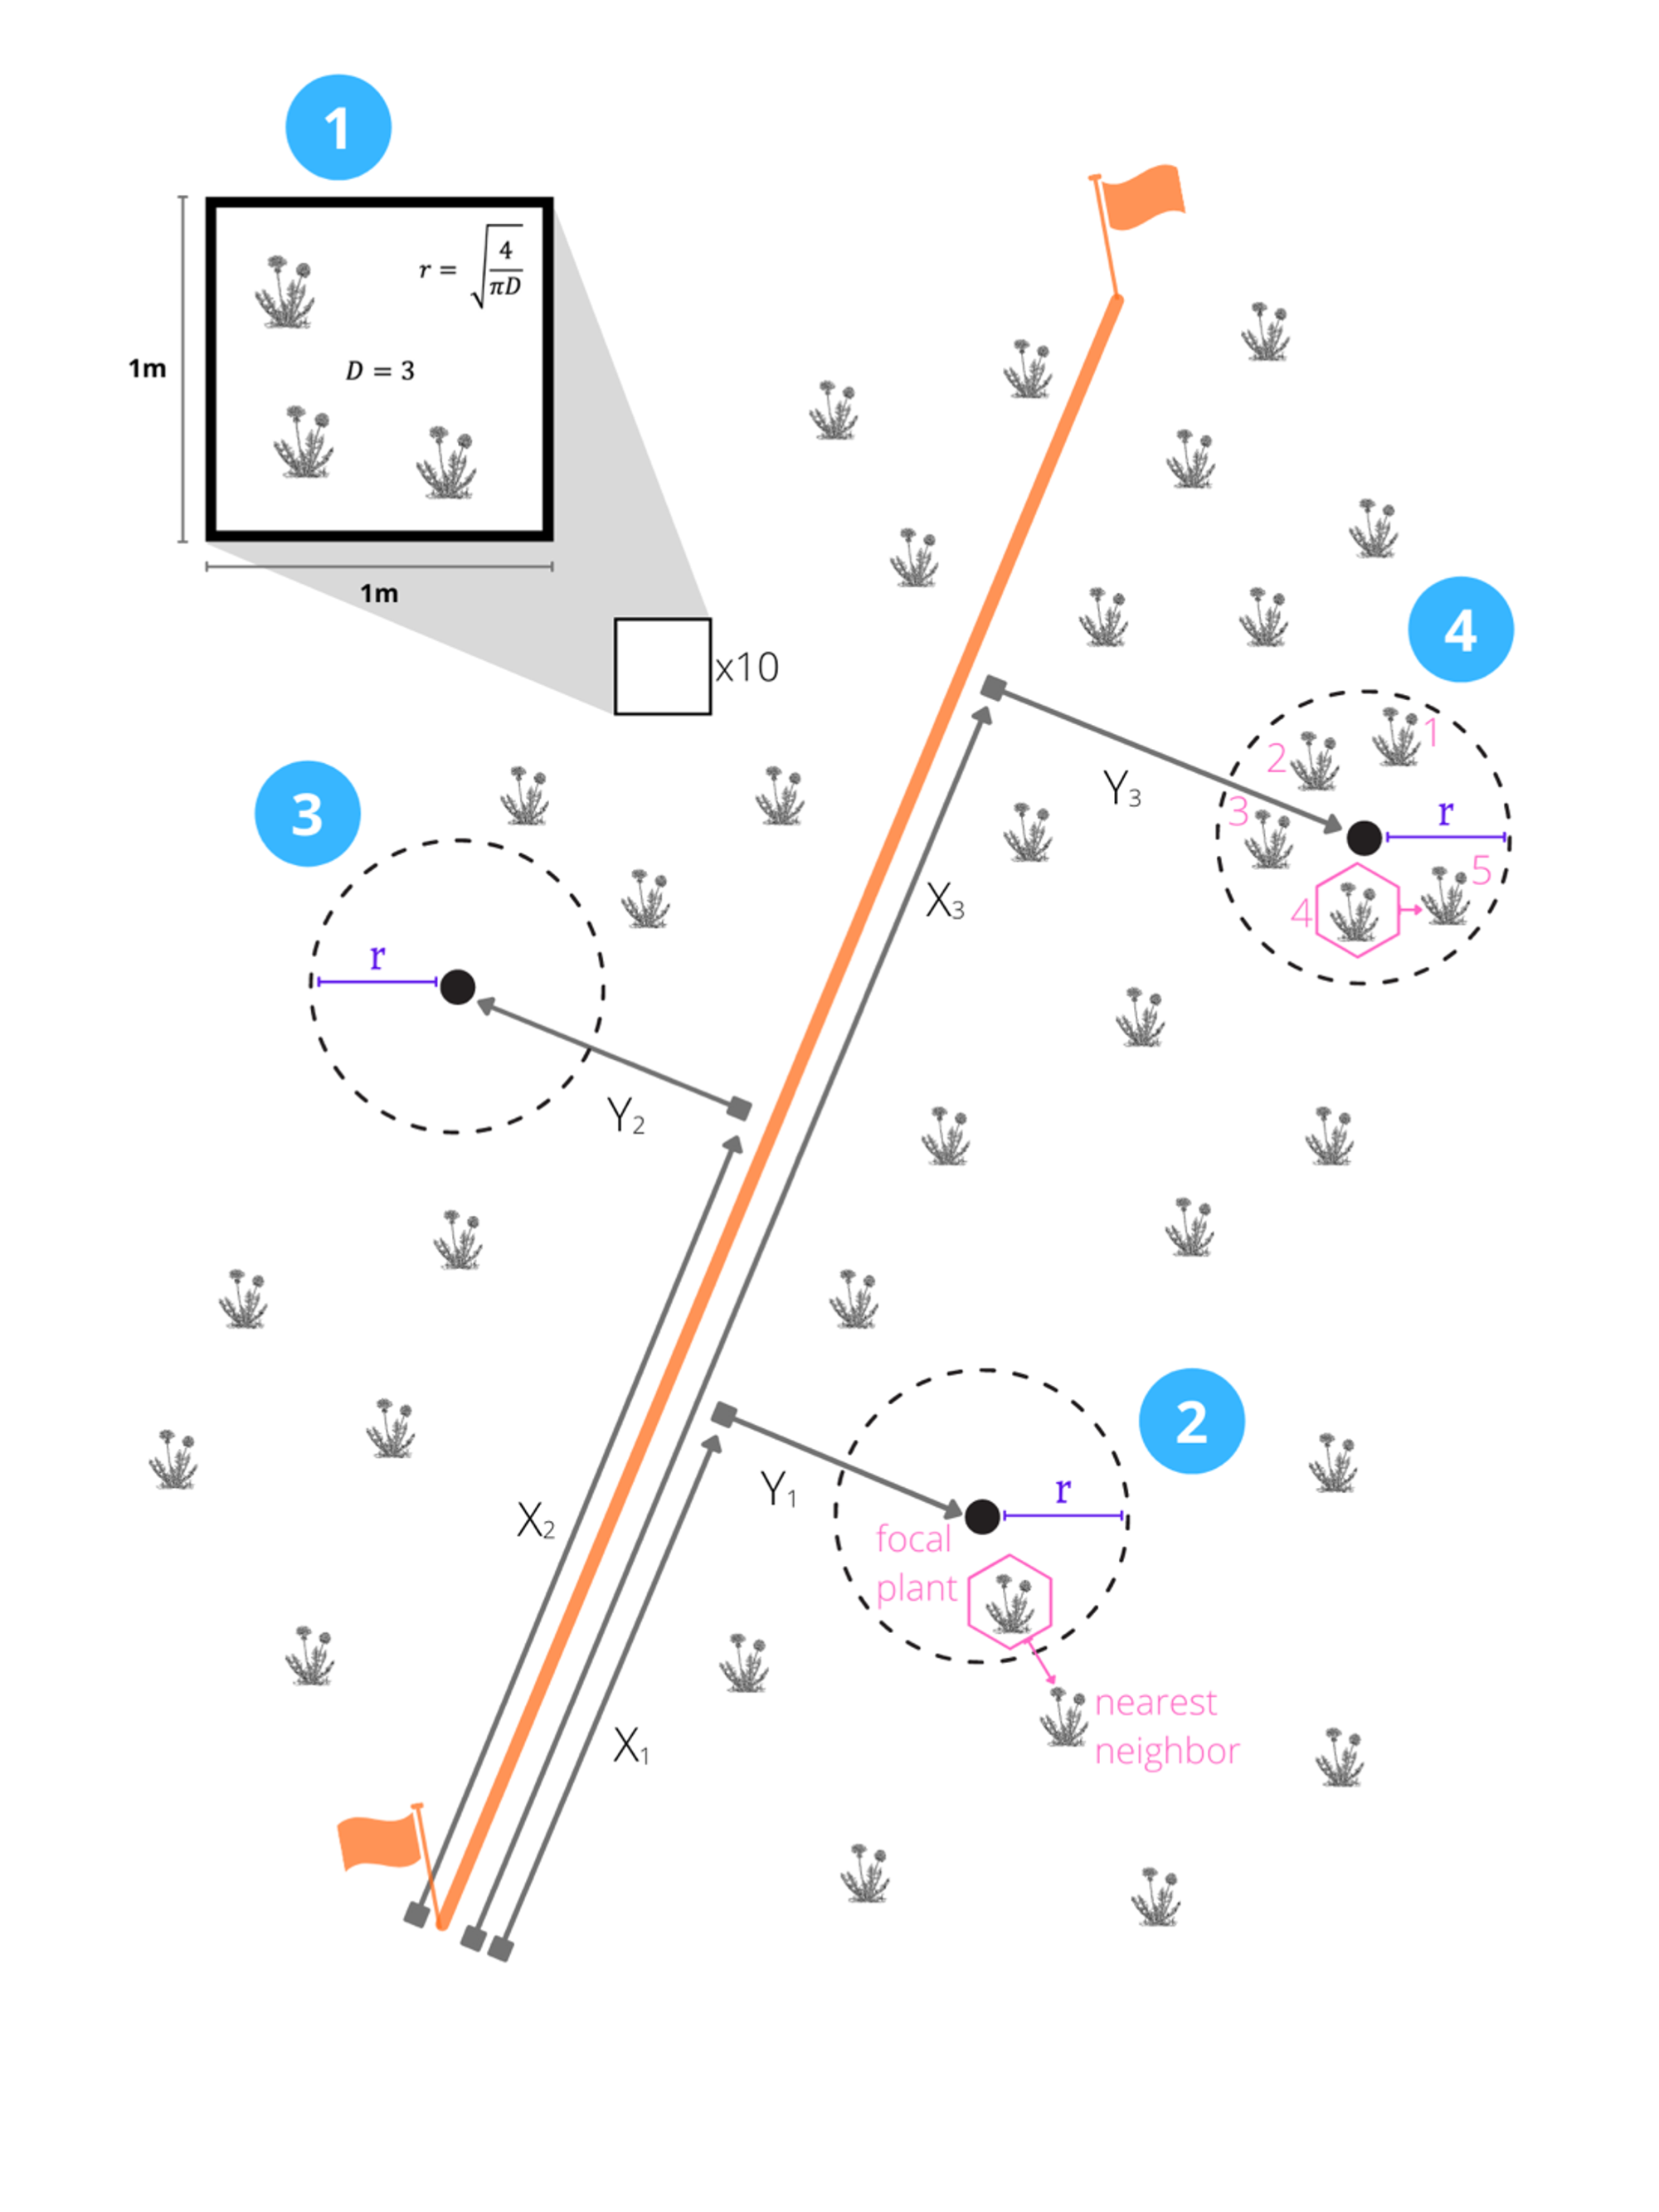
\includegraphics{protocols/images/img1.png}

}

\caption{Fig. 1. A diagram of the sampling scheme described in the text.
(1) Record plant density in 10 randomly located 1-m2 areas to estimate
average plant density D, which is used to calculate quadrat radius r.
(2) A quadrat with one focal plant and its nearest neighbor (outside
quadrat). (3) A quadrat with no focal plants. (4) A quadrat with 5 focal
plants; plant 3 is randomly selected for data collection, and its
nearest neighbor is plant 4. Diagram by Moria Robinson.}

\end{figure}%

\section{Methods Notes}\label{methods-notes}

\begin{enumerate}
\def\labelenumi{\arabic{enumi}.}
\item
  Modifications of this protocol may be necessary to adapt it to
  different systems (see ``Note on Alternate Protocols'' above). If the
  primary protocol won't work for your system, please first consult our
  alternative protocols (see protocol above and ``Protocols - Phase 2''
  folder). If our alternative protocols do not solve the issues, then
  you may adapt the primary protocol as needed. \textbf{Whatever you do,
  please record methods carefully and strive to follow the spirit of the
  protocol and produce comparable data.}
\item
  In Phase 1, collaborators reported that one survey (\textasciitilde60
  plants) took between 0.5 and 2 person days (4-16 hours) using the
  methods above (after a species and site have already been selected).
\item
  We select 40 quadrat center points (instead of 30) so that we have
  extra points ready in case some quadrats are empty. If you predict
  that many quadrats will be empty (e.g., in a very spatially clumped
  population of plants), then select more points (e.g., 60 points).
  (Remember the goal is to have 30 focal plants sampled, plus their
  nearest neighbors).
\item
  Sometimes, especially in small populations, a focal plant ends up
  being another focal plant's neighbor. This is fine. Just note and keep
  going. If you have time, you can add an extra focal plant at the end
  (but this isn't totally necessary).
\item
  For clonal plants, we have been calling stems ``individuals'' if they
  are not connected aboveground. When looking for above ground
  connections, we clear away detritus, but we do not dig or move soil.
  There is also a dedicated alternate protocol for surveying such
  species (see Rhizomatous Geophytes Protocol)
\item
  Please see our Damage Estimation Training Guidelines for guidelines on
  how to estimate herbivore damage. Here are two tips:
\end{enumerate}

\begin{enumerate}
\def\labelenumi{\alph{enumi}.}
\item
  Sometimes discerning herbivore damage from physical damage (e.g.,
  wind, trampling) is tricky. We do the best we can. We look at things
  like how jagged the cut edges are and if they travel past the missing
  area into the remaining leaf tissue (which would suggest the damage
  may have been physical).
\item
  Another challenge is old damage that occurred when leaves were still
  expanding. This could potentially make the area removed seem larger
  than it was. If we suspect something like this happened, then we try
  to bend the leaf back into shape to see if it seems like the missing
  area expanded over time.
\end{enumerate}

\begin{enumerate}
\def\labelenumi{\arabic{enumi}.}
\setcounter{enumi}{6}
\tightlist
\item
  We will accept surveys that only assess damage and do not identify
  herbivores. This will allow people without insect ID skills to
  participate in the study.
\end{enumerate}

\section{Guidelines for Picking Plant
Species}\label{guidelines-for-picking-plant-species-1}

From the patterns found in the first phase of data collection we have
developed the following objectives going forward:

\begin{enumerate}
\def\labelenumi{\arabic{enumi}.}
\item
  Surveys of the three focal species (\emph{Taraxacum officinale},
  \emph{Plantago lanceolata}, and \emph{Plantago major}), especially
  across broad environmental and/or geographic ranges
\item
  Surveys of species in the five focal families (Apocynaceae,
  Asteraceae, Fabaceae, Rubiaceae, and Solanaceae). We want surveys of
  new species within these families, especially species from new clades
  or with unusual growth forms. For repeat surveys of species within
  these families, we are prioritizing surveys from new regions,
  habitats, elevations, etc.
\item
  Surveys of damage to any species' reproductive tissues (e.g., flowers,
  fruits, etc.).
\end{enumerate}

While we welcome all surveys, data that fall under one or more of these
three guidelines is particularly valuable in addressing the current
scope of HerbVar's research questions. Please refer to our more detailed
HerbVar Species Selection Protocol for more information on species
selection and how data contribution relates to authorship in papers
utilizing those data.

\section{Delineating a Site}\label{delineating-a-site}

We realize that defining the `edges' of a site can be subjective and not
easy. We search for an area where a given plant species occurs at a high
enough density to easily select 30 focal plants and 30 unique neighbors
with our method. This is usually a relatively dense patch. Walk around
and see if you see the density drop off to well below the mean density
that is used to calculate radius size. This is usually quite simple,
e.g., when we walk out from the center of a ``site'' and don't see any
individuals of the focal species within 5 m, we decide we're at the edge
of a patch. In some systems, delineating a single, sampleable population
simply might not be possible (e.g., where a species covers a vast area).
In these cases, collaborators should simply do their best to select a
reasonable, representative area to sample.

\section{When to Sample}\label{when-to-sample}

This will depend on the natural history of the system. We will accept
data sampled at any time as long as there has been some herbivory. We
will use the sampling date to examine how herbivory changes seasonally
(please note approximate dates for beginning and end of growing season
for each survey, see siteData sheet in datasheet template). However, the
most valuable surveys will be after enough time has passed for an
ecologically meaningful amount of herbivory to accumulate. In strongly
seasonal systems, this will be in the latter half of the growing season.
But it could also be once leaves have reached maturity (e.g., for
species in which most herbivory is on expanding leaves). In other
systems, the best time to sample might be during or after a key life
history stage (e.g., flowering). All that said, there is no perfect time
to sample. Collaborators should use their knowledge to decide when to
sample (and sample when is feasible; some data is better than no data!).
And repeat sampling is acceptable.

\section{Common Garden Data}\label{common-garden-data}

Common gardens are a powerful tool for studying plant--herbivore
interactions. Several collaborators have proposed including them in
HerbVar, and we would like to try if we can get enough data. To be
applicable to this study a common garden's design would have to be
random with respect to genotype. If a garden was somehow stratified with
blocks containing repeated instances of, e.g., different levels of leaf
toughness, then damage distributions will not be comparable to damage
from wild populations. We may still be able to use such datasets, but
only if we have enough to use them in a separate analysis. Please get in
touch if you would like to contribute common garden data.

\chapter{Damage Estimation}\label{sec-damage}

\section{Overview}\label{overview}

So, you've figured out how to find the random set of plants to score
damage on (e.g., using the Primary Protocol). Now it is time to look
closely at each plant in order to score the amount of damage caused by
herbivores. This is a task that will vary among plant species. This
document is meant to guide you through the process of estimating
herbivore damage using best practices that we have developed. Don't fret
that this document looks too long to follow for 60 plants per survey: we
give an overabundance of pointers to cover likely hiccups that could
occur across the world's 400,000 plant species. Estimating herbivory
will become second nature after you've familiarized yourself with the
methods and had some practice. Ideally with these tips you should be
estimating damage on a single plant in less than five minutes (and maybe
a lot less!).

\textbf{In this document, we provide detail for four key steps from the
Primary Protocol:}

\begin{enumerate}
\def\labelenumi{\arabic{enumi}.}
\tightlist
\item
  Estimating plant size (and determining what tissue counts).
\item
  Counting number of leaves and number of damaged leaves (up to 60 max).
\item
  Estimating percent damage on 10 randomly chosen leaves.
\item
  Estimating percent damage across the whole plant
\end{enumerate}

\begin{tcolorbox}[enhanced jigsaw, opacityback=0, colback=white, breakable, toprule=.15mm, title=\textcolor{quarto-callout-note-color}{\faInfo}\hspace{0.5em}{Note}, left=2mm, coltitle=black, bottomrule=.15mm, arc=.35mm, leftrule=.75mm, rightrule=.15mm, bottomtitle=1mm, toptitle=1mm, colframe=quarto-callout-note-color-frame, colbacktitle=quarto-callout-note-color!10!white, opacitybacktitle=0.6, titlerule=0mm]

If you are just looking for quick tips on estimating percent damage,
skip to \emph{``Estimating Percent Damage on 10 Randomly Chosen
Leaves''} below.

\end{tcolorbox}

\textbf{Two related documents}:

\begin{enumerate}
\def\labelenumi{\arabic{enumi}.}
\item
  The \emph{``Field Guide to Different Types of Herbivore Damage''}
  found in Chapter~\ref{sec-damage}, which has photos of different types
  of damage
\item
  An
  \href{./protocols/Illustrated\%20Guide\%20to\%20Percent\%20Leaf\%20Damage.pdf}{\emph{``Illustrated
  Guide to Percent Leaf Damage''}}, which shows images of leaves with
  different percent damage to help you calibrate your visual estimates.
\end{enumerate}

\textbf{Objectives:} First off, it is good to keep in mind the goals of
these estimates: Ideally, we would like to know (1) the total amount of
plant material consumed by herbivores (e.g., grams of tissue eaten)
\emph{and} the (2) total amount of plant material remaining (e.g., grams
of tissue remaining). Unfortunately, this is not feasible for most
systems, so our goal is to approximate them by estimating (1) plant size
and (2) percent removed by herbivores for entire plants \emph{and} for a
sample of leaves \emph{within} plants.

\begin{tcolorbox}[enhanced jigsaw, opacityback=0, colback=white, breakable, toprule=.15mm, title=\textcolor{quarto-callout-tip-color}{\faLightbulb}\hspace{0.5em}{What kinds of plants will this work for?}, left=2mm, coltitle=black, bottomrule=.15mm, arc=.35mm, leftrule=.75mm, rightrule=.15mm, bottomtitle=1mm, toptitle=1mm, colframe=quarto-callout-tip-color-frame, colbacktitle=quarto-callout-tip-color!10!white, opacitybacktitle=0.6, titlerule=0mm]

This document is written with a focus on vegetative tissue on leafy
plants ≤ 2 m in height. If your plants fit this, then great; read on!

\end{tcolorbox}

\textbf{If your species is a tree or large shrub}, you have two
options:** First, we recommend most HerbVar collaborators restrict
themselves to seedlings and saplings, which we define as ≤ 2 m in
height. In this case, just ignore any individuals \textgreater{} 2 m
tall at your site, and follow the methods below. Make sure to note that
you were excluding mature individuals. If you want to include mature
trees (\textgreater{} 2 m) in your survey, then please follow the
HerbVar Tree Protocol (Chapter~\ref{sec-tree}). The Tree Protocol
describes a method for estimating herbivory on a subsample of leaves on
each tree. However, after you've chosen your subsample of leaves, you
will still have to estimate damage on each leaf, so the damage
estimation tips and illustrated guides below will still be very helpful.

\textbf{If your species is a cactus or other succulent}, then please see
the Cactus and Succulent Protocol (Chapter~\ref{sec-succulents}).

\textbf{If your plants have reproductive tissues} (flowers, fruits,
seeds) and have had them long enough to potentially sustain herbivore
damage, then please see the HerbVar Reproductive Damage Protocol
(Chapter~\ref{sec-repro}) for how to record this damage. The rest of
this document focuses on damage to vegetative tissue.

\section{Estimating Plant Size (and Determining What Tissue
Counts)}\label{estimating-plant-size-and-determining-what-tissue-counts}

In many cases, it will be clear what an individual plant is, but in
cases of clonal plants, we will consider each ramet (i.e., above-ground
unit) to be a unique ``individual.'' Move leaf litter to look for
above-ground connections, but do not clear away soil.

In most cases, herbivores do not eat all plant biomass. Therefore, it
will be useful to note the tissue that you are measuring damage on. For
most HerbVar surveys, this will be vegetative tissue: ``leaves'' and
maybe ``stems.'' The key is to collect your damage estimates across all
of the tissue within a plant or on a random sample of the tissue within
a plant. Before you start estimating damage, give some thought as to
precisely what to include. For example, it is probably best to avoid
senesced leaves (like the brown leaf of the \emph{Lepidium} below)
(perhaps unless the leaves were recently senesced such that they have
not changed in size or distorted in any way). If you need to make any
decisions about what to count, please remember to put detailed notes in
the notes tab of the datasheet.

\begin{figure}

\centering{

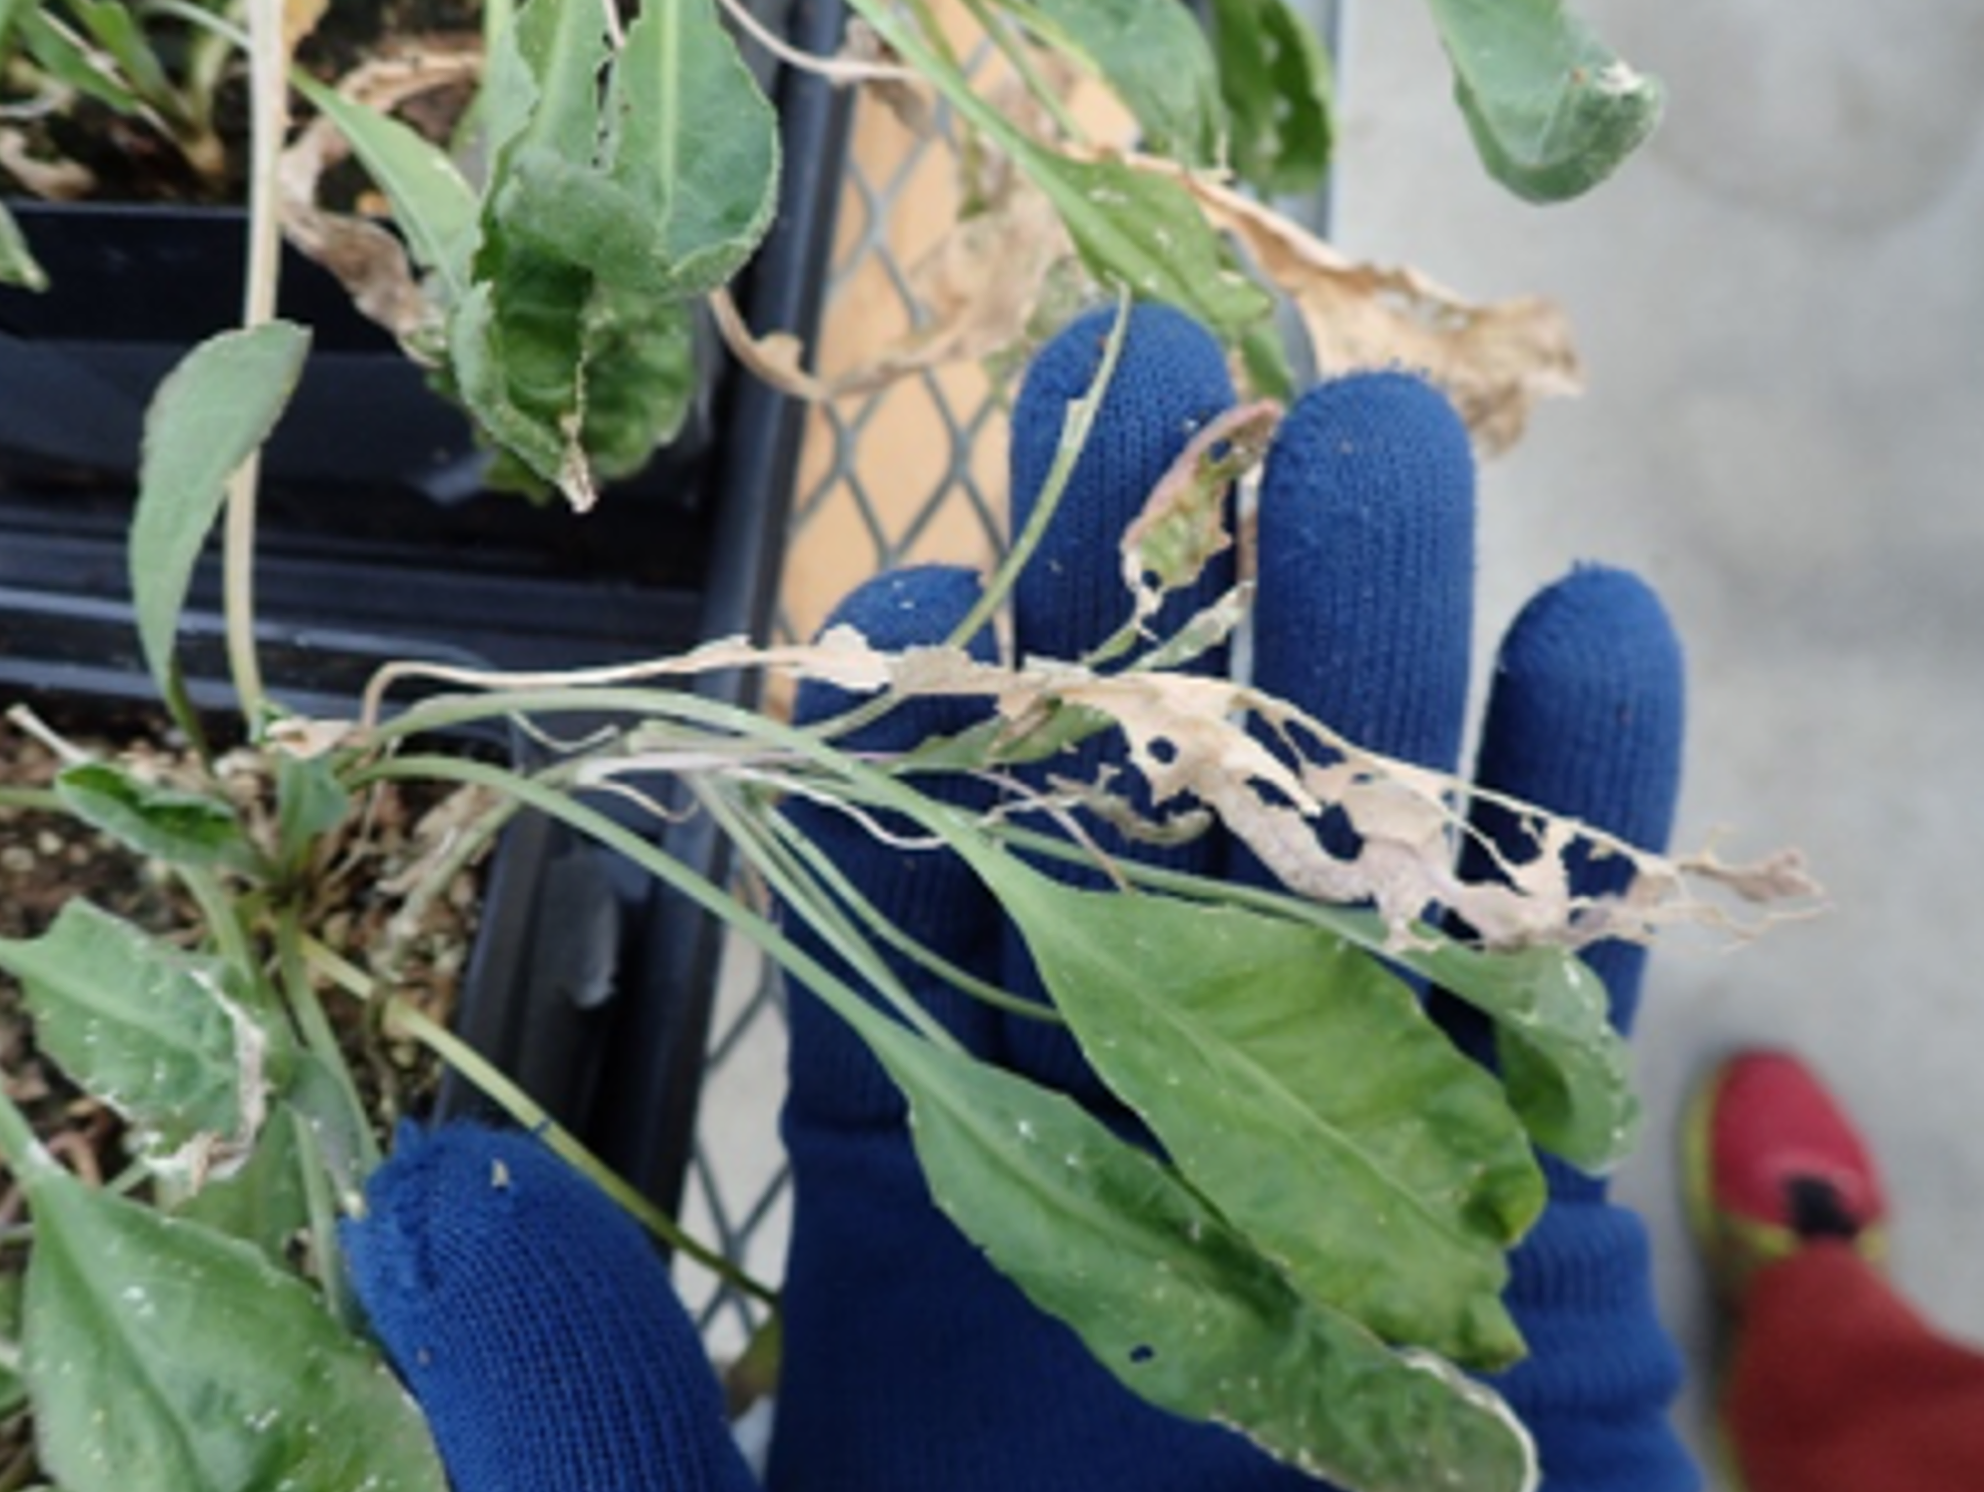
\includegraphics[width=0.8\textwidth,height=\textheight]{protocols/images/img9.png}

}

\caption{\label{fig-lepidium}Lepidium}

\end{figure}%

Once you have decided the extent of plant you will be surveying, you can
measure plant size. Because there are so many different plant growth
forms, we suggest using your judgement to pick the best measure of plant
size for your species. Examples of measures that work well for many
species are standing plant height (e.g., ground to tallest living part),
stem length (better than standing height for creeping species), foliage
diameter, and stem diameter. Just make sure to be consistent within a
survey, and to detail your plant size measure in the notes.

\section{2. Counting Number of Total and Damaged Leaves (up to N =
60)}\label{counting-number-of-total-and-damaged-leaves-up-to-n-60}

The first damage assessment step in the HerbVar Primary Survey Protocol
is estimate the proportion of leaves with any damage, which we are
defining as \textgreater{} 0.5\% of a leaf removed by herbivores. We
estimate the proportion of leaves damaged by counting the number of
undamaged and damaged leaves on each plant (recording total number of
leaves and number of undamaged leaves) up to a max of 60 leaves per
plant. See the following sections and illustrated guides below for tips
on how to decide if a leaf has more than or less than 0.5\% damage. Here
we'll discuss how to choose leaves to examine.

\subsection{Plants with small number of large leaves (N =
1-3)}\label{plants-with-small-number-of-large-leaves-n-1-3}

If you have a plant that has a small number of large leaves (e.g., 1-3),
then the proportion of leaves with damage is not going to be a very
meaningful estimate of overall herbivory. In this case, consider
counting leaflets (instead of leaves), if your plant has leaflets.
Otherwise, proceed with leaves.

\subsection{Plants with \textless60 leaves}\label{plants-with-60-leaves}

If your plant has \textless{} 60 leaves, we encourage you to quickly
count and scan all of the leaves on the plant to look for the presence
of herbivore damage. This will be easy on small plants and harder on
large plants. Either way this step should take less than 2-3 mins. If it
is too time-consuming to look at all the leaves on your plants or even
up to 60 leaves (e.g., leaves are large or complex), then please pick a
feasible number of leaves to subsample, ideally at least up to 30.

\subsection{Plants with \textgreater{} 60
leaves}\label{plants-with-60-leaves-1}

If you are restricted to examining a subsample of leaves within plants
(because your plant have \textgreater{} 60 leaves or because it would be
too time-consuming to do all leaves, then you'll have to decide how to
subsamples leaves within plants. First, you will want to note the size
of the subsample. Ideally you will have one number that will work for
all plants in a survey. In that case, please detail this in the notes.
If you need different subsample sizes for specific plants, please note
subsample size in the notes for each plant, and please also make a note
in the notes tab saying that you had to modify the number of leaves
examined for some plants. Next you'll need a way to subsample leaves
more or less randomly within plants. \textbf{If you need to subsample
within plants, here are four potential methods:}

\subsubsection{Subsampling Method 1:
Nose-Pointing}\label{subsampling-method-1-nose-pointing}

Ian Pearse's nose-pointing method: For large plants, I like to choose
four positions around the plant roughly at the cardinal directions (this
never comes out as neatly as I might like since a lot of plants just
don't grow that way). I stand at each of those positions, I turn away
from the plant, I close my eyes, and I put my finger against my nose,
like this (below). Then, I turn facing the plant, open one eye, and I
choose whatever leaf I am pointing to (or the closest leaf if I'm
pointing to multiple or none). I've done this on a lot for leaves, and I
think it would basically work for other tissues (twigs, flowers, etc).
You can continue to do this until you have examined your full subsample
of leaves. Caveats: It is important to include mostly-eaten leaves using
this method, but the method probably underestimates damage because you
are less likely to be randomly pointing at a mostly-eaten leaf-nub.

\begin{figure}

\begin{minipage}{0.50\linewidth}

\centering{

\includegraphics{protocols/images/img10.png}

}

\subcaption{\label{fig-nose}Is that creep trying to pick his nose with
his thumb? No.~This is the nose pointing method to acquire a random
sample of plant parts. The creep/researcher establishes a fixed point in
his field of vision with an ``L''-shaped hand position while turned away
from the plant.}

\end{minipage}%
%
\begin{minipage}{0.50\linewidth}

\centering{

\includegraphics{protocols/images/img11.png}

}

\subcaption{\label{fig-point}He then turns to the plant, opens a single
eye, and chooses the leaf that he is pointing to.}

\end{minipage}%

\end{figure}%

\subsubsection{Subsampling Method 2: True
Randomization}\label{subsampling-method-2-true-randomization}

True randomization: Assign all leaves, seeds, etc. on the plant a random
number, draw N numbers, and measure damage on those leaves. Caveats:
this is rigorous, but probably too time consuming for most plants (and
you'd probably just as well measure the damage on all the leaves you've
given a number to!).

\subsubsection{Subsampling Method 3: Arbitrary
Sampling}\label{subsampling-method-3-arbitrary-sampling}

Arbitrary sampling. That sneaker-word, arbitrary! This is basically to
say ``I really tried to choose an unbiased sample of the plant tissue,
but I have no idea whether or not I succeeded.'' Caveats: Clearly, this
can have problems, but it's what we're probably left with in most cases
where plants have complicated architecture, the tissue is hard to choose
in a more truly randomized way, or you're just strapped for time.

\subsubsection{Subsampling Method 4: Define Your Own
Method}\label{subsampling-method-4-define-your-own-method}

Design (and make notes of!) your own subsampling scheme. Can you choose
every seventh (or random-numberedth leaf along a shoot of skunkbush
sumac (right)? Note how you did it, and approximately how much of the
plant tissue you sampled (e.g., \% of poison ivy sampled).

\begin{figure}

\centering{

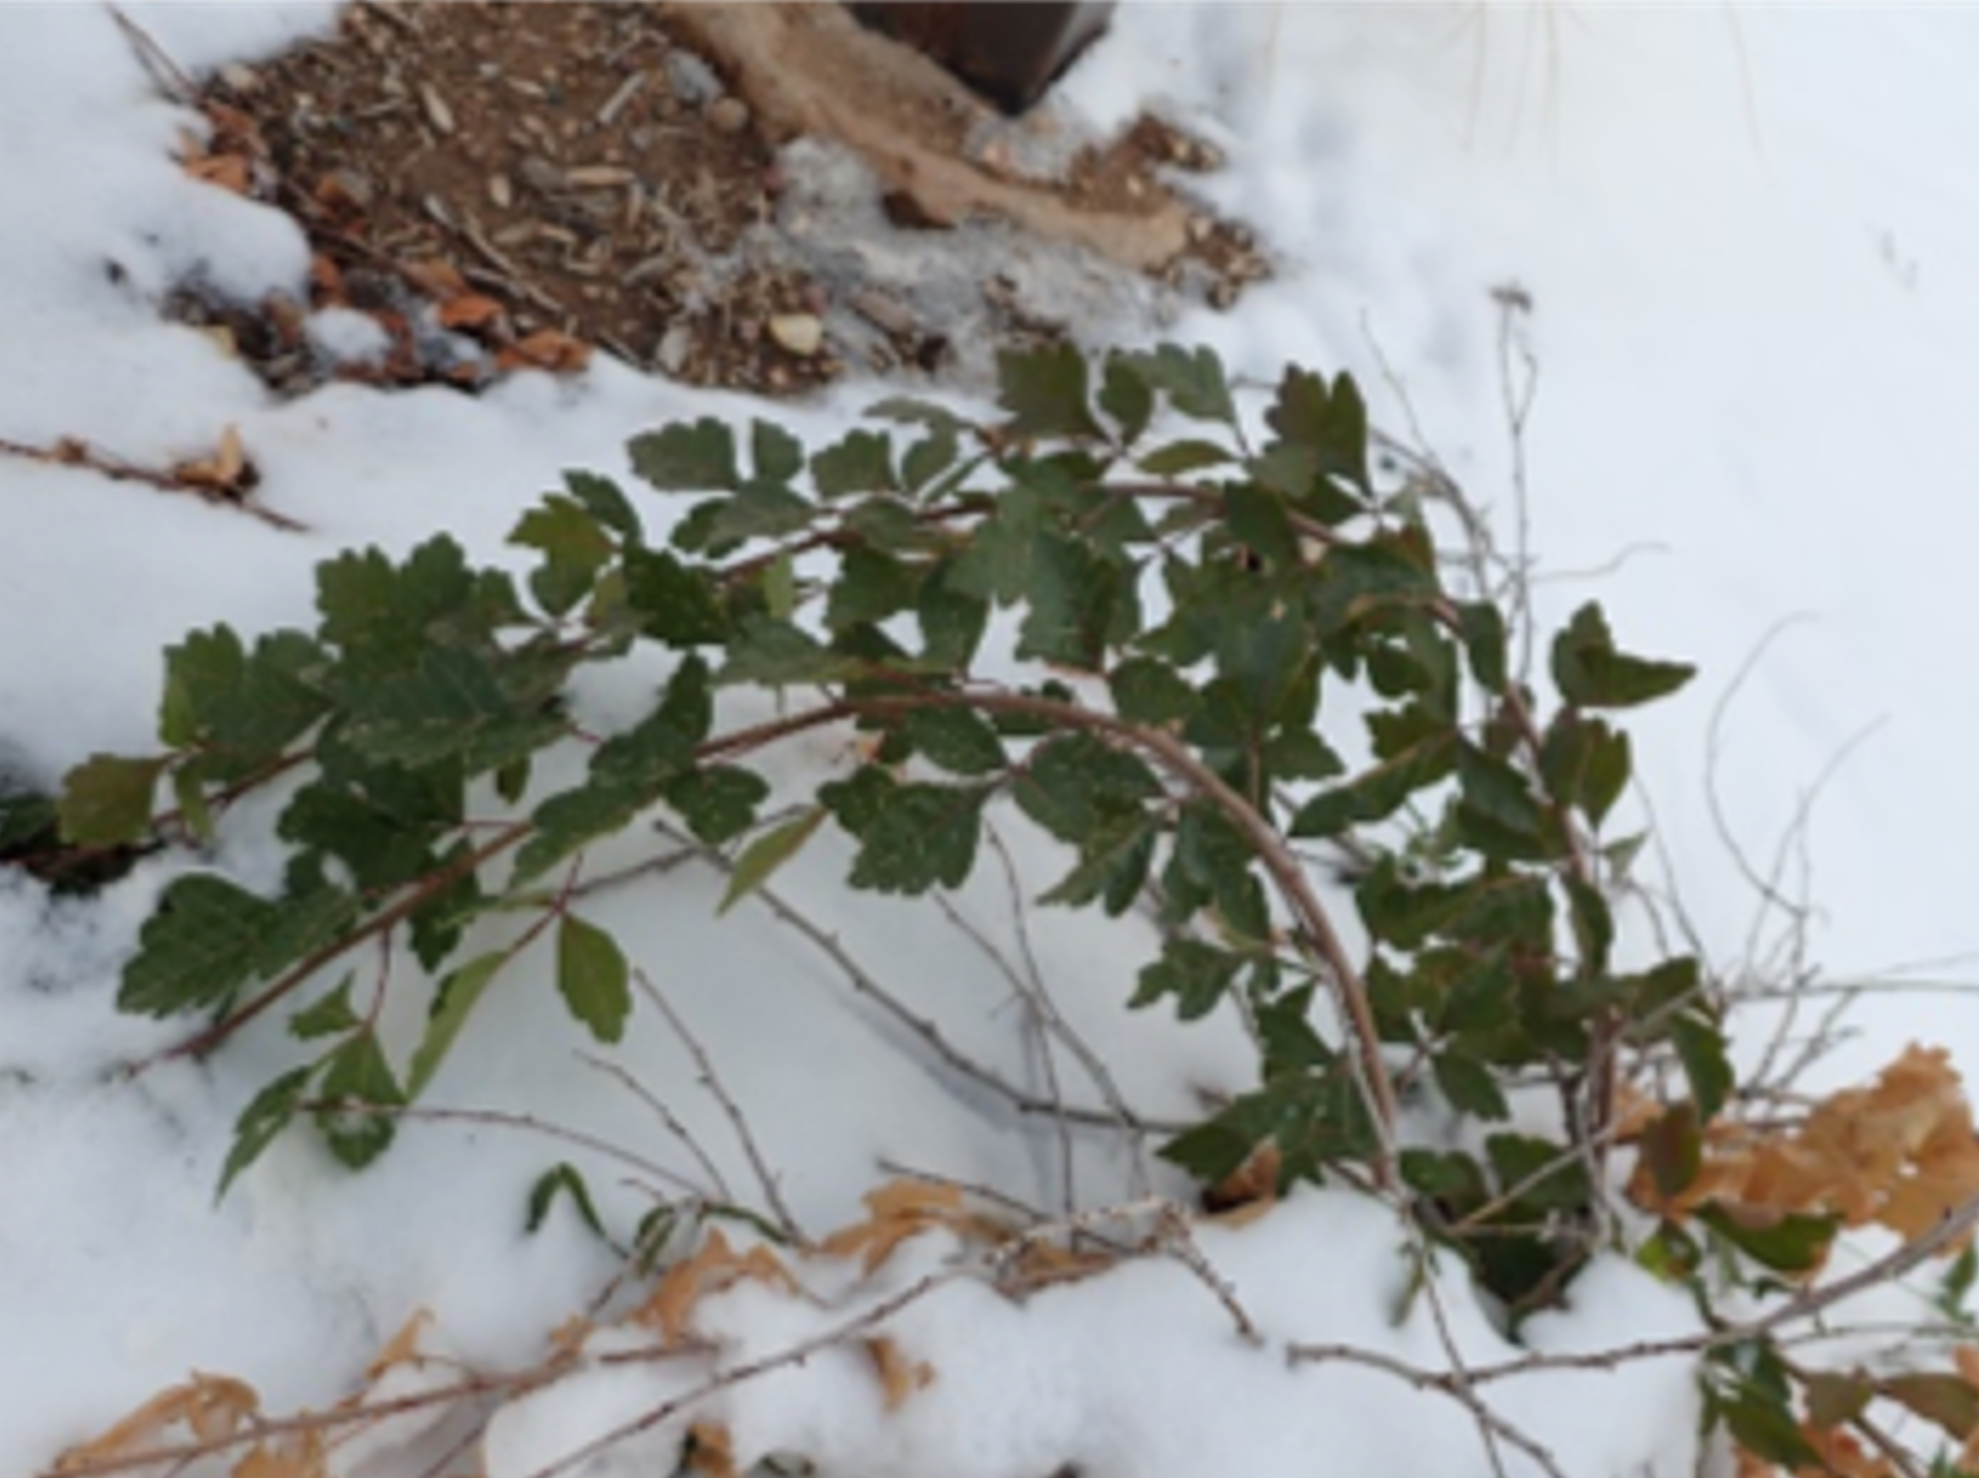
\includegraphics[width=0.7\textwidth,height=\textheight]{protocols/images/img12.png}

}

\caption{\label{fig-random}legend needed}

\end{figure}%

\begin{tcolorbox}[enhanced jigsaw, opacityback=0, colback=white, breakable, toprule=.15mm, title=\textcolor{quarto-callout-tip-color}{\faLightbulb}\hspace{0.5em}{Philosophical thoughts about counting damaged leaves}, left=2mm, coltitle=black, bottomrule=.15mm, arc=.35mm, leftrule=.75mm, rightrule=.15mm, bottomtitle=1mm, toptitle=1mm, colframe=quarto-callout-tip-color-frame, colbacktitle=quarto-callout-tip-color!10!white, opacitybacktitle=0.6, titlerule=0mm]

This method works well (we think) as an estimate of overall herbivory
for plants with small leaves or leaflets (e.g., sagebrush,
\emph{Astragalus}, locust), but will be very imprecise for plants with
fewer, larger leaves because most large leaves will have some damage,
though maybe not much. So, this is probably ineffective for your
Welwitschia or banana tree. However, because counting a few large leaves
is easy, we suggest doing it anyway for completeness.

\begin{figure}[H]

\centering{

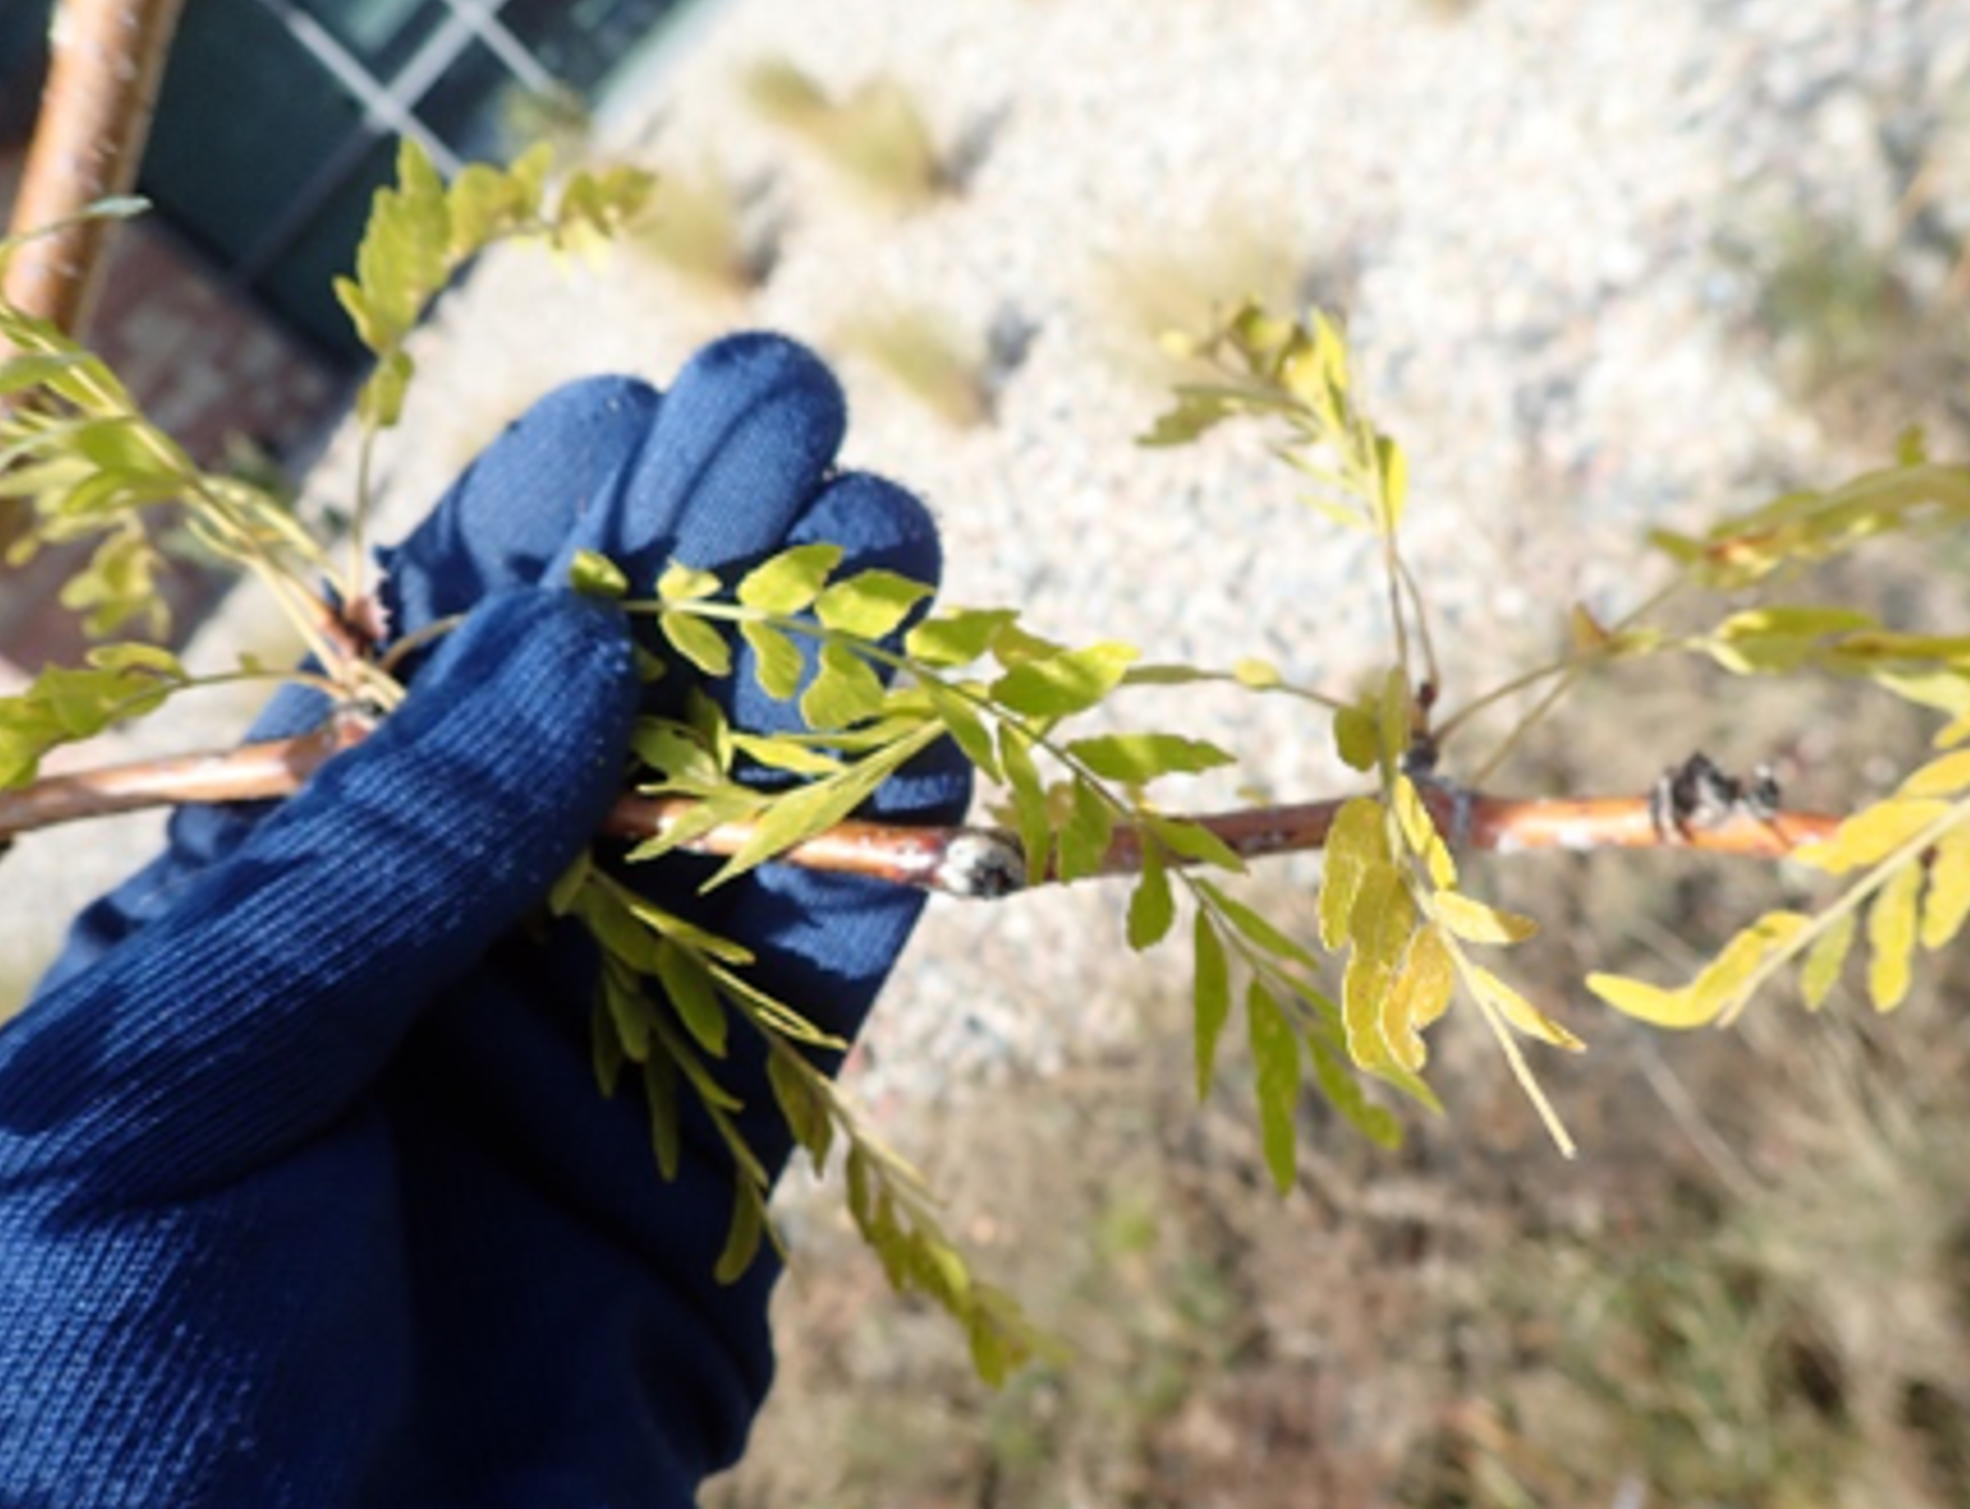
\includegraphics[width=0.7\textwidth,height=\textheight]{protocols/images/img13.png}

}

\caption{\label{fig-arbitrary}legend needed}

\end{figure}%

\end{tcolorbox}

\section{3. Estimating Percent Damage on 10 Randomly Chosen
Leaves}\label{estimating-percent-damage-on-10-randomly-chosen-leaves}

The next damage assessment step is estimating percent damage on 10
randomly chosen leaves. Well actually, the 10 data columns for this step
(percLf1--percLf10) come after the column for whole plant percent damage
(percHerbPlant) in the HerbVar template datasheet, but it makes more
sense, in this document, to discuss percent herbivory on individual
leaves before discussing whole plant percent herbivory.

\subsection{Randomly choose 10 leaves:}\label{randomly-choose-10-leaves}

If your plant has 10 or fewer leaves, then please examine them all; if
your plant has more than 10 leaves, then use one of the methods above to
choose 10 leaves randomly. Strive to have these leaves be an unbiased
subsample of all the leaves on the plant.

\subsection{Estimate percent damage on each
leaf}\label{estimate-percent-damage-on-each-leaf}

Finally, the main event---this is probably the main reason you're
reading this document. There are many ways to estimate percent damage on
leaves. For HerbVar, we recommend collaborators use visual estimation
because other methods are slower and would make the sample sizes we need
to describe herbivory distributions unattainable. Moreover, careful
visual estimation does a surprisingly good job, especially after some
practice, especially if the primary goal is to compare the frequency of
plants with low and high herbivory, as ours is. However, we strongly
recommend checking your estimates against estimates from other observers
using the same method, or even better against estimates using digital
methods (i.e., LeafByte) to get a sense for how good of a job you are
doing, and if you are overestimating or underestimating.

\subsubsection{Visual estimation}\label{visual-estimation}

Visual estimation is essentially as simple as it sounds. You look at a
leaf and eyeball what percent was removed or damaged by herbivores. The
benefit of this method is that it is quick, allowing us to obtain the
large sample sizes we need to describe whole herbivory distributions.
The caveat is that this method has more measurement error than other
methods. For example, Zoe and Julie and Marc Johnson have found that
visual estimation tends to overestimate damage by a few percent,
particularly for researchers with less experience. We hope to mitigate
estimation error with the guidelines below, our Illustrated guide to
amounts of percent damage, an online training quiz, and a
ground-truthing effort. First we explain how to estimate damage. Second,
we explain how to make sure you're doing a good job.

\begin{enumerate}
\def\labelenumi{\arabic{enumi}.}
\tightlist
\item
  How to estimate damage
\end{enumerate}

Record estimates at a high resolution. We usually record at a resolution
of 2.5\% (Table 1). This may seem like unreasonably high resolution when
you first try, but with a little practice and calibration you will get
surprisingly good. We encourage trying for high resolution
because---even with considerable error---high resolution estimates will
likely be closer to the true values on average than estimates reported
as broad categories (e.g., 0\%, 1-10\%, 11-25\%, 26-50\%\ldots{} too
coarse!). Plus, if you report your best guesses we can model the error
statistically; we're out of luck if you just report broad categories.

Table 1. Recommended resolution for recording percent herbivory

Percent Meaning 0\% No herbivory 0.5\% A trace amount of herbivory 1\%
\textasciitilde1\% herbivory 2.5\% \textasciitilde2.5\% herbivory 5\%
\textasciitilde5\% herbivory 7.5\% \textasciitilde7.5\% herbivory So
forth Up to 100\% (e.g., everything removed except base of leaf petiole)

\begin{enumerate}
\def\labelenumi{\arabic{enumi}.}
\setcounter{enumi}{1}
\item
  When you first look at a leaf, do a quick mental calibration before
  estimating damage. We do this by visualizing cutting the leaf into a
  range of proportions. Start with large proportions and scale down to
  your finest resolution (e.g., 2.5\%). For example, think about what
  half the leaf would look like, then imagine a quarter (25\%) of the
  leaf. Do the same for a tenth of the leaf (10\%): imagine 10
  equally-sized divisions in the leaf. How big is each tenth? Then
  mentally cut each tenth in half to get 20 divisions of 5\% leaf area.
  Finally, half of each of those units would be 2.5\% leaf area. How big
  is that?
\item
  When it is time to do the actual herbivory estimate, one strategy that
  works well for contiguous blocks of damage is to use fractional
  thinking to zero in on the precise value, starting with larger
  fractions and gradually working your way down to smaller
  fractions---honing from a coarse estimate to a precise estimate. For
  example,

  \begin{itemize}
  \item
    If \textasciitilde12.5\% of a leaf were damaged, then\ldots{}

    \begin{itemize}
    \tightlist
    \item
      Mentally cut the leaf into quarters
    \item
      See that less than a quarter (25\%) is damaged
    \item
      Mentally cut the quarter with damage in half, yielding eighths
      (12.5\%)
    \item
      See that the area damaged is equal to an eighth and record 12.5\%
    \end{itemize}
  \item
    If \textasciitilde30\% of a leaf were missing, then\ldots{}

    \begin{itemize}
    \tightlist
    \item
      Mentaly cut the leaf in half
    \item
      See that less than half is damaged
    \item
      Mentally cut the leaf into quarters
    \item
      See that more than a quarter (25\%) is damaged
    \item
      Take mental note of the 25\% damaged, and then focus on estimating
      how much more than that 25\% is damaged
    \item
      Mentally halve the quarter of the leaf with the excess damage
      above 25\%, yielding eighths (12.5\%)
    \item
      See that the damage above 25\% is a little less than half of one
      of those eighths, which means it's a little less than a sixteenth
      or 6.25\%
    \item
      25\% plus a little less than 6.25\% comes close to 30\%, record
      it!
    \end{itemize}
  \end{itemize}
\item
  If your leaf has more than one area of damage, try mentally
  consolidating each area of damage into one area and then estimate the
  size of that using the method above. Alternatively, if mental
  consolidation isn't working well, you can mentally divide the leaf
  into fractions that are as small as the smallest patch of herbivore
  damage. Then simply mentally tally the number of patches of that size
  that would be damaged.
\item
  An acetate grid can be a very helpful tool. Some people use them to
  help guide their estimates on every leaf. Others use them occasionally
  for validating and calibrating estimates (e.g., on the first few
  leaves estimated each day). To make one, simply print out a grid cell
  on a transparency (make sure it's printer-friendly). Ian tends to
  print out several grid-sizes, and uses the size that has at least 20
  grid cells for most leaves. Put the grid against the leaf. Count the
  number of grid cells with leaf (or where leaf should be) = T. Count
  the number of grid cells with damage = D. Percent damage is 100*D/T.
  If you have 40 grid cells per leaf, then each grid cell will be 2.5\%,
  a good target resolution. If you only have 20 grid cells per leaf, you
  can count in units of half grid cells to obtain a finer resolution.
  Ian likes the grid method, as he can do it while on a ladder. It has
  the downsides of being hard on oddly-shaped leaves (where most grid
  cell readings are exterior), only estimating damage with a resolution
  of 1/T, and probably overestimating some damage types (like some
  beetle feeding) that may damage small parts of each grid cell.
\item
  For complexly pinnate leaves (e.g., Apiaceae), it is probably best to
  divide the leaf into leaflets or pairs of leaflets, then follow the
  methods above.
\item
  If damage is very high and very little leaf tissue remains, take a
  large and small leaf and compare the leaf base width, petiole and
  midrib size to compare. Use these comparisons to visually reconstruct
  the leaf, and deduce \% damage from there
\item
  If you have marginal damage on leaves with non-smooth margins: If you
  draw an entire margin a third of the way between the base of the
  margin teeth and tip of the margin teeth, this approximately results
  in the same area measurement as if you had actually drawn in the
  margins---but it is easier/more accurate to imagine/draw a straight
  line than margin teeth
\item
  Piercing-sucking damage, when visible, should be mentally consolidated
  and estimated similarly to chewing damage. Be careful about confusing
  piercing-sucking damage and disease because they often look similar.
  If you are unsure, sleuth around your site to see if you can find the
  culprit in action. Sometimes it helps to find leaves that have damage
  at different stages of progression. This will let you reconstruct what
  older more necrotic tissue (and less discernible) might have looked
  like before it became so necrotic, perhaps inferring the cause of the
  damage. If this doesn't help, consult someone who may be able to or
  pick another species to survey.
\end{enumerate}

\begin{figure}

\centering{

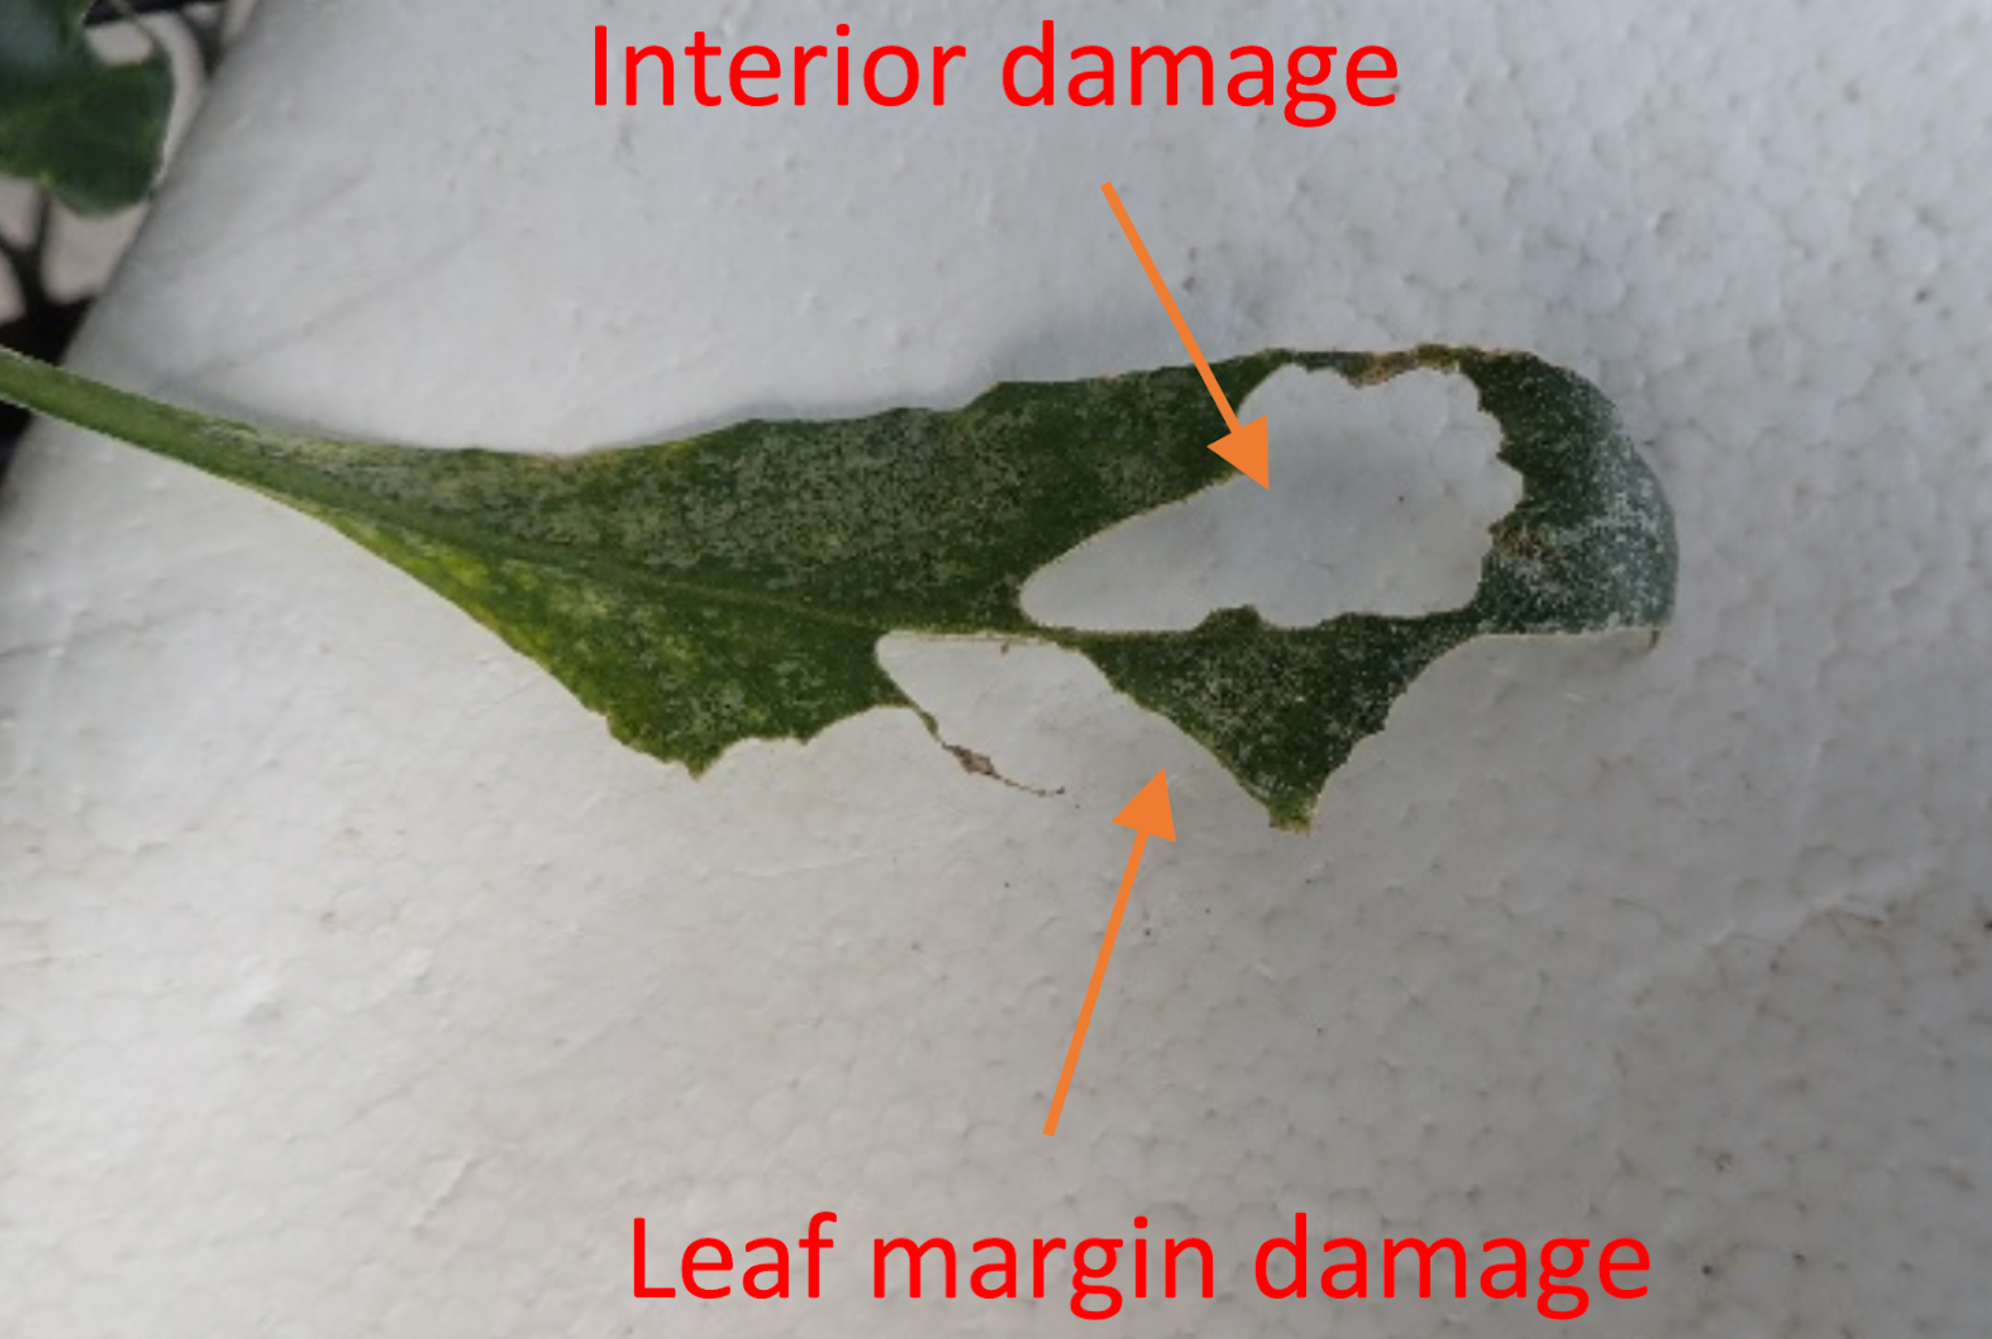
\includegraphics{protocols/images/img14.png}

}

\caption{\label{fig-location}Legend Needed.}

\end{figure}%

\begin{enumerate}
\def\labelenumi{\arabic{enumi}.}
\setcounter{enumi}{9}
\item
  For leaves with herbivore-built leaf shelters (rolls and ties), please
  carefully peer into or open shelters to estimate damaged area and
  count resident herbivores.
\item
  Through all of this, make sure you are correctly identifying what is
  herbivore damage versus disease versus physical damage. Please have a
  look at our A field guide to types of plant damage. We are trying to
  avoid damage caused by pathogens or abiotic stress. Before each
  survey, spend some time studying the range of damage types on plants
  in your population. Try to get a sense for what types of damage you
  might see during the survey. Sleuth out what damage types might just
  be physical damage (e.g., from wind). In this sleuthing, we have found
  it helpful to search for clues at both broad and fine scales. At broad
  scales, we search many plants across each site to see if we can find
  what is causing a particular type of damage. Often we will find the
  culprit, but only after a broad search. At fine scales, we use a hand
  lens to look closely at the damage. Often, a closer look at the
  damaged edges of a leaf reveals marks from insect mandibles. Tearing,
  in contrast, tends to be cleaner and more angular, often following
  even small leaf veins. Wind damage can manifest as browning. Look to
  at damaged spots to see if any tissue is actually missing. Only
  include necrotic tissue as herbivory if you are certain it is from
  herbivory. If you cannot be confident in your ability to tell apart
  physical and herbivore damage for a particular species or site, then
  please do not do the survey or consult someone who can help you.
\item
  For internal feeding insects (e.g., hackberry psyllids, below):

  \begin{itemize}
  \item
    Count discrete units: count either the number of insects or the
    number of galls or mines. There are columns in the Template
    Datasheet for galls and mines.
  \item
    Mines should be included in percent damage and counted as discrete
    units.
  \item
    Galls should only be counted, not included in percent damage because
    galls are actually extra tissue! The removed tissue is internal and
    can't be seen.
  \item
    Keep an eye out for signs of stem-boring insects. Sometimes these
    can be counted.
  \end{itemize}
\end{enumerate}

\begin{figure}

\centering{

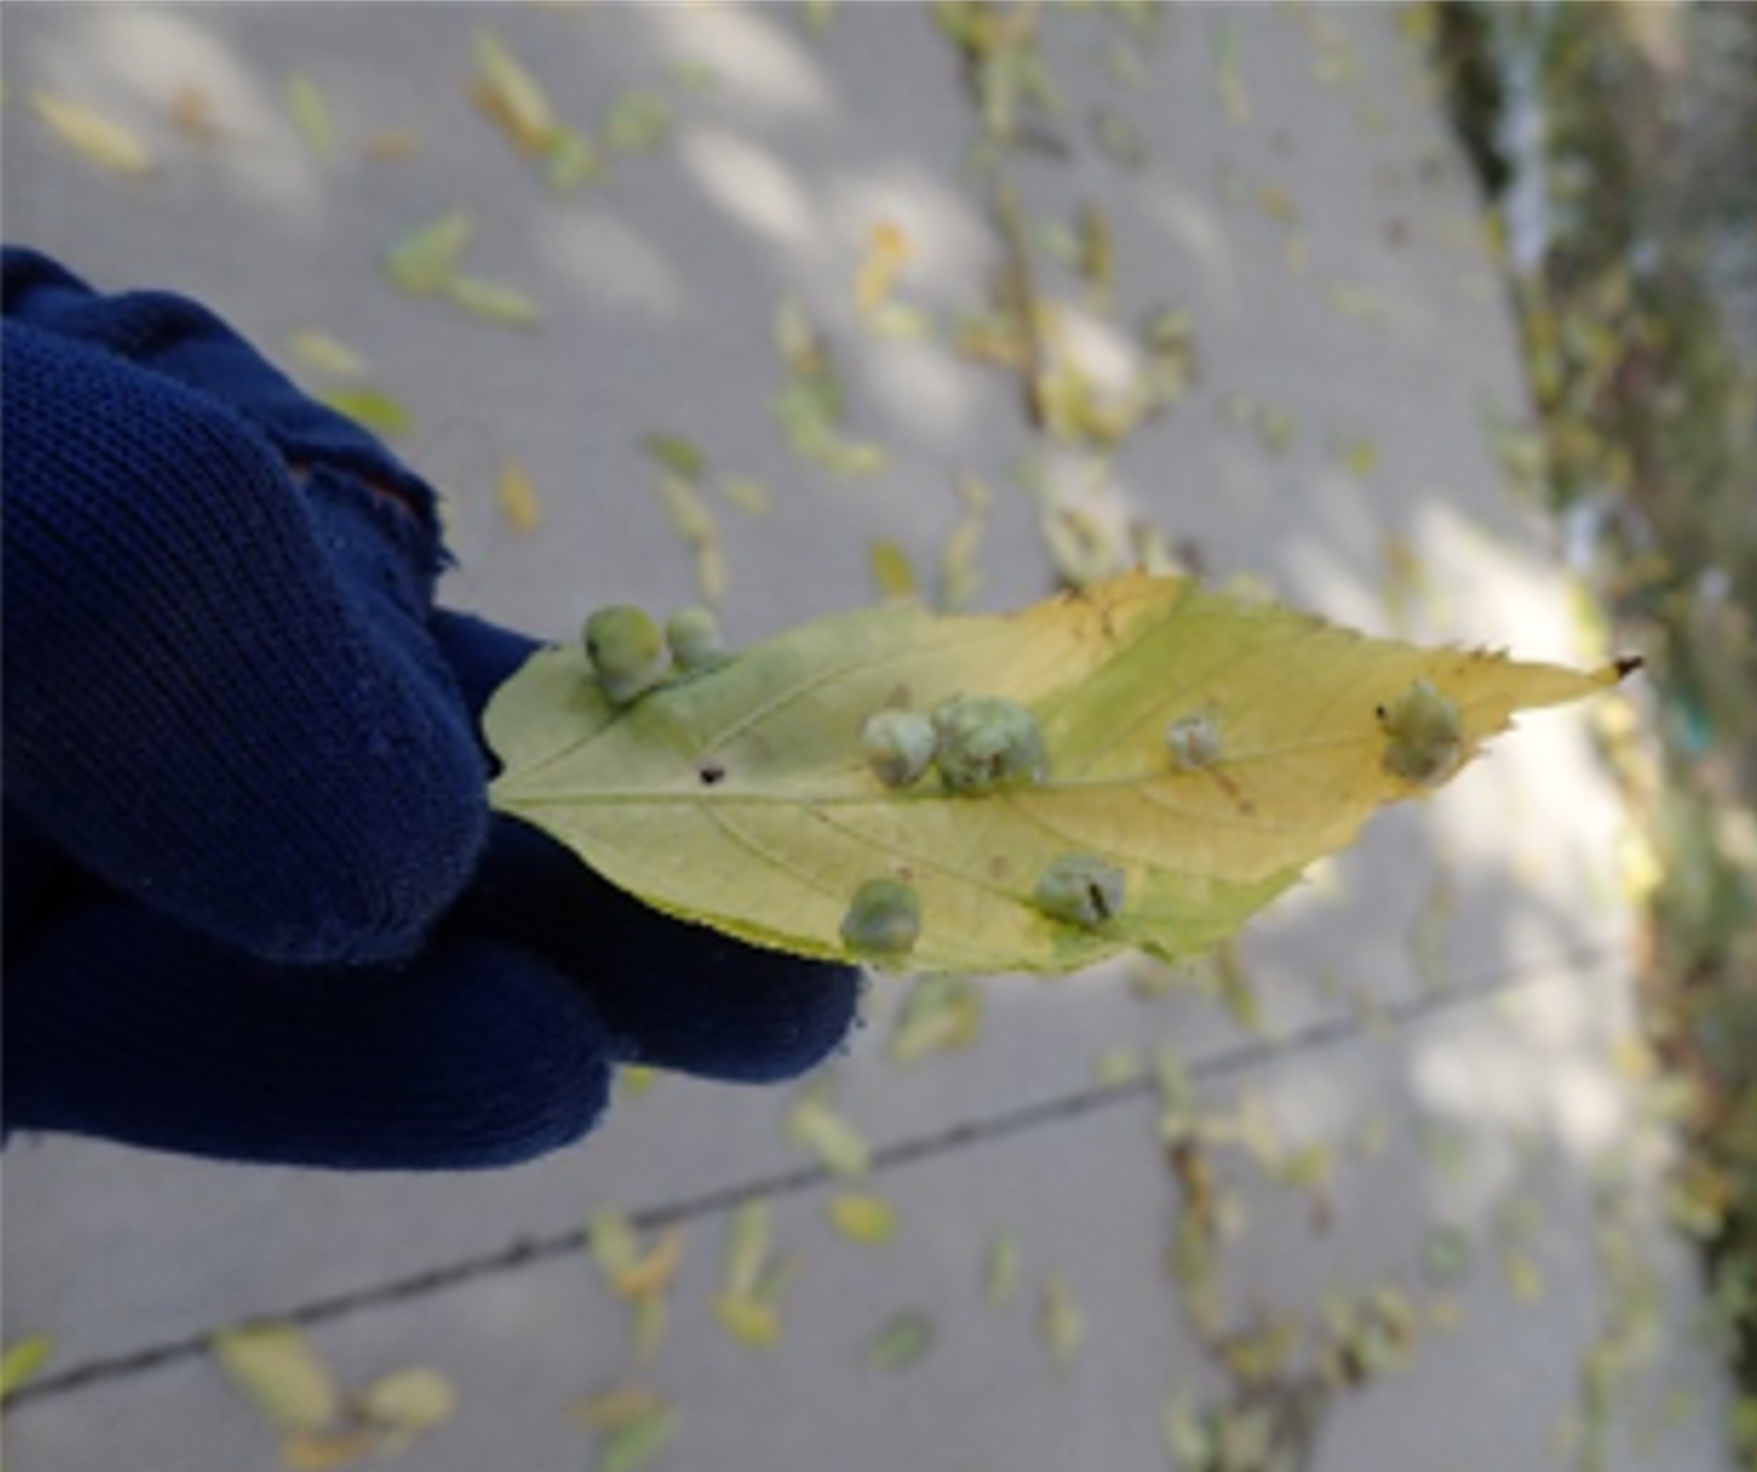
\includegraphics{protocols/images/img15.png}

}

\caption{\label{fig-internal}Internal feeding insects}

\end{figure}%

\subsubsection{How to make sure you're doing a good
job}\label{how-to-make-sure-youre-doing-a-good-job}

\begin{enumerate}
\def\labelenumi{\arabic{enumi}.}
\item
  Be conscious that most people overestimate low levels of tissue damage
  (Johnson 2016). Try to correct for this by being aware of this
  tendency, not rounding up at low levels of damage, and
  calibrating/validating estimates on leaves with low damage.
\item
  Invest time in practicing, calibrating, and validating estimates.
  Especially do this before collecting data, and continue to calibrate
  and validate regularly through data collection.
\item
  Standardize among observers you work with or have a single observer
  for all estimates.
\item
  Print out An illustrated guide to amounts of percent damage. Study it
  while practicing, and take it into the field with you as a reference.
  You can focus on the pages with leaves that are most similar in shape
  to leaves from your species.
\item
  Take our online herbivory estimation training quiz (in development, we
  will add the link here when it's ready). This will help you assess
  your accuracy and precision and give you additional practice in
  estimating herbivory. We suggest re-taking this quiz once per week
  when doing surveys to refresh your memory.
\item
  Finally, ground truth a subset of your damage estimates using a
  digital method. When doing this, please use 6 randomly selected plants
  in each survey. Do the survey as normal, but after visually estimating
  herbivory on each leaf in those plants use one of the two digital
  methods below to get a digital herbivory estimate (LeafByte or
  ImageJ). Make sure to record a unique identifier for each leaf to link
  visual and digital estimates.

  \begin{itemize}
  \item
    LeafByte: This is an app developed recently by scientists at Cornell
    (including our very own Zoe Getman-Pickering and Julie Davis). It
    goes on your iPhone and estimates damage of leaves that you
    photograph (it will tell you total leaf area, total damage area, and
    proportional damage). You can download the app and read instructions
    here. `BioLeaf' is a similar app for Android phones.
  \item
    Scan leaves and estimate damage with Image J. For this, I usually
    collect leaves into a little bag. Once I'm back in the lab, I tape
    the leaves to a sheet of paper, and then use Image J (free software
    here) to estimate leaf damage. This is similar to LeafByte, but it
    takes longer.
  \end{itemize}
\end{enumerate}

\begin{figure}

\centering{

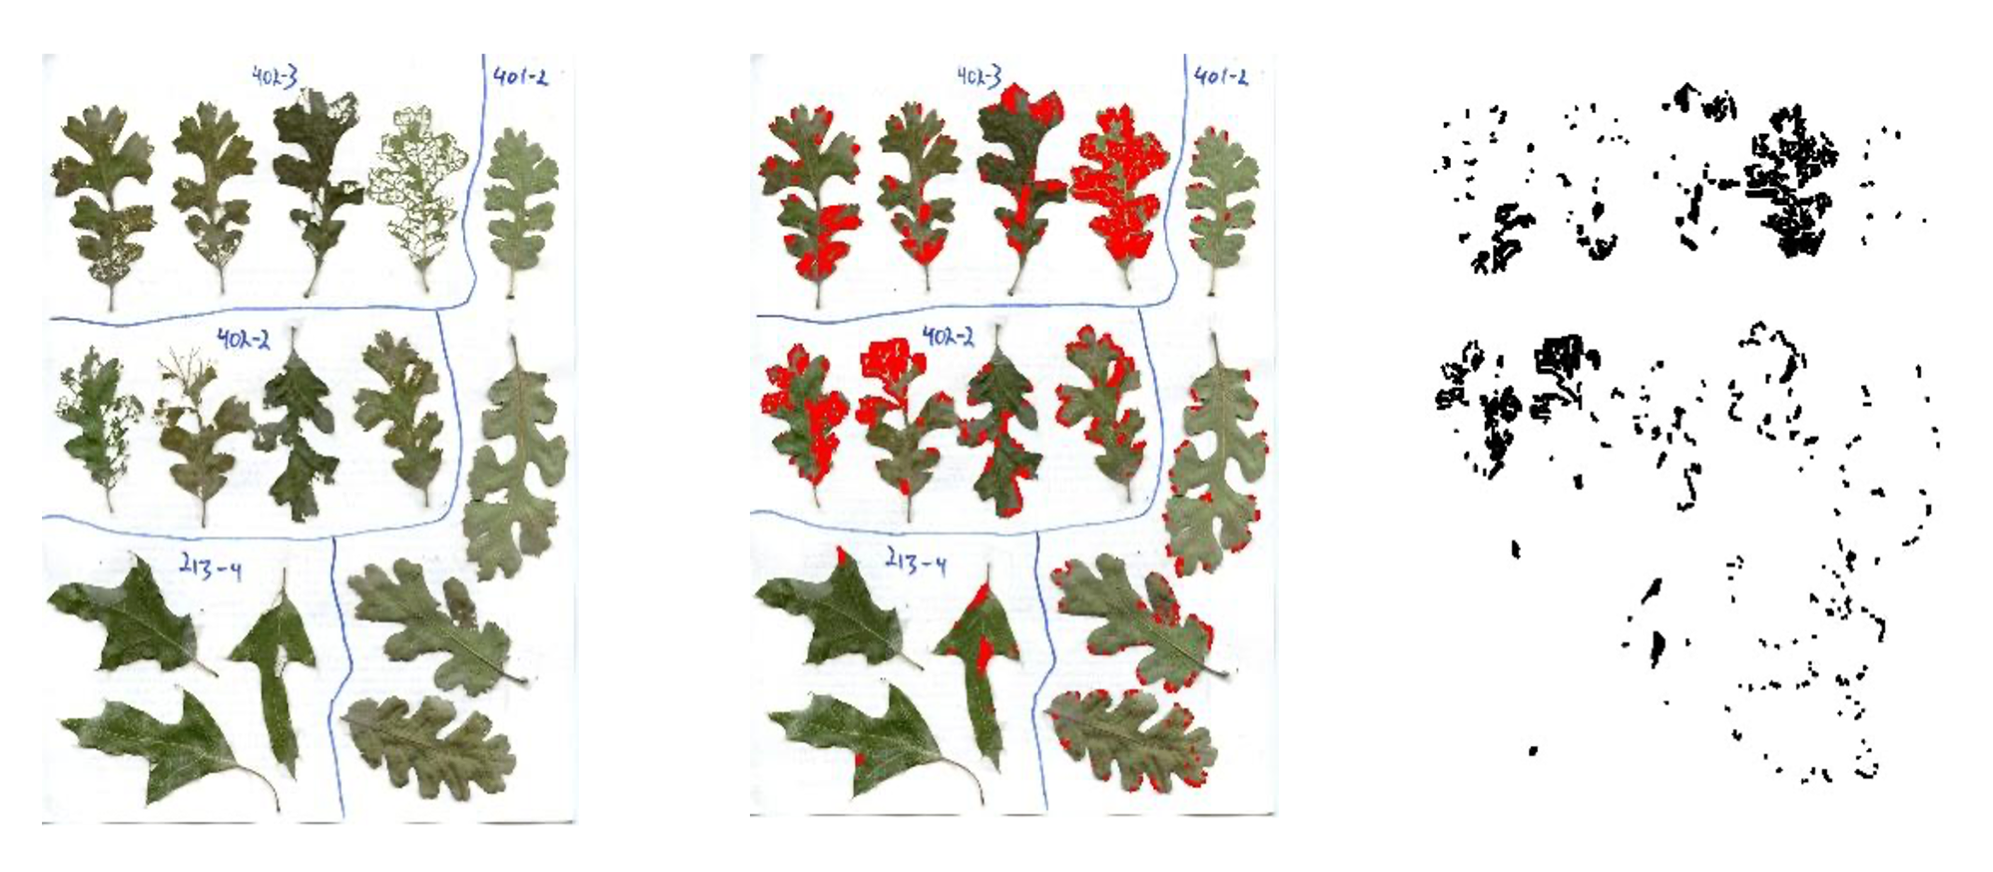
\includegraphics{protocols/images/img16.png}

}

\caption{\label{fig-imagej}Three steps in measuring damage with Image
J.}

\end{figure}%

\section{4. Estimating Percent Damage Across the Whole
Plant}\label{estimating-percent-damage-across-the-whole-plant}

The final damage assessment step is estimating percent damage across the
whole plant, or as much of the plant as is feasible. We encourage you to
strive to look across entire plants when estimating whole plant
herbivory (unless your plants are \textgreater{} 2 m in height, in which
case please follow the HerbVar Tree Protocol). For larger plants, there
will be significant estimation error, but it is probably less than the
error associated with subsampling, which could miss hotspots of
herbivory within plants. Remember, the goal is just a visual estimate.
You'd be surprised how quickly you can scan and integrate across a whole
plant to estimate herbivory. However, we acknowledge this may not be
feasible for large or complex plants; in those cases, please use one of
the subsampling methods above and remember to record your methods and
the size of your subsample. If you don't feel that a whole-plant
estimate is feasible, record the percent damage on 30 random leaves (see
\#3 above) and carefully record the total number of leaves on the plant
and number of damaged leaves on the plant. The whole plant herbivory can
be calculated from these values post hoc.

\subsection{Tips for visually estimating damage across the whole
plant:}\label{tips-for-visually-estimating-damage-across-the-whole-plant}

Effective methods will vary a lot based on the size of plants, size of
leaves, and architecture of plant. For smaller plants with a smaller
number of leaves, you can quickly estimate damage on each leaf and
combine leaf-level estimates into a plant-level estimate. If all leaves
are similar in size, you can just average them. If leaves vary in size,
you will need to take their relative sizes into account.

We often find it helpful to pick a reference leaf size on which to base
mental calculations. Often it's convenient to pick the largest or
smallest leaf, depending on whether you prefer scaling down or scaling
up leaf level estimates.

An important tip to remember for speed is that when plants have more
than \textasciitilde9 leaves, leaves with low levels of damage will
contribute very little to plant-level damage. For example, a leaf with
2\% damage would only contribute 0.2\% to overall plant damage on a
plant with 10 similarly sized leaves. This means that you do not need to
stress about these leaves. Of course, if every leaf on the plant has 2\%
damage, then this would be important to keep track off. Indeed, this is
essentially what you need to pay attention to as you scan the whole
plant. In our experience, most plants have skewed distributions of
herbivory within plants, so it's all about paying attention to the
proportion of leaves with insignificant and significant herbivory and
the amount of herbivory on leaves with significant herbivory. But this
isn't always the case, so look out for more even within-plant
distributions. (Side note: we hope to get at this question with our
herbivory estimates on the 10 random leaves). For larger plants and
plants with many small leaves, it is impractical to scan each individual
leaf and mentally combine them (unless you are a mental math wizard!).
In these cases, we still encourage you to scan the whole plant, but
simply increase the grain size of your focus. For example, estimate
herbivory at the scale of similarly sized branches of leaves. For plants
with many, many small leaves, you may need to squint and look at
similarly sized clumps of leaves. For example, people who work on
conifers have a method for estimating herbivory on branches that
involves looking up through a branch and seeing how much sky shows
through.

Please let us know if you have additional tips, suggestions, or
guidelines we can add to this document. And please let us know if
anything is missing, confusing, or wrong! Have fun in the field and be
safe.

\begin{tcolorbox}[enhanced jigsaw, opacityback=0, colback=white, breakable, toprule=.15mm, title=\textcolor{quarto-callout-important-color}{\faExclamation}\hspace{0.5em}{Important}, left=2mm, coltitle=black, bottomrule=.15mm, arc=.35mm, leftrule=.75mm, rightrule=.15mm, bottomtitle=1mm, toptitle=1mm, colframe=quarto-callout-important-color-frame, colbacktitle=quarto-callout-important-color!10!white, opacitybacktitle=0.6, titlerule=0mm]

If you're in an area with tick-borne diseases, don't forget to check for
ticks after!

\end{tcolorbox}

\chapter{Reproductive Damage}\label{sec-repro}

This protocol aims to assess damage by insect herbivores to reproductive
parts of plants (i.e., flowers, fruits, and/or seeds). This is a
supplement to the Primary Protocol, which aims to randomly select and
sample 30 plants, plus their nearest conspecific neighbor, within a
population.

\textbf{Objectives: }The goal is to measure the proportional damage to
reproductive organs on each plant within the surveyed population. That
is, for each individual plant we will record the number of damaged and
undamaged reproductive organs. Ideally, these measurements should be
taken as supplemental data for the same individual plants (focal and
neighbor plants) for which leaf damage was taken for the primary
protocol, although reproductive damage measurements are welcome from
other plant populations from which no leaf damage measurements have been
taken.

\section{Protocol}\label{protocol}

\begin{enumerate}
\def\labelenumi{\arabic{enumi}.}
\tightlist
\item
  \textbf{Select a species to survey}: We are hoping to get broad
  taxonomic and geographic coverage of damage to reproductive organs.
  Therefore, any species could be surveyed. However, to ensure that the
  data are comparable across sites/species/families/etc, the plants
  should have the following characteristics:
\end{enumerate}

A. At least half of the individuals at your site should possess
reproductive material. If most of the plants are in a vegetative stage,
you probably won't be able to survey enough reproductive individuals to
get a decent sample size. Ideally, \textgreater30 of the sampled plants
will have reproductive damage data

B. Each individual plant should produce enough flowers/fruits/seeds so
that you can survey between 15-30 reproductive units per plant. These
`units' could be flowers, fruits, or seeds, whichever will give you
enough things to count.

\begin{enumerate}
\def\labelenumi{\roman{enumi}.}
\item
  E.g., if your plants have just a few fruits, try opening fruits and
  counting a random sample of seeds, which could get you higher numbers.
  If some plants have fewer units (\textasciitilde5-10
  flowers/fruits/pods/seeds), that is okay, as long as most have at
  least 15.
\item
  If your species typically has only one or a few flowers, we have
  provided a modified protocol below
\end{enumerate}

C. Most of the plants should be in a similar phenological stage. If
there is a mixture of flowering and fruiting plants within the
population, it might be difficult to get a large enough sample size for
one organ type. Additionally, different phenological stages will likely
be attacked by different insects

D. If your plant does not meet these requirements, please skip measuring
damage to reproductive organs. That's okay. Or get in touch if you have
questions

\begin{enumerate}
\def\labelenumi{\arabic{enumi}.}
\setcounter{enumi}{1}
\item
  Use the Primary Protocol to establish a transect, pick/calculate a
  quadrat radius, and randomly select focal/nearest neighbor plants
\item
  Identify the reproductive tissue you will be surveying, e.g., flowers,
  fruits, pods, seeds, etc.
\item
  For each plant then record (see Fig 1):
\end{enumerate}

A. Phenology of the plant (i.e., budding, flowering, fruiting, etc.)

B. Total number of units examined

C. Herbivore damage per unit: Either percent or count of injuries

D. Pathogen damage per unit

E. Unknown damage per unit (i.e., any damage not attributable to either
herbivores or pathogens)

F. Ideally at least 30 reproductive units will be examined per plant.
For plants that have much more than 30 units, examine a haphazard
subsample of 30 units per plant. These should be sampled from different
parts of the plant to obtain a good representative sample of damage
levels to the plant. Damage measurements will be highly variable among
species, depending on the types of flowers or fruits produced as well as
the type of damage that is most common in the population. Below we give
some general guidelines.

G. There likely will need to be modifications for some species, but we
trust collaborators to do the best they can in their systems while
maintaining the overall spirit of the protocol. For example, if your
species has only one or a few flowers/fruit, you can estimate the damage
as a percentage. Keep in mind that the goal is to capture the
variability in damage rates among plants within a population, so you
will want to choose a measure of flower/fruit/seed damage that best
captures this variability.

\subsection{Data Recording Tips}\label{data-recording-tips}

\textbf{Record the following data in the provided printable and digital
datasheets.}

\begin{enumerate}
\def\labelenumi{\arabic{enumi}.}
\item
  Start by surveying the type of damage that is most common on the
  reproductive structures of plants in the population. Look for damage
  by insects that may chew on developing flowers (e.g.~katydids,
  beetles), insects that bore into flower heads or seeds (e.g.~larval
  weevils, leps, or flies), or true bugs that may probe/pierce into the
  seeds or fruits (looks like little black dots on the fruits). In many
  cases you will need to tear open the seed head/fruit to look for
  boring insects inside the seeds/fruit.
\item
  Look for signs of chewing damage inside the fruit, such as destroyed
  seeds and insect frass.
\item
  The best measurements of damage will depend on the type and extent of
  damage present. If the plant species experiences damage to multiple
  organs (e.g., petals, stamens, etc.), focus on the damage to the
  primary reproductive parts if it is not feasible to measure multiple
  organs.
\item
  In the ``reproUnit'' column of the reproData sheet in the template
  Excel datasheet, please record what organs you are recording damage on
  (e.g., stamens, petals for flowers). If present and identifiable,
  record the number and identity of the florivore, frugivore, seed
  predator
\item
  If your species has only one or a few flowers per plant and it's
  possible to record the percent damage to a flower or fruit, you can
  record these percent damages in the percR\# columns. 15 such columns
  are provided but please add more if you are able to record the
  per-unit damage of more than 15 reproductive structures
\item
  Indicate whether you are recording `count' or `percent' damage in the
  `damageUnit' column.
\end{enumerate}

\begin{figure}

\centering{

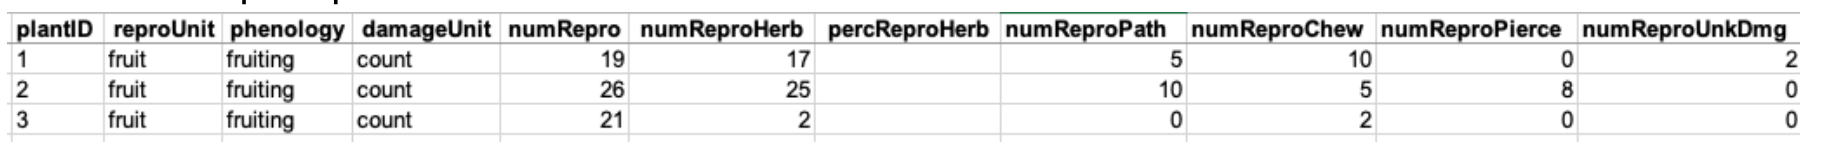
\includegraphics{protocols/images/img28.png}

}

\caption{\label{fig-reprotable}Example reproData information}

\end{figure}%

Note 1: numReproHerb can be less than the sum of the counts of types of
damage because a single reproductive unit can have multiple types of
damage.

Note 2: In the damageUnit column, record `count' or `percent' depending
on whether you are recording the number of damage reproductive units or
the percent damage to a single unit

\subsection{Examples of different types of damage to reproductive
material}\label{examples-of-different-types-of-damage-to-reproductive-material}

\begin{figure}

\begin{minipage}{0.50\linewidth}

\centering{

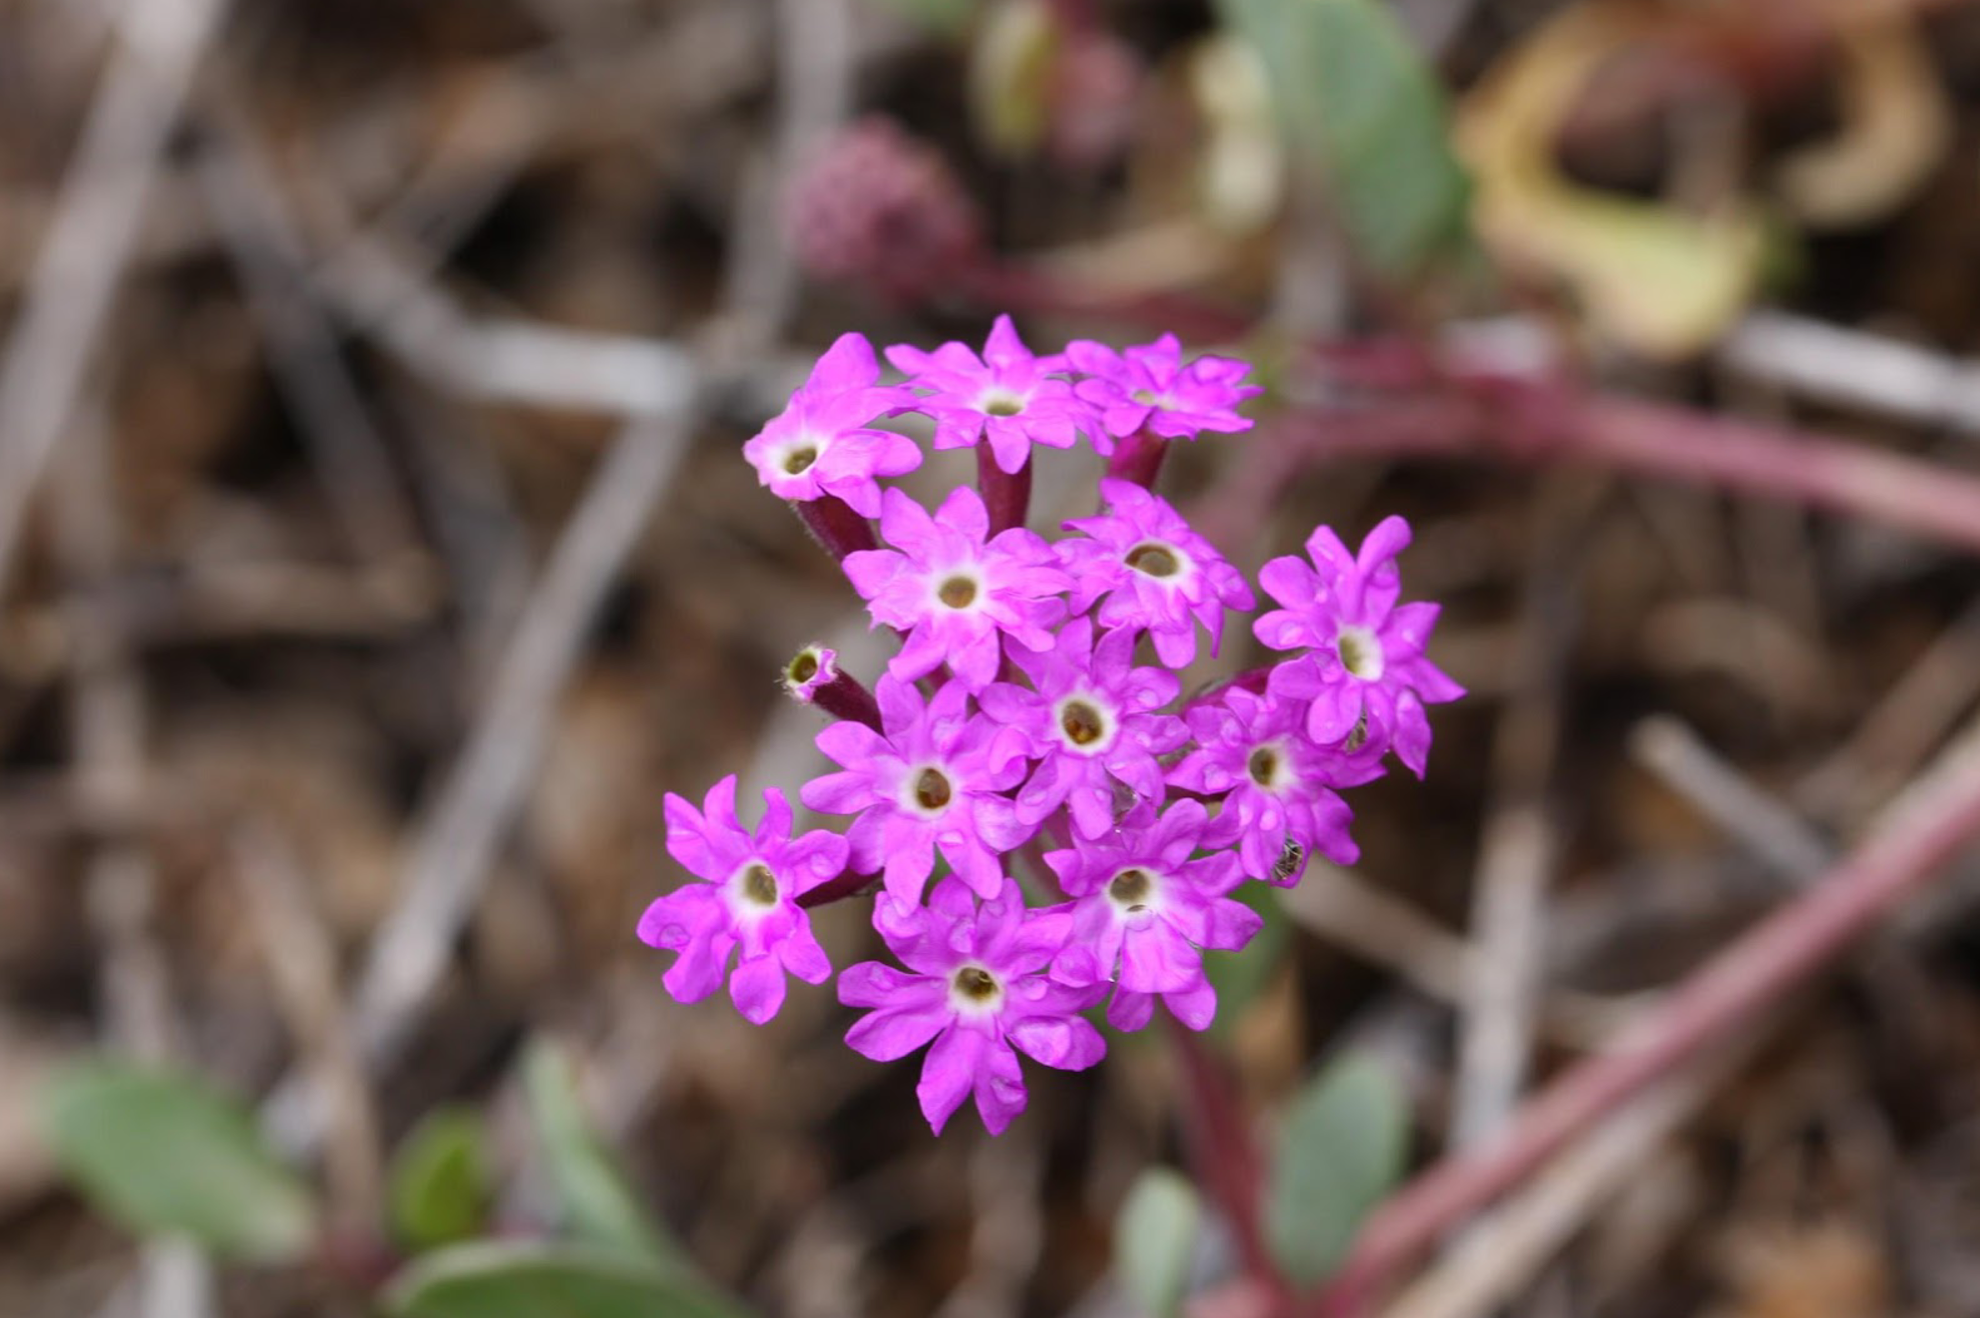
\includegraphics{protocols/images/img2.png}

}

\subcaption{\label{fig-umbellata}Abronia umbellata with chewing damage
to two corolla (one is completely chewed and one is partially chewed).
In this example, each floret would be scored for damage (2 damaged, 13
organs examined). Photo: Eric LoPresti.}

\end{minipage}%
%
\begin{minipage}{0.50\linewidth}

\centering{

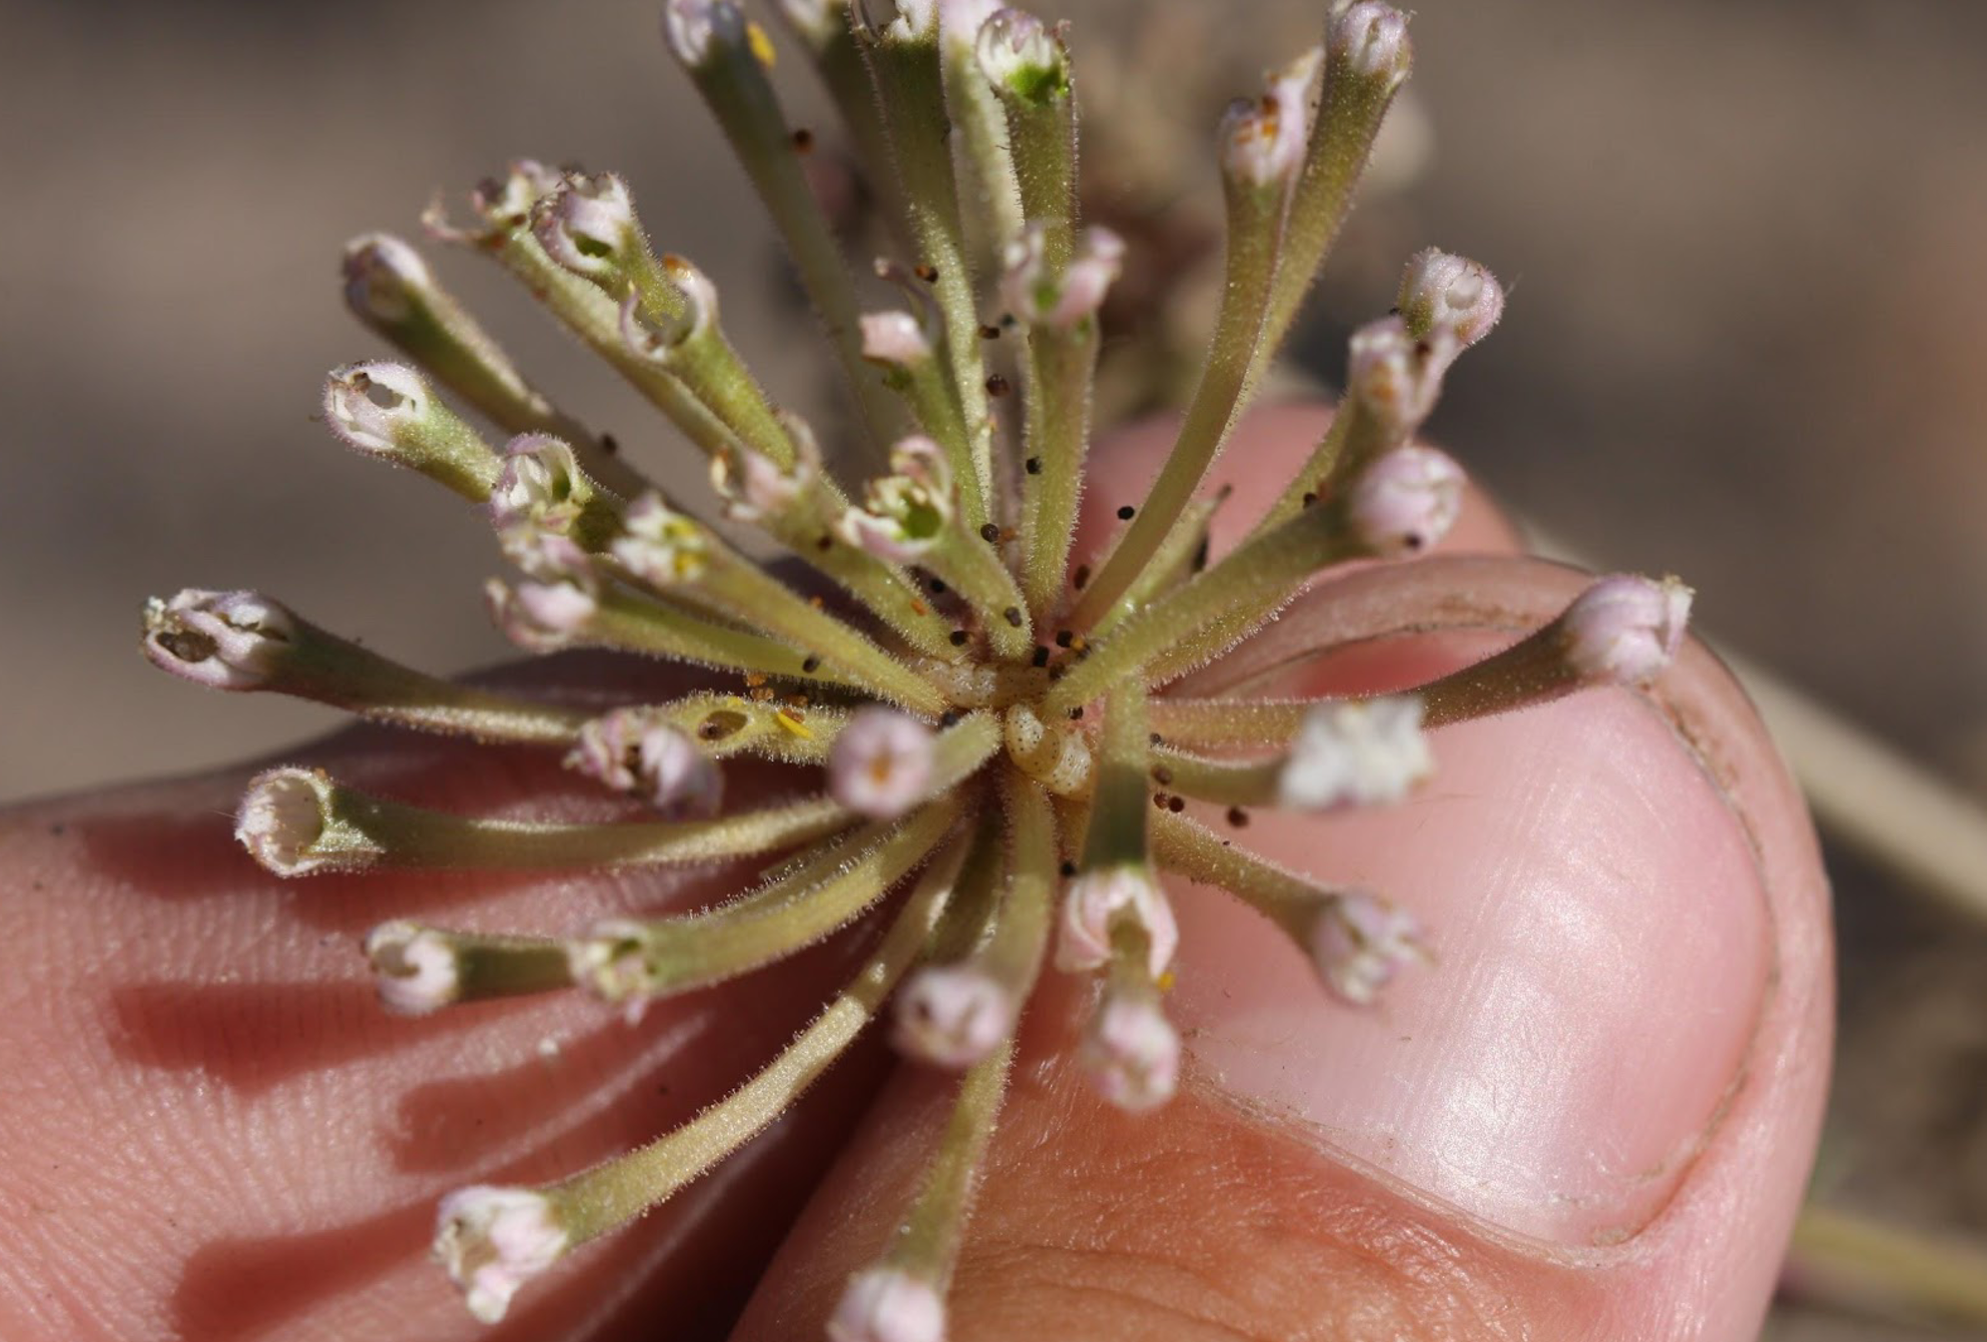
\includegraphics{protocols/images/img3.png}

}

\subcaption{\label{fig-turbinata}Abronia turbinata with damage and frass
from a moth caterpillar (Neogrotella macdunnoughi). Note chewing damage
to petals/corollas and caterpillars at base of florets. In this example,
each of 30 florets would be scored for damage. Photo: Eric LoPresti.}

\end{minipage}%

\end{figure}%

\begin{figure}

\centering{

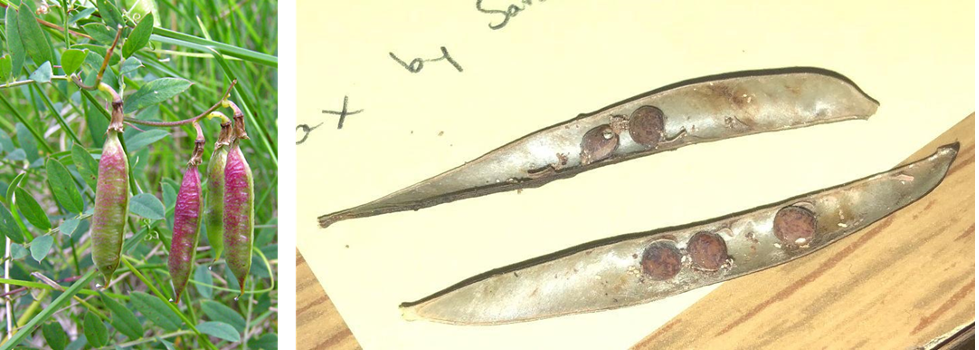
\includegraphics{protocols/images/img4.png}

}

\caption{\label{fig-americana}Vicia americana seed pod. Notice boring
holes in the upper-left seed and frass in the pod. In this example, each
of 30 seeds would be scored for damage. Photo: Phil Hahn.}

\end{figure}%

\begin{figure}

\begin{minipage}{0.50\linewidth}

\centering{

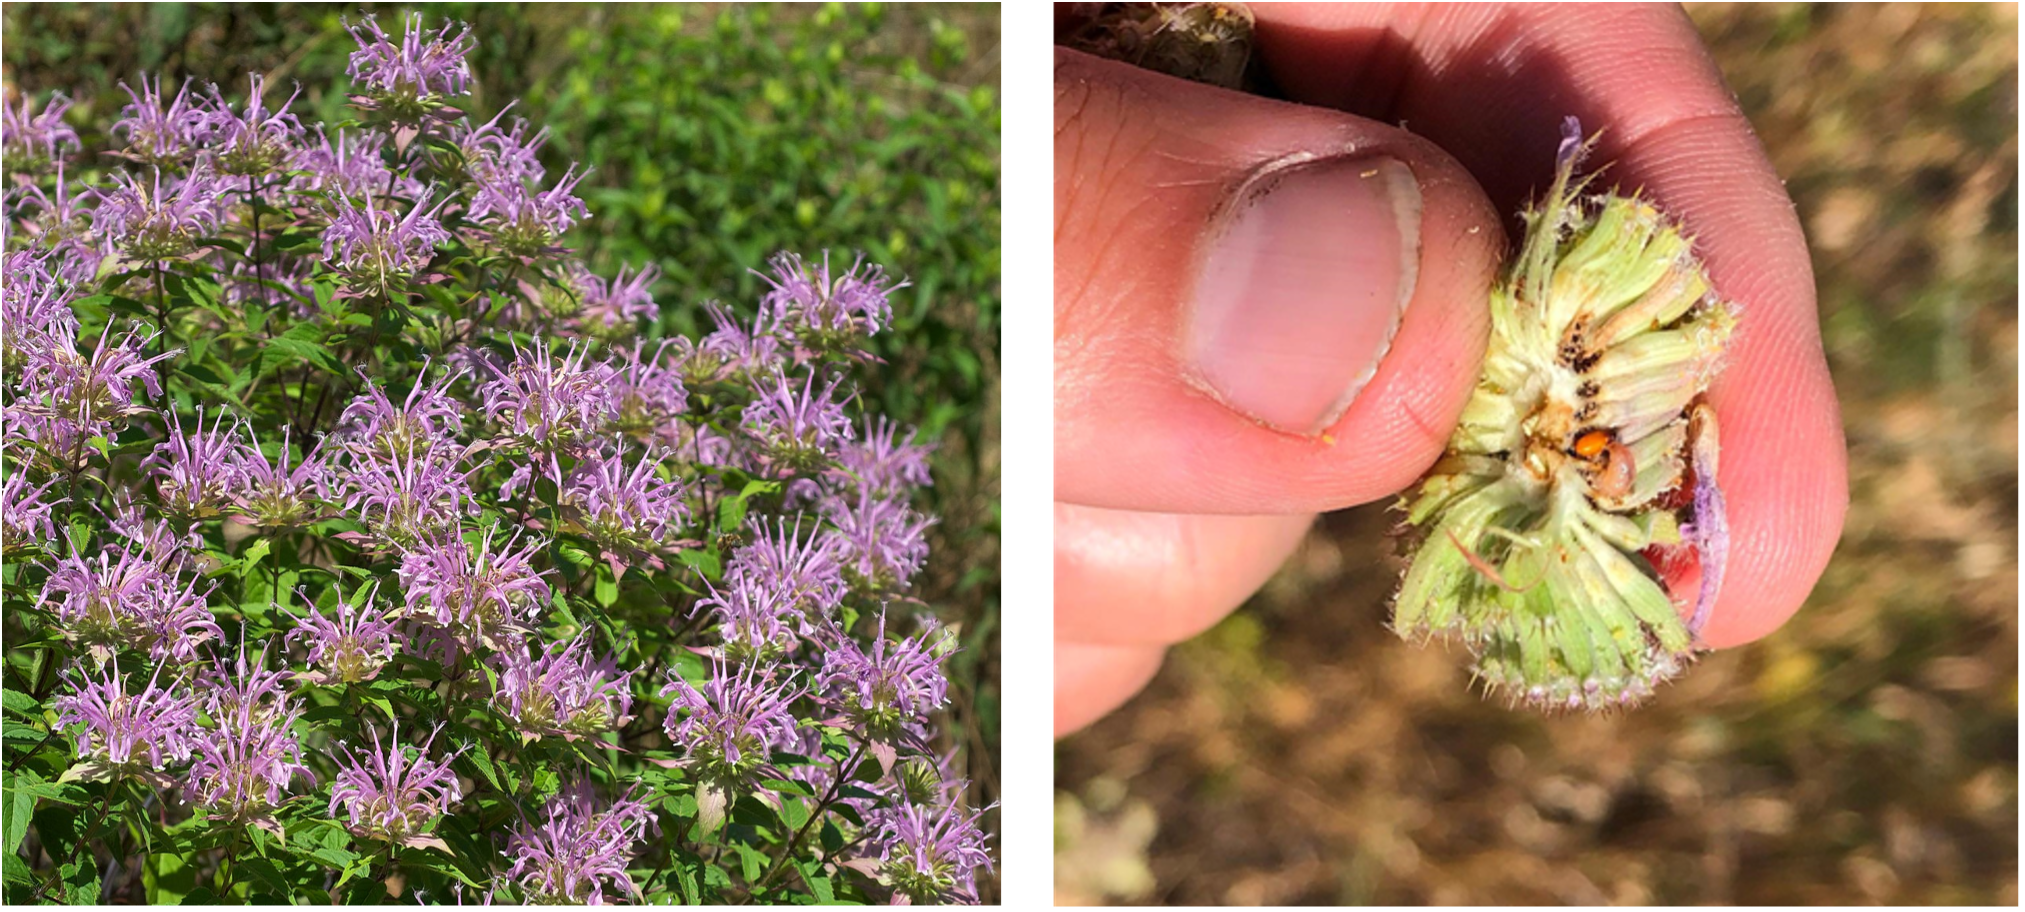
\includegraphics{protocols/images/img5.png}

}

\subcaption{\label{fig-fistulosa}Monarda fistulosa seed head ripped open
to reveal a weevil larvae. Notice the damage holes to the floral tubes.
In this example, each flower head would be recorded as damaged (or
undamaged) and ideally 30 flower heads would be assessed per plant.
Often this species does not produce 30 flowers per plant, so smaller
numbers would be acceptable. If most plants have fewer than 10 flowers,
this would not be a good population to survey for reproductive damage.
Photo: Phil Hahn. Lonicera fruit with chewing damage. In this example,
each of 30 fruits would be scored for damage. Photo: Susan Whitehead.}

\end{minipage}%
%
\begin{minipage}{0.50\linewidth}

\centering{

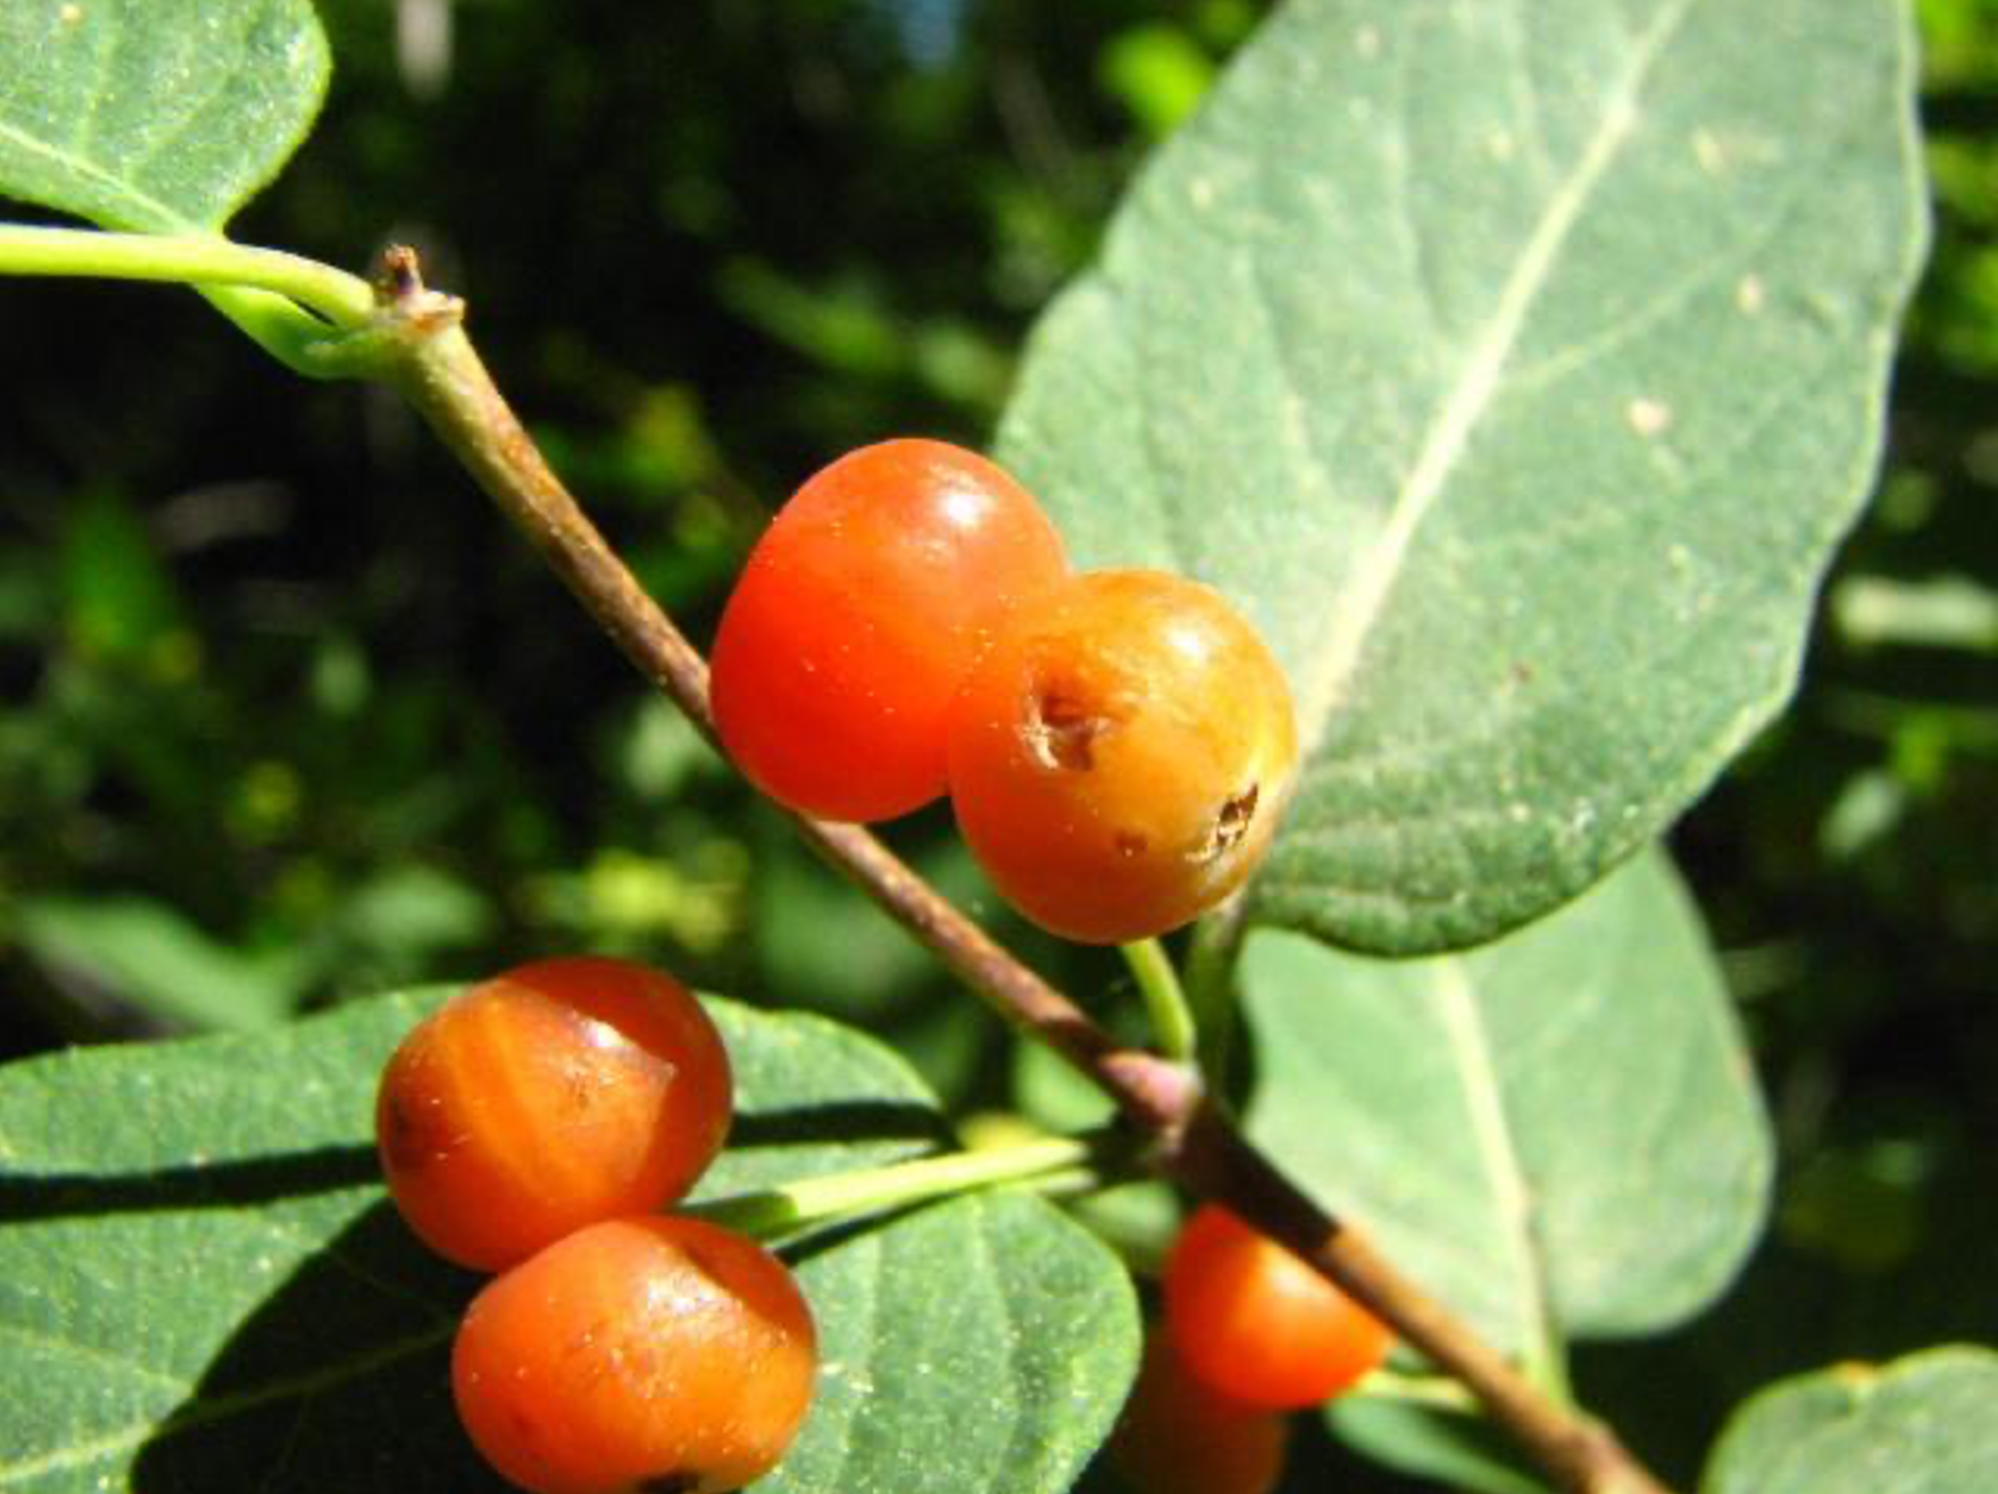
\includegraphics{protocols/images/img6.png}

}

\subcaption{\label{fig-lonicera}Lonicera fruit with piercing damage. In
this example, each of 30 fruits would be scored for damage. Photo: Susan
Whitehead. Aquilegia shockleyi with chewing damage to fruits (from
Heliothis phloxiphaga). In this example, each fruit could be scored for
damage, or each fruit could be opened and seeds could be counted (infer
missing, fully-consumed seeds from pod features). Photo: Eric LoPresti.}

\end{minipage}%

\end{figure}%

\chapter{Low Density/Abundance Plants}\label{sec-low_density}

\section{Overview}\label{overview-1}

This protocol outlines three methods for surveying sites where the focal
plant plant occurs at low density or low abundance. The Primary Protocol
was designed to work for many plant species, growth forms, and contexts,
but it requires sites with enough focal plants at a reasonably high
density for efficient random sampling using our transect/sub-transect
method. If the focal plants at your site are at very low density, then
sampling them with our primary method will be very time-consuming due to
the large distances between plants. If they are at low abundance, such
that there are fewer than about \textasciitilde90 plants in the site,
then it does not make sense to draw a random sample of 30 plants + 30
neighbors from such a small population. If none of the methods below
work well for your species and site, we encourage you to think of a
comparable alternative. Feel free to get in touch if you have questions.
Regardless of what you decide, please make sure to carefully document
your methods.

\section{Protocols}\label{protocols-1}

We provide three separate protocols for surveying sites with low density
and/or abundance of focal plants: (1) Comprehensive Patch Census, (2)
Walking Transect, (3) Comprehensive Census of Subset.

\subsection{Option 1 -- Comprehensive Patch
Census}\label{option-1-comprehensive-patch-census}

The best method, when feasible, is to census all of the individuals in a
patch. This will work when there is a well-defined patch with a
reasonable number of plants (e.g., \textless{} \textasciitilde90). If
this is possible, it is better in many ways than the Primary Protocol
because it describes the whole distribution of herbivory at the
site---there's no risk of missing the tails of the distribution if every
plant has been included! Also, depending on the context, this could be
faster than our Primary Protocol because setting up transects and
quadrats to randomly sample plants is time consuming. So comprehensively
examining all of a patch's 90 plants, for example, might be faster than
randomly sampling 60 plants (30 focal plants and their 30 neighbors)
from a larger population. For this method, we stress that you should
strive to survey every plant.

Record spatial information via one of two methods:

\begin{enumerate}
\def\labelenumi{\arabic{enumi})}
\item
  \textbf{Option 1A - Record GPS position of each plant: }If you do
  this, you will not need to record nearest neighbor information because
  we can reconstruct it (and more!) easily from the geographic
  coordinates. This of course means that you will need a GPS sensitive
  enough to differentiate the locations of your plants. If your plants
  are on average more than 2-3 m apart, then almost any modern GPS will
  be precise enough. If, however, your plants average less than
  \textasciitilde1 m apart, then you would need a very precise GPS to
  describe the relative locations accurately. If you don't have such a
  precise GPS (or if you don't like how slow a precise GPS can be), we
  recommend the second method.
\item
  \textbf{Option 1B - Relative spatial coordinates: } You can measure
  the relative coordinates of your plants using two tape measures or a
  tape measure and a meter stick. This sounds similar to the primary
  protocol but it's much quicker because you're not using the tapes to
  select plants, just to record their locations.

  \begin{itemize}
  \item
    Lay a tape measure through your patch. For each plant, record
    spatial coordinates as how far along the tape measure and how far
    from the tape measure. You can situate the tape either along the
    edge of the patch or through the middle of the patch.
  \item
    If your tape measure is through the middle of the patch, remember to
    record the distance left of the tape as negative and right of the
    tape as positive. The start of your tape will have the coordinate
    (0,0).
  \item
    After recording this information, follow the Primary Protocol as
    closely as possible
  \end{itemize}
\end{enumerate}

\textbf{Other useful information}

\begin{enumerate}
\def\labelenumi{\arabic{enumi}.}
\item
  Record \texttt{popDiameter1} and \texttt{popDiameter2} as the
  approximate extents of your patch/census area
\item
  For focal plant percent cover (\texttt{focalPlantCover}) and non-focal
  plant percent cover (\texttt{otherPlantCover}), please follow the
  Primary Protocol methods for estimating population density and
  calculating a quadrat radius size, if feasible. You can then center a
  quadrat on each focal plant in the census to define an area around
  each focal plant for recording focal and non-focal percent cover, as
  well as the number of focal plants in quadrat
  (\texttt{numPlantsinQuad}).
\item
  In comprehensive surveys the \textasciitilde60 plants will all be
  focal plants and there is no random selection; hence the nearest
  neighbors (all the ``.1'' plant IDs in datasheet template) become
  focal plants. As described above, a quadrat is centered around each
  plant and the three quadrat-level variables (\texttt{focalPlantCover},
  \texttt{otherPlantCover}, and \texttt{numPlantsinQuad}) are recorded
  for each plant. The nearest neighbor distance (\texttt{NNdist}) is
  still recorded, but since that neighbor is treated as a focal plant,
  please record the unique plantID of that nearest neighbor as well
  (e.g.~add \texttt{NNplantID} column as needed in datasheet).
\item
  If you cannot estimate population density (e.g., because your species
  is too sparse), then please pick an arbitrary quadrat radius. You can
  use that to define an area around each focal plant in your census for
  estimating percent cover variables. A 1-m radius might be a good
  choice for many plants, but go bigger for bigger plants. Remember to
  record your choice!
\end{enumerate}

\subsection{Option 2 -- Walking
Transect}\label{option-2-walking-transect}

Another alternative if you have widely dispersed plants that do not form
a well-defined patch (or the patch is too large for a comprehensive
search) is a walking transect.

\begin{enumerate}
\def\labelenumi{\arabic{enumi}.}
\item
  Randomly pick distances (e.g., paces) along a transect and from a
  transect.
\item
  Pace out the distance along the transect, then turn orthogonally to
  pace out the distance from the transect.
\item
  Survey the closest plant within some reasonable distance (if no plant
  is reasonably close, then go back to transect and keep going).
\item
  Repeat until you have 30 plants and 30 neighbors.
\end{enumerate}

This is similar to the Primary Protocol except pacing (rather than
measuring with a tape) can make large areas more feasible to survey.
Consider recording spatial coordinates for each plant, especially if
plants are far from your randomly identified points. And try to survey
neighbors for each plant.

\subsection{Option 3 -- Comprehensive Census of
Subset}\label{option-3-comprehensive-census-of-subset}

This method is similar to the comprehensive census of a patch (\#1
above), but it applies when there is no well-defined patch and
individuals are widely dispersed over a large area. There are two ways
to do this but for both of these methods, record spatial coordinates for
each plant and see other notes for method \#1 above.

\begin{enumerate}
\def\labelenumi{\arabic{enumi}.}
\item
  \textbf{Option 3A - Comprehensive survey of all plants along a
  transect: }With this method, you are doing a comprehensive survey of a
  linear subset of the whole population

  \begin{enumerate}
  \def\labelenumii{\alph{enumii}.}
  \item
    Start by randomly picking a transect starting point and direction
  \item
    Walk the transect and survey every plant that crosses your path
    \emph{or} every plant within a reasonable distance of your path
    (e.g., 2 m)
  \item
    Keep going until you get at least 60 plants
  \end{enumerate}
\item
  \textbf{Option 3B: Comprehensive survey radiating out from a random
  starting point within a population. } With this method, you are doing
  a comprehensive survey of a roughly circular (or blobby) area within
  the whole population. The cons of this approach are that if your
  plants are close together there could be high spatial autocorrelation
  such that you fail to capture the range of herbivory levels in the
  population. Of course, this is always a risk; it's just especially
  acute when the sampling extent is an arbitrary area rather than a
  biologically significant ``patch'\,'.

  \begin{enumerate}
  \def\labelenumii{\alph{enumii}.}
  \tightlist
  \item
    Explore outwards from your random starting point, surveying every
    plant you encounter until you get to at least 60 plants. \emph{We do
    not recommend doing this unless your plants truly are all widely
    dispersed.}
  \end{enumerate}
\end{enumerate}

\chapter{Cacti \& Succulents}\label{sec-succulents}

\section{Overview}\label{overview-2}

This document discusses issues relevant for quantifying herbivory on
cacti and outlines a hopefully widely applicable protocol for doing so.
The protocol is designed for cacti that have many jointed segments, but
we also discuss ways to modify the protocol for other architectural
types. Although we focus on cacti, we think this document will also be
helpful for other succulents. Please share feedback, particularly ways
we can make this widely useful.

\textbf{Unique Context: } With regard to quantifying herbivore damage,
cacti are special: (a) they are architecturally unique, (b)
architecturally distinct from each other, and (c) much of the herbivory
is surficial (there are few ``edges'' to bite!) and (d) since units are
not lost, damage can persist for decades. Any census method needs to
take these factors into account.

\section{Sampling Issues within Architectural
Categories}\label{sampling-issues-within-architectural-categories}

Cacti can be thought to consist of one or more (usually spiny) tubes
with flowers usually located at the tip of the tube -- that's what they
have in common -- with these tubes having a diversity of spatial
relationships to each other -- that's what makes them different from
each other. There are at least five categories, each with its own
herbivory sampling issues Single, unbranched tube stuck in the ground
(e.g., in the American Southwest, a barrel or a pincushion cactus). As
they age, they get taller and wider, but they never branch or clone. If
there is a cluster, they are genetically different from each other (I am
almost sure, JB).

Entire structure should be scrutinized for herbivore damage. When these
cacti form a cluster, they should be categorized as multiple individuals
rather than as a single individual.

Set of unbranched tubes connected underground (e.g., a hedgehog cactus
(small), or a senita or organ pipe cactus (large)). They add units as
they age.

Either the whole thing can be scrutinized for damage, or a subset of
units could be (please make a note of which path you chose). If there
are not that many units, full sampling is possible. However, some of
these cacti get very tall. Since much damage seems to accrue at tube
tips, one really should look at the entire length. Tube that starts to
branch above the ground as it ages (e.g., a saguaro cactus).

Same method as \#2 (again, please make a note of whether you examined
the whole plant or a subset of units).

Large set of tubes connected at distinct joints (e.g., a cholla cactus).
New tubes are added as the plant ages.

Subsampling within individuals will usually be necessary because
individuals often have many tubes. Our protocol below, which is focused
on cacti with many joints, describes a method for subsampling up to 20
joints per plant.

Large set of tubes connected at distinct joints but flattened into
pancakes (e.g., a prickly pear cactus). New tubes are added as the plant
ages.

Same method as \#4.

\section{Expected Types of Herbivory}\label{expected-types-of-herbivory}

Bites that remove chunks of flesh.

This is quite obvious for the fifth category of cacti (flattened pads),
because the pads have smooth edges that will be disrupted by this type
of herbivory. So if this category is being surveyed, special attention
should be paid to the edges of pads. I am not sure if it will be
evident, or at least common, for any other category: only this category
consists of units with ``edges''. I suspect that other cactus-feeders
that take out chunks of flesh concentrate on the youngest tissue (new
units and the tips of existing units), and this suggests important
sampling rules: young units should be sampled, as well as tips of
existing units (which, unfortunately, might be very high in the air).
Some large beetles burrow into cactus flesh, but (based on my knowledge
of barrel cactus) these individuals rapidly die, so this sort of damage
is unlikely to persist

Scarring of the surface of the cactus.

It can be very hard to know what causes this -- some of this damage may
be attributable to herbivores, but some might be fungal or bacterial
attack. It is worth taking photos of the damage and trying to figure out
the culprit. Damage left by various small herbivores on various cactus
species has been described in the literature and it may be worth making
a photo album for later identification.

Colonies of sucking insects.

In particular, cochineal bugs live in colonies and are exciting to see.
They are covered with a messy white wax. At least in the desert
Southwest, cochineal are primarily found on introduced Opuntia
ficus-indica. However, there are small colonies on Opuntia englemanii as
well that should be watched out for.

\section{Other Notes About Cacti}\label{other-notes-about-cacti}

Some genera have species with extrafloral nectaries (EFNs). Most (not
all) barrel cacti have them, and I believe all columnar cacti (senita,
organ pipe, saguaro), prickly pear, and cholla do. On the other hand, I
don't know of any hedgehog or pincushion cacti that have them. Ant
attraction to extrafloral nectaries may reduce herbivore attack, though
field evidence for this has varied across cactus species, and ants are
often surprisingly rare. Most EFN-bearing cacti only secrete nectar when
there is new vegetative growth, buds, flowers, and early fruit present,
but some (such as the fishhook barrel cactus abundant in Tucson) secrete
it year-round.

It seems likely that the newest, tenderest units (particularly in
categories 4 and 5 cacti) are particularly likely to be attacked.

The buds and young fruits of some cacti get very heavily attacked, and
these should be included by counting damaged and undamaged units and
recording the data separately (see Reproductive Damage Protocol).

\section{Protocol}\label{protocol-1}

We designed this with prickly pear (Opuntia spp.) in mind, but it should
work essentially the same way for other cacti with many jointed tubes
(e.g., cholla Cylindropuntia spp.). Modifications will be necessary for
some cacti.

The gist of the protocol involves following the Primary Protocol except
for a subsampling of leaves and reproductive units (if present) within
plants. We suggest taking both this protocol and the Primary Protocol
with you in the field.

\section{Pre-Census Tasks}\label{pre-census-tasks}

Pick a species to census.

Choose a site, ideally with at least 90 well-defined individuals that
you can randomly sample using the HerbVar Primary Protocol. If your site
has fewer than \textasciitilde90 individuals or has very widely spaced
individuals, we suggest following methods from our document on Surveying
low-density/low-abundance sites.

Decide on a maximum number of pads per plant to census.

We recommend focusing only on young cactus pads. But you should decide
if this will do a good job representing the plant-herbivore interaction
and distribution of herbivory for your species. By young pads we mean
those that are final joints, i.e., that don't have another pad growing
out of them. Problems with older pads include: Older pads can be many
years old, thus integrating herbivory over a much longer time than
happens for other plant species in HerbVar (few plants hold leaves as
long as cacti hold their pads)

Practically, it's very hard to determine and quantify what is herbivory
vs physical damage on older pads Physically, it can be hard and
dangerous to access older pads on spiny plants!

If you think focusing on young pads will not be good for your species,
then please modify the protocol to include older pads. Take detailed
notes.

Ideally, investigate the major types of damage you may see, potentially
making a cheat sheet of photos. See how long the protocol outlined below
would take, then modify as necessary.

Please take detailed notes on any modifications made

\section{Census}\label{census}

Record site characteristics (e.g., date, site, plant ID, etc.)

Decide how you will define an individual plant. Past populations we
surveyed had many very large clumps of pads that were almost certainly
one plant individual, though not all connections were visible
aboveground. In most cases, the clumps were discrete enough that we were
confident each clump was one individual with below ground connections.

See above discussion of architectural categories of cacti/succulents

If you have a site with \textgreater90 plant individuals, follow the
Primary Protocol from the beginning until you have your first plant for
herbivory estimation. Briefly:

Pick transect and subtransect distances that will encompass your site
and lay the transect through the site. Estimate the density of plants in
the population.

Use the estimated plant density to calculate a quadrat radius to use for
the survey.

Randomly generate x,y points, visit them, and set up a quadrat centered
on each random point, selecting 1 plant randomly within each quadrat.
See the Primary Protocol for more detail.

Once the first plant is selected, survey it for herbivory. For
vegetative herbivory, we recommend focusing only on terminal pads (see
\#4 above). Terminal pads are those at the end of a branching structure,
without another pad growing out of them. Also, focus only on the visible
surfaces of pads because moving spiny pads safely is difficult and time
consuming! Record herbivory from all organisms in one column and
herbivory you are certain was just from insects in a second column. We
found it was difficult to distinguish insect herbivory from vertebrate
herbivory, so we usually recorded ``totalHerb'' Occasionally it was
clear some herbivory was just from insects, so then we used the
``insectHerb'' column to indicate what percent was definitely from
insects. There are 3-4 herbivory estimation steps, depending if your
plant has reproductive organs: Quickly scan all of the terminal pads
across the entire plant and visually estimate percent herbivory. This is
a quick estimate, but it's important to scan the whole plant because
herbivory can be patchy within plants.

Randomly select 20 of the terminal pads. Record the number of pads you
examined and the number with any herbivory present. If there are fewer
than 20 pads on the plant, then do all pads.

Randomly select 10 terminal pads, and record a visual estimate of the
percent herbivory on each pad, resulting in 10 numbers (one number for
each of the 10 pads). We estimated percent herbivory as surface area
removed on the visible faces of paddles (as opposed to volume or
doubling the area for holes that went entirely through a paddle).

If your plant has reproductive organs, please randomly (arbitrarily)
select up to 20 units of one type (e.g., flowers or fruits) and record
the number of units you examined and the number that were damaged
(\textgreater0.5\%). Please see the Reproductive Damage Protocol for
more information. You will need to add columns to the HerbVar Template
Datasheet to accommodate this.

Note presence of pathogens.

\chapter{Trees}\label{sec-tree}

Protocol -- Tree Seedlings \& Saplings Protocol -- Mature Trees
Selecting Leaves for Herbivory Estimates

\section{Overview}\label{overview-3}

Mature trees, though harder to study than smaller plants, are a key
plant growth-form that could have their own characteristic patterns of
interactions with herbivores. Therefore, we want to include enough
surveys of mature trees in HerbVar's global sampling to allow us to
compare patterns between trees and other growth forms. It is also
important to include mature trees because there may be major shifts in
tree-herbivore interactions with tree ontogeny, from seedling to sapling
and sapling to adult.

\section{Objectives}\label{objectives-1}

Provide a protocol for sampling mature trees. Collaborators who do not
have a special interest in working with mature trees should restrict
their surveys to individuals ≤ 2 m height (seedlings and saplings). That
is, survey tree species, but focus on seedlings and saplings.
Seedling-sapling surveys won't be representative of all the individuals
in a population of a tree species, but these are key stages in tree
ontogeny---perhaps the stages in which herbivory is most influential. We
are taking a two pronged approach to including tree species in HerbVar.

\section{Protocol -- Tree Seedlings \&
Saplings}\label{protocol-tree-seedlings-saplings}

Follow the Primary Protocol. This includes (but isn't limited to) the
following data:

\begin{enumerate}
\def\labelenumi{\arabic{enumi}.}
\tightlist
\item
  Leaf-level percent herbivory estimates for 10 randomly selected leaves
\item
  Counts of presence/absence of herbivory for up to 60 leaves per plant
\item
  A whole-plant visual estimate of herbivory
\item
  And of course please record the number of galls, mines, and other
  discrete damage types from sessile herbivores
\end{enumerate}

Please note in the metadata that you surveyed only immature individuals
(≤ 2 m) at your site. Such a note can be complemented by recording the
height of the individuals in the plantSize columns

\section{Protocol -- Mature Trees}\label{protocol-mature-trees}

Follow the Primary Protocol \& Site Selection Protocol to pick a site,
set up a transect, and randomly select focal trees or quadrats. Many
tree species cover huge geographic areas, making it unreasonable to
survey an entire ``population'' or define a discrete study ``site.'' If
you are working with a widespread species, it is fine to choose a
``representative'' study area, which actually might just be a small part
of a large stand of trees.

Once you have selected a representative study area, you will need to
randomly select 30 trees to survey (plus their nearest conspecific
neighbors). There are many ways to do this. Here are three methods in
somewhat decreasing order of amount of work and rigor:

Follow the Primary Protocol exactly, establishing a transect, selecting
30 points randomly (distance along main transect and distance from main
transect), and using a circular quadrat at each point to randomly select
1 individual of the tree species within the quadrat (as in the Primary
Protocol). Survey each selected tree and its nearest neighbor.

Follow the Primary Protocol except skip the circular quadrat step, which
could need to be prohibitively large in some tree populations: Establish
a transect and randomly select 30 points (distance along main transect
and distance from main transect). Then select and survey the individual
nearest to each random point (plus nearest neighbor).

For trees that are at low density or low abundance, please consult our
Low Density Protocol to select trees. For low-abundance plants, we
recommend surveying every plant within some area. Take GPS coordinates
for each plant. Try to get as close to 60 plants as possible. If you are
taking GPS coordinates for each plant, then you do not need to measure
distances to nearest neighbors because we can measure spatial
relationships using the GPS data.

However you select trees, please make sure to take detailed notes on
what you did

Note that some of the trees you select may be seedlings or saplings. We
recommend doing whichever individual you randomly select, regardless of
its age. This should yield a representative sample of all individuals at
the site, across age classes

Randomly select 30 leaves for quantitative estimates of percent
herbivory on each of the 30 leaves See Primary Protocol and Damage
Estimation Training Document for guidelines on quantifying percent
herbivory per leaf

Please also record the number of galls, mines, and other discrete damage
types. Note that mines should be included both in percent damage
(because they represent damaged surface area) and as counts.

Randomly select an additional 30 leaves to score for presence/absence of
herbivory. Record the number out of 30 with herbivory.

Do not worry about estimating herbivory at the whole-plant scale for
mature trees; we will estimate this using the 30 presence/absence leaves
and the 30 percent herbivory leaves

\section{Selecting Leaves for Herbivory
Estimates}\label{selecting-leaves-for-herbivory-estimates}

Trees\ldots{} are tall, and we will not be able to reach top branches.
We will therefore focus on low branches that can be reached from the
ground with a pole pruner, and sample from multiple places around the
circumference (see below). We provide some guidelines below, but you
should choose an approach that makes sense for you and your species.
Remember that we are trying to acquire a random subsample of all leaves
on the tree; this means avoiding any preference for/against particular
leaves (e.g., young vs old).

\begin{figure}

\centering{

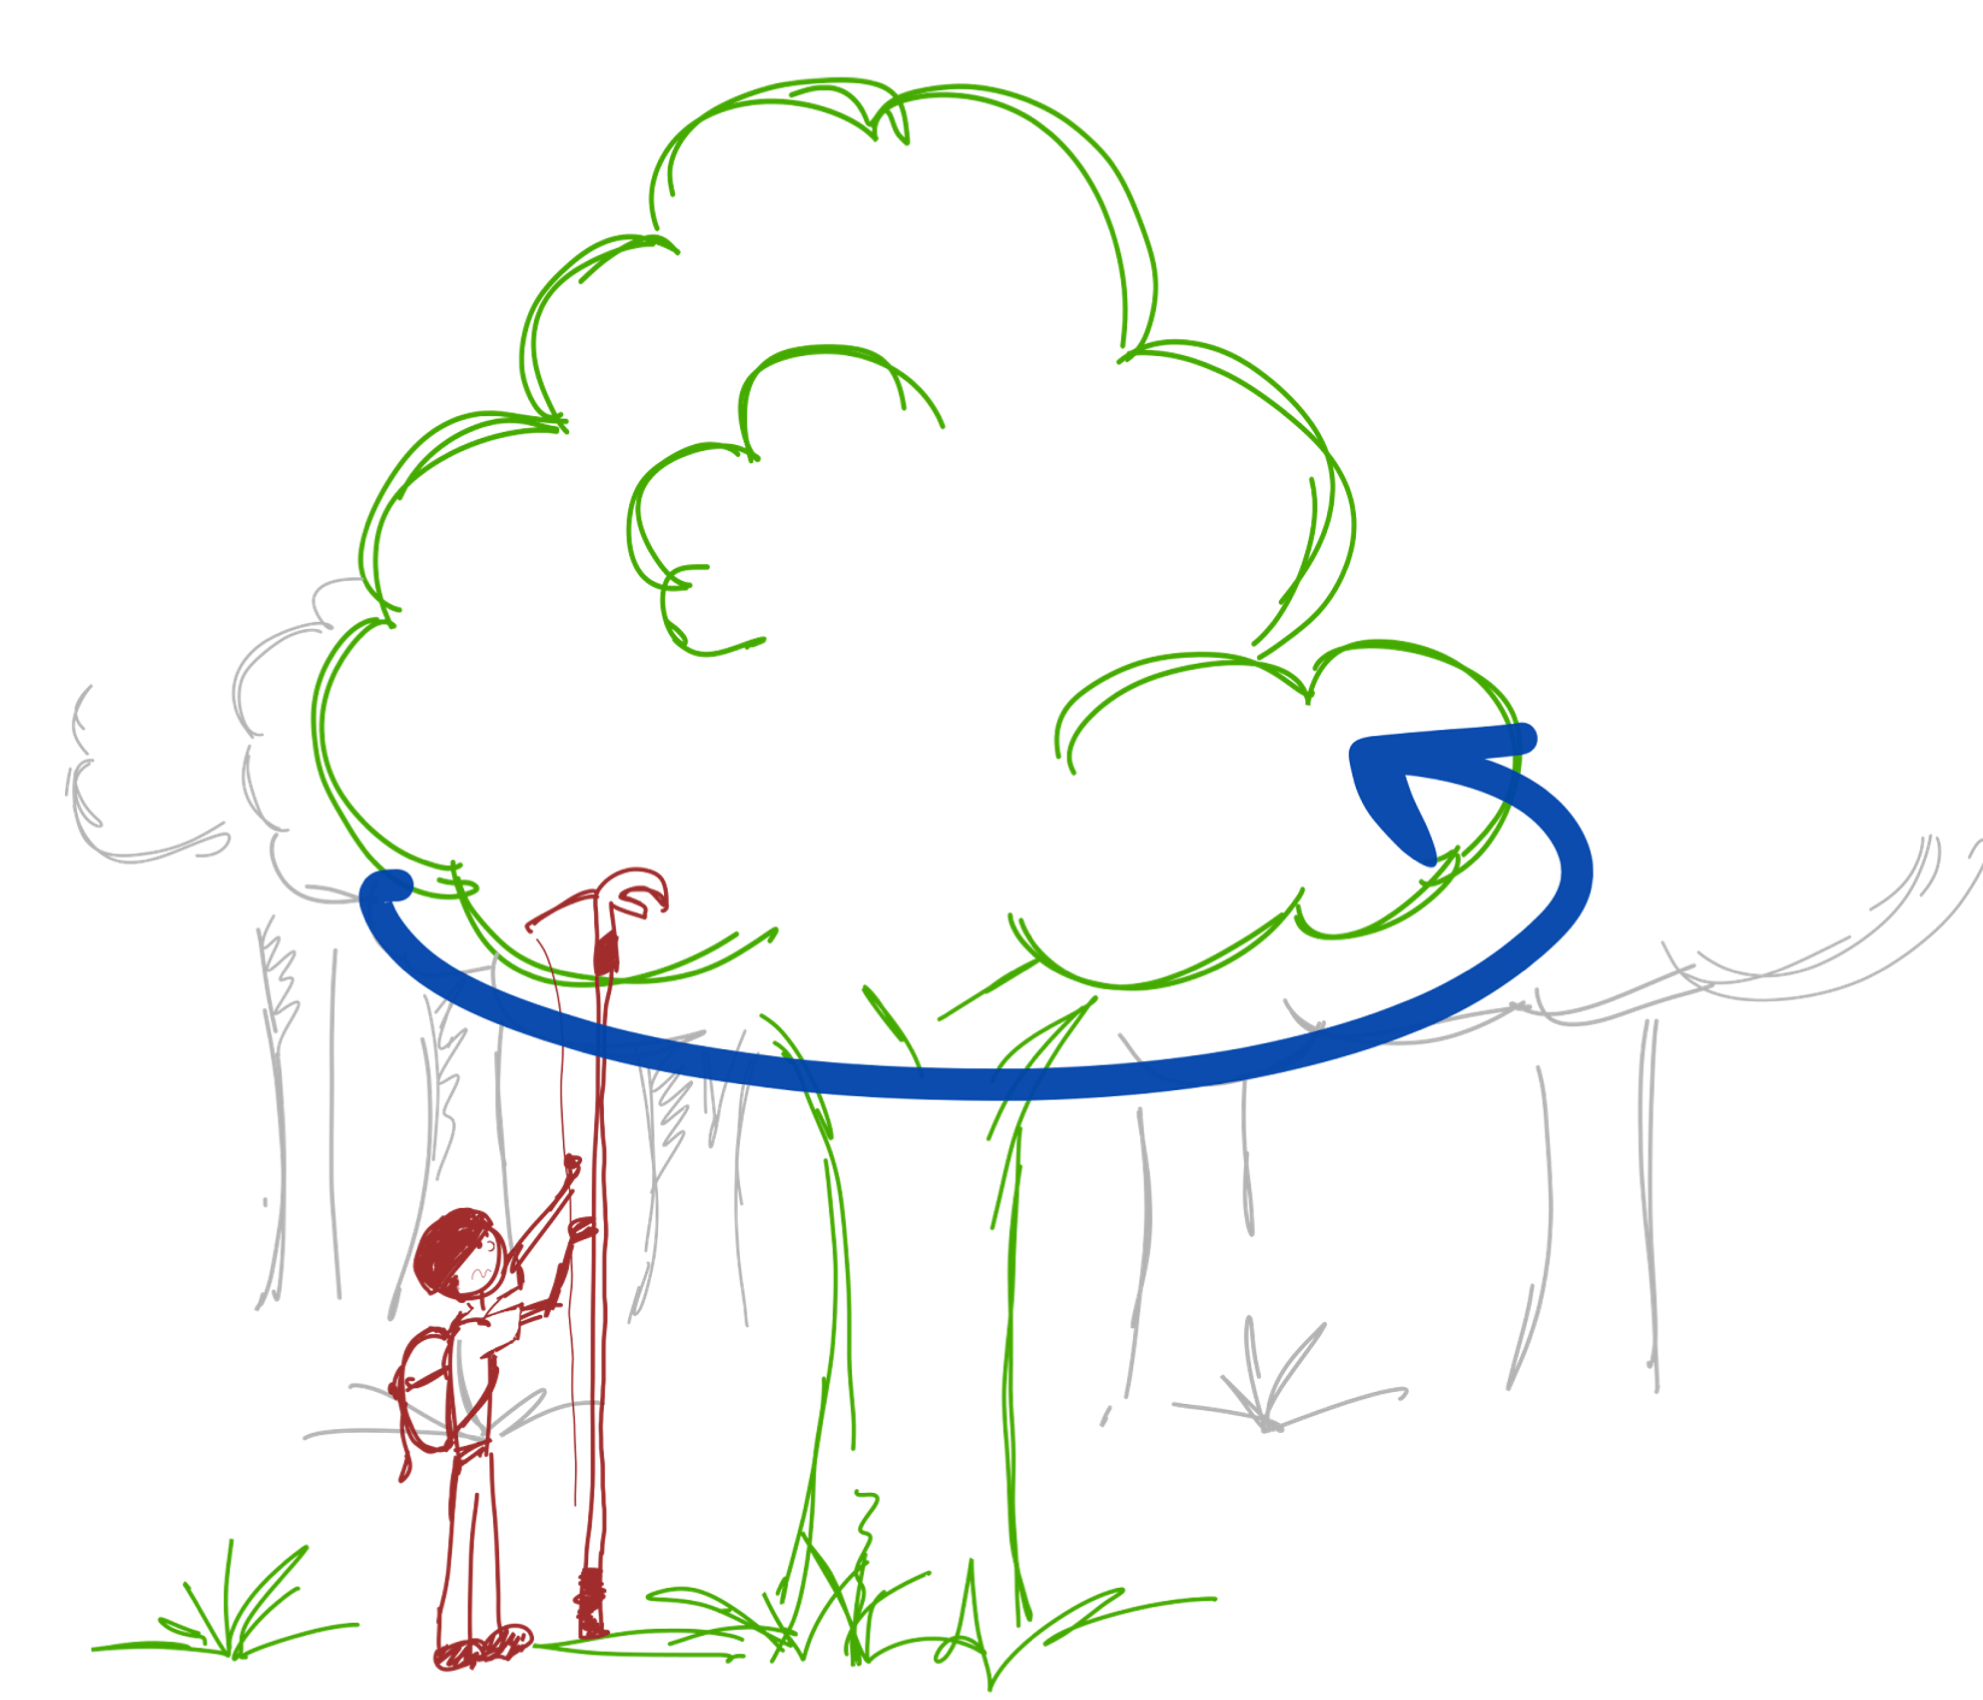
\includegraphics{protocols/images/img17.png}

}

\caption{\label{fig-tree}Focus on low branches that can be reached from
the ground with a pole pruner, and sample from multiple places around
the circumference}

\end{figure}%

Ideally, leaves will be sampled in proportion to their frequency on the
tree. Here are two alternate methods for selecting random (or at least
haphazard) leaves

\textbf{The easiest method:} if it would work for your trees, is to
close your eyes, point at the tree, open your eyes, and take the leaf
you were pointing at (``Ian's nose pointing method'' in the Damage
Estimation Training Document).

\textbf{Perhaps the most rigorous but most time-consuming method: } is
to haphazardly strip several times as many leaves as you need (e.g.,
\textgreater200 leaves). Place leaves individually into a large bag. Mix
them. Close your eyes and draw 30 leaves for percent herbivory and 30
leaves for presence/absence of herbivory.

\chapter{Rhizomatous Geophytes}\label{sec-rhizo}

Clonal plants present an interesting challenge and opportunity within
the HerbVar Network. From a question-based perspective, we may be able
to compare patterns of herbivory variability between clonal vs
non-clonal plant species. These different modes of reproduction may
confer different levels of genetic and phenotypic diversity within plant
populations (Sapir and Shmida 2002, Wilson et al. 2016) , which could
affect patterns of herbivory. However, from a practical perspective,
quantifying herbivory among plant `individuals' is a challenge in these
systems (i.e., what constitutes an `individual'?).

\textbf{Objectives:} Provide a protocol for surveying herbivory on a
rhizomatous plant species that meets two conditions: (1) it is feasible
to determine what constitutes a genet by examining rhizomatous
connections, and (2) genets are small enough at your study site that you
could feasibly survey 30 genets and their nearest neighbors and estimate
herbivory on each genet.

\section{Background}\label{background}

In semi-arid and arid climates, a considerably large number of plant
species are rhizomatous geophytes. Their major characteristic is that
they grow as patches of individuals, forming either dense (phalanx) or
sparse (guerrilla) mats of individual ramets, each visible as a single
leaf fan, and all connected through below-ground rhizomes and/or
above-ground stolons into one plant (genet) (terms following Harper
1977, Herben and Klimešová 2020). The extent of clonal growth defines
the spread of the genet, and is on a continuous scale of density
(Vallejo-Marín et al. 2010). See Figure 1 for examples of two density
levels of genets in irises.

\section{Protocol -- Rhizomatous
Geophytes}\label{protocol-rhizomatous-geophytes}

\begin{enumerate}
\def\labelenumi{\arabic{enumi}.}
\item
  When first starting this for a new species or at a new site, we
  suggest spending time investigating what constitutes a genet. Follow
  rhizome connections from ramet to ramet to get a sense of what a
  single genet looks like before following the rest of this protocol.
\item
  Follow the Primary Protocol \& Site Selection Protocol to pick a site,
  set up a transect, and randomly select focal quadrats' locations
\end{enumerate}

\subsection{Calculate a custom radius for circular
quadrats}\label{calculate-a-custom-radius-for-circular-quadrats}

Estimate mean density of genets per square meter by counting the number
of plants in 1 m2 at 10 random locations within the site

\begin{itemize}
\tightlist
\item
  If genet area (clone/genet diameter) is \textgreater1 m and/or
  distances between genets are apparently irregular (that is, secondary
  dispersion of plants within population is patchy), count the number of
  genets in 1 m2 every 5 meters along a 50 m transect.
\item
  If a quadrat has \textgreater0 focal plants, randomly choose 1 of the
  genets to survey and record the following data:
\end{itemize}

\subsection{Genet life stage: seedling, vegetative,
reproductive}\label{genet-life-stage-seedling-vegetative-reproductive}

Genet size, measured as the height of the tallest leaf for plants in
vegetative stage, or height of the taller flower for plants in
reproductive stage. Record which metric you used in the
``plantSizeMetric'' column

\subsection{Herbivore damage in one of 3
ways:}\label{herbivore-damage-in-one-of-3-ways}

\begin{enumerate}
\def\labelenumi{\arabic{enumi}.}
\tightlist
\item
  Total number of leaf fans (ramets)
\end{enumerate}

\begin{itemize}
\item
  For genets with \textgreater100 ramets, write ``100'' and make a note
  that your estimate was capped at 100 Estimated percent damage across
  the whole genet. Visually scan all the green areas of all ramets and
  all leaves, and estimate the percentage of damage.
\item
  If the plant has \textless10 ramets, sample all ramets. From each
  chosen ramet, pick the 2nd or 3rd leaf from top and estimate percent
  herbivory. These leaves are putatively in the same developmental stage
  and are the same age, thus exposed to herbivory for equal time
\end{itemize}

Note that tip of the leaf may be dry due to climate fluctuations in the
arid regions. This area of dry leaf counts as leaf area, but not as
herbivory damage

\begin{enumerate}
\def\labelenumi{\arabic{enumi}.}
\setcounter{enumi}{1}
\item
  If a quadrat has 0 focal plants, record a 0 and move to the next
  quadrat
\item
  Record the same data for the first nearest conspecific neighbor (of a
  different genet) that you recorded for the focal plant.
\item
  Continue visiting randomly select points until ≥ 30 focal genets and
  30 nearest neighbor genets have been surveyed
\end{enumerate}

\begin{figure}

\centering{

\includegraphics{protocols/images/img18.png}

}

\caption{\label{fig-rhizo}Top left: Dense (``phalanx type'') genet of
Iris atrofusca; Top right: Sparse (``guerrilla type'') genet of Iris
bismarckiana; Bottom left: Compact rhizome of Iris atrofusca (this one
has \textasciitilde4 leaf-fan ramets); Bottom right: Stolons connecting
ramets of Iris bismarckiana.}

\end{figure}%

\chapter{Herbivores, Mines, and Galls}\label{sec-herbivore}

\section{Overview}\label{overview-4}

Though a lower priority than the damage data, these data will permit us
to pilot some more mechanistic questions about the distribution of
herbivory (e.g.~spatial aggregation of herbivores). So far, observers
have been recording as much herbivore data as they can via a quick
visual survey; however, this may not be feasible for all observers or
systems.

\begin{tcolorbox}[enhanced jigsaw, opacityback=0, colback=white, breakable, toprule=.15mm, title=\textcolor{quarto-callout-important-color}{\faExclamation}\hspace{0.5em}{Important}, left=2mm, coltitle=black, bottomrule=.15mm, arc=.35mm, leftrule=.75mm, rightrule=.15mm, bottomtitle=1mm, toptitle=1mm, colframe=quarto-callout-important-color-frame, colbacktitle=quarto-callout-important-color!10!white, opacitybacktitle=0.6, titlerule=0mm]

For all plants, record the number of leaf mines and galls on the entire
plant. If there are too many to count individually, please estimate (for
example, by counting the number present on some module of the plant
{[}e.g., a branch{]} and multiply by the number of modules).

Separate from counting mines and galls, please also collect insect
herbivore data if you are confident in insect ID (see below for
specifics).

\end{tcolorbox}

\section{Protocol}\label{protocol-2}

\subsection{\texorpdfstring{\textbf{Deciding whether to sample ``core''
herbivores.}}{Deciding whether to sample ``core'' herbivores.}}\label{deciding-whether-to-sample-core-herbivores.}

Please use the following questions to help you decide whether to sample
``core'' herbivores.

\begin{enumerate}
\def\labelenumi{\arabic{enumi}.}
\item
  \textbf{Are you comfortable distinguishing the following 5 groups of
  herbivores? }If not, prioritize another herbivory survey (see the
  Primary Protocol).

  \begin{itemize}
  \item
    Grasshoppers/crickets/katydids (Orthoptera).
  \item
    Caterpillar-like larvae (i.e., eruciform larvae).
    \textbf{\emph{Note}: }this includes moth/butterfly caterpillars,
    sawfly (Hymenoptera: Symphyta) larvae, and some beetle larvae but
    does not include larval true flies (i.e., maggots)
  \item
    Aphids (Aphididae)
  \item
    Hoppers (Hemiptera: Auchenorrhyncha). This includes planthoppers
    (Fulgoromorpha), leafhoppers (Cicadellidae/Cercopidae), treehoppers
    (Membracidae), \& cicadas (Cicadidae). If you are confident, you may
    also identify non-''hopper'' Auchenorrhynchans in the column
    provided in the template Excel file
  \item
    Non-Aphid Sternorrhynchans. This includes whiteflies, scale insects,
    and mealybugs
  \end{itemize}
\item
  \textbf{Are you confident that you can visually detect the herbivores
  on the selected plant species,} considering the complexity of plant
  structure? If not, prioritize another herbivory survey (see the
  Primary Protocol). If you have the ability to sample herbivores in
  another way (e.g., a beat-sheet) and feel excited about this, feel
  free -- but be judicious of the added time required for sorting
  through a loaded beat-sheet!
\item
  \textbf{Could you do another herbivory survey with the time required
  to conduct an herbivore survey?} If yes, prioritize another herbivory
  survey (see the Primary Protocol). If not, please collect herbivore
  data!
\end{enumerate}

\subsection{Sampling insects beyond ``core''
herbivores.}\label{sampling-insects-beyond-core-herbivores.}

\begin{enumerate}
\def\labelenumi{\arabic{enumi}.}
\item
  In an effort to standardize the insect data we have included 5
  groupings to use for tallying herbivores. This is to avoid counting
  insects which may be predatory, rather than herbivorous (e.g., ``true
  bugs''). \textbf{\emph{Please prioritize counting herbivores belonging
  to the 5 aforementioned groups}} (see visual guide below if needed).
\item
  Please indicate whether you are recording herbivores as a count or as
  presence/absence data (see ``insectUnit'' in the ``herbivoreData'' tab
  of the template Excel file)
\item
  For both core and non-core insects, please herbivorous count insects
  whether or not they are actively feeding. You are welcome to make a
  note of their behavior in the ``notes'' column but all potential
  herbivores on the plant should be included in your survey
\item
  If you have more intimate knowledge of insect herbivores (e.g., can
  distinguish herbivorous true bugs from predatory), please add columns
  for these other insects in the ``herbivoreData'' tab of the template
  Excel file.

  \begin{itemize}
  \item
    To facilitate this, we have added ``beetleHerbivore'',
    ``thysanopteraHerbivore'', ``gastropod'', ``stemBorers'', and
    ``heteropteraHerbivore'' to the template digital datasheet but you
    are welcome to add other columns as needed.
  \item
    We also recognize that herbivore surveys may differ dramatically
    among sampling sites and have modified our printable datasheet for
    this survey to include an ``Insect ID'' column rather than
    predefined columns

    \begin{itemize}
    \tightlist
    \item
      Please continue to record the 5 required insects (even when there
      are none please put a zero)
    \end{itemize}
  \item
    While mines/galls are recorded in the Primary Protocol,
    mine-/gall-forming insects should be counted here if you have the
    time and identification ability to search within galls/mines for
    insects
  \end{itemize}
\end{enumerate}

\section{Herbivore Guide}\label{herbivore-guide}

\subsection{Mines \& Galls Visual Guide}\label{mines-galls-visual-guide}

\begin{figure}

\centering{

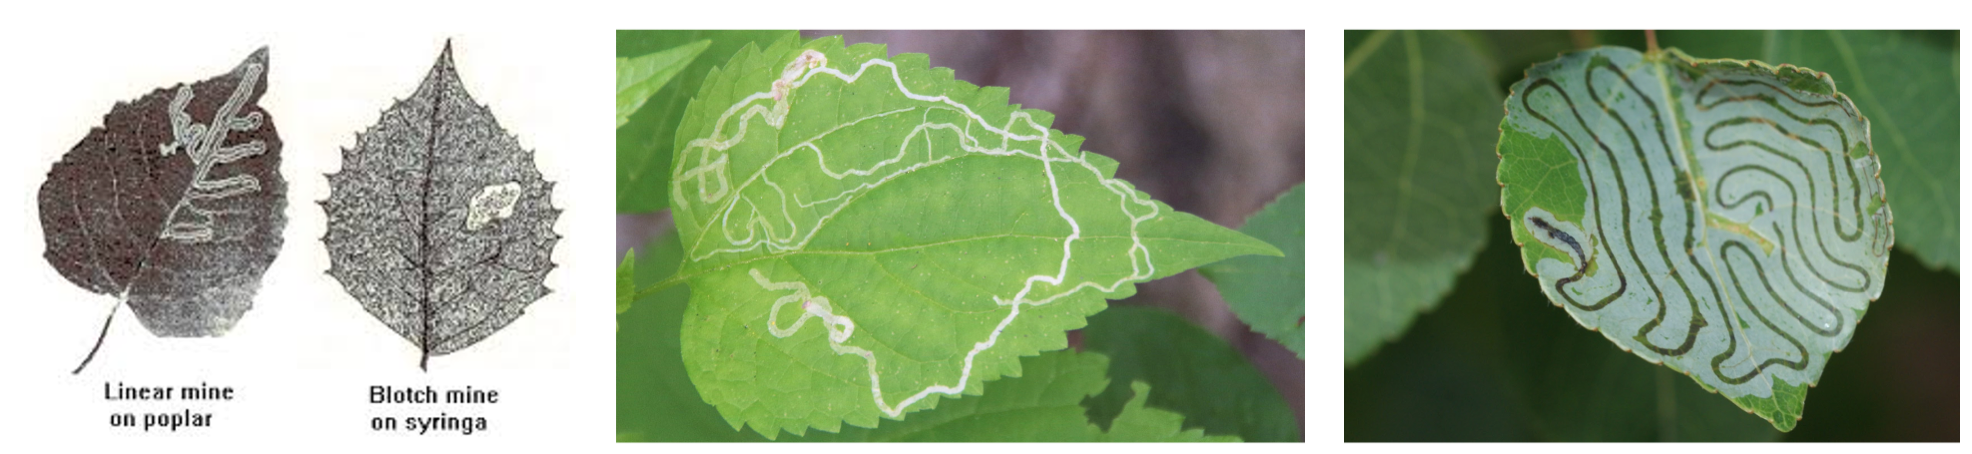
\includegraphics{protocols/images/img19.png}

}

\caption{\label{fig-mines1}Leaf mines -- Linear/Serpentine. Left/right =
single mine. Center = multiple mines}

\end{figure}%

How do you count multiple mines? It's a confusing picture but in that
way is more likely something that would be seen in the field! One of our
gall gurus (Eric LoPresti) thinks this is probably two mines. He says,
``the one that terminates at the top in a blotch and the one that
terminates at the bottom center in a wider figure 8 - looks confusing
since the bottom one doubled back, making a weird hanging trail. But you
can tell that it is a single mine, since there is no nearby really thin
trail where it starts. The intermediate width mine on the right is odd -
whether it was aborted/eaten or doubled back is not obvious to me,
however, I suspect it is the latter, as I only see two really thin
sections, both on the upper half, which indicates a start and a very
small caterpillar.''

This can get confusing, but do your best. Each count doesn't have to be
exactly right; we should still be able to get a representative count of
the distribution of damage \& mine frequencies. If in doubt with these
serpentine mines, standardize by counting only the blotchy/expanded mine
ends; this will ignore (but in a consistent way) aborted or re-started
mines. Make a note of this in the data if you choose this method.

\subsection{Leaf Mines -- Blotch Mines}\label{leaf-mines-blotch-mines}

\begin{figure}

\centering{

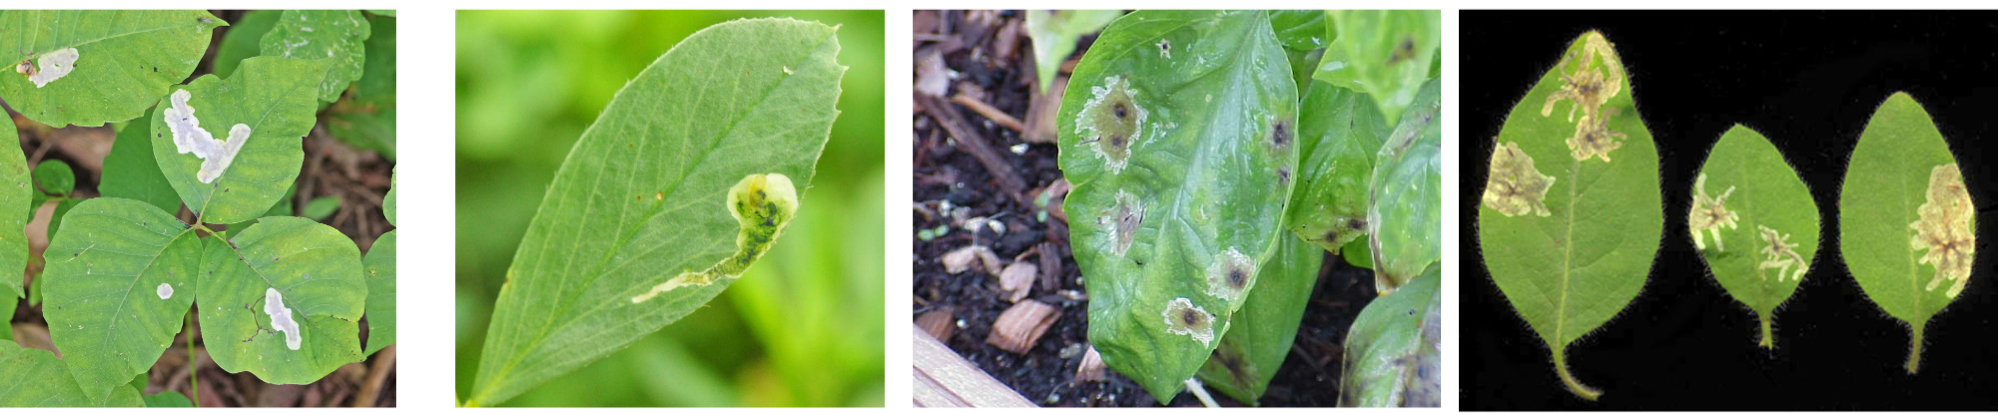
\includegraphics{protocols/images/img20.png}

}

\caption{\label{fig-mines2}Several examples of multiple blotch mines on
single leaves}

\end{figure}%

\subsection{Galls -- Leaf Galls}\label{galls-leaf-galls}

\begin{figure}

\centering{

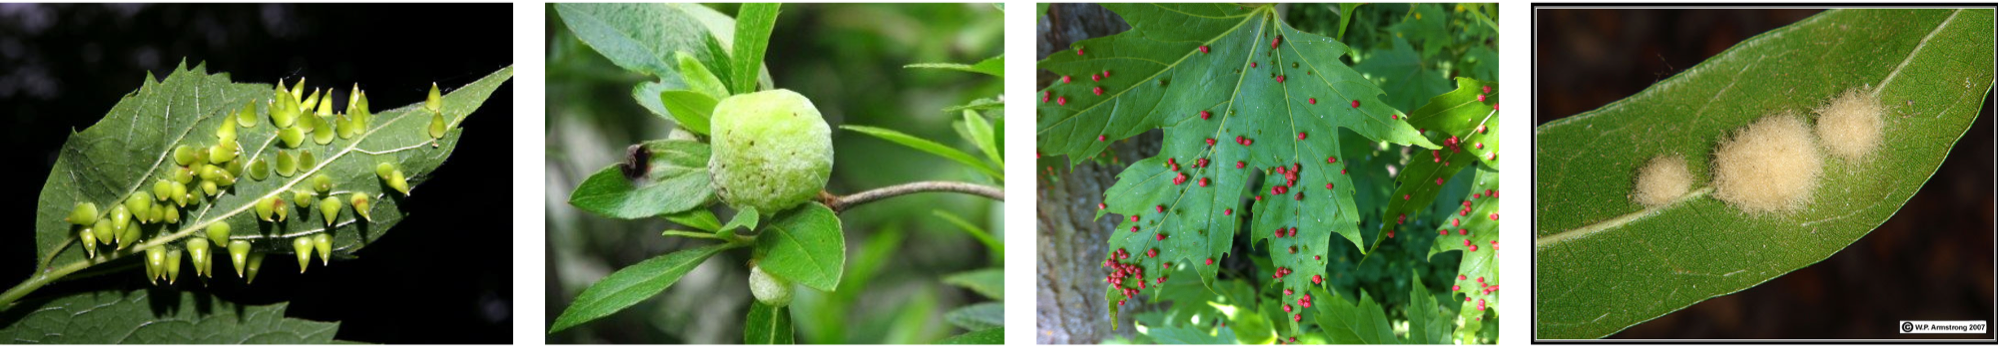
\includegraphics{protocols/images/img21.png}

}

\caption{\label{fig-galls1}Leaf Galls}

\end{figure}%

\subsection{Galls -- Stem/Branch Galls}\label{galls-stembranch-galls}

\begin{figure}

\centering{

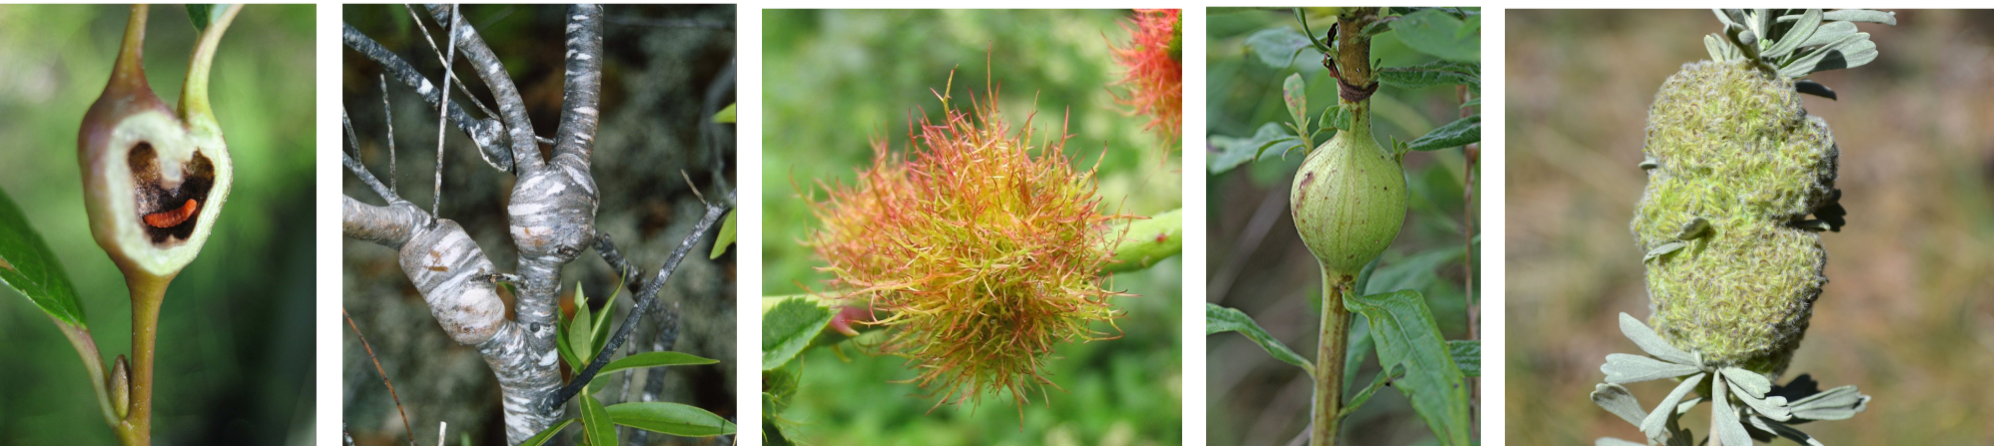
\includegraphics{protocols/images/img22.png}

}

\caption{\label{fig-galls2}Stem/Branch Galls}

\end{figure}%

\section{Insect Herbivore ID Visual
Guide}\label{insect-herbivore-id-visual-guide}

Some groups of insects (e.g.~Hemipterans, Coleopterans) include
predatory, herbivorous, and omnivorous species - and it can be
challenging to tell the two groups apart. Other groups are more certain
to be herbivores. Use this visual guide to identify insects within the
five core groups.

\subsection{Grasshoppers / crickets / katydids
(Orthoptera)}\label{grasshoppers-crickets-katydids-orthoptera}

\begin{figure}

\centering{

\captionsetup{labelsep=none}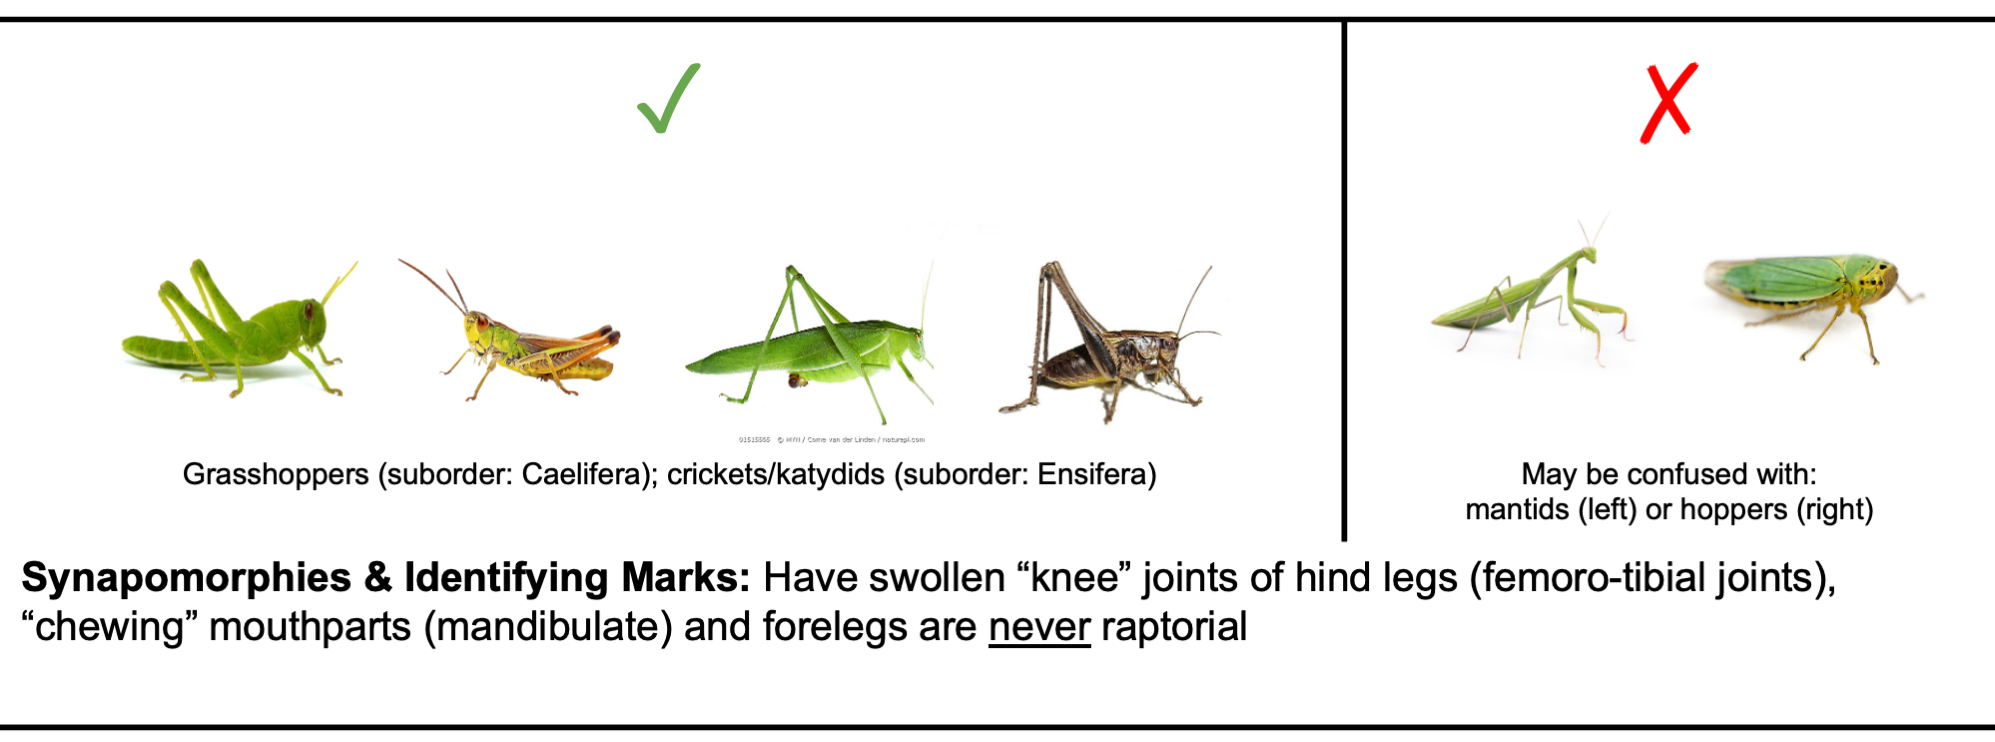
\includegraphics{protocols/images/img23.png}

}

\caption{\label{fig-herbvivores1}}

\end{figure}%

\subsection{Caterpillar-like (larval forms
ONLY)}\label{caterpillar-like-larval-forms-only}

\begin{figure}

\centering{

\captionsetup{labelsep=none}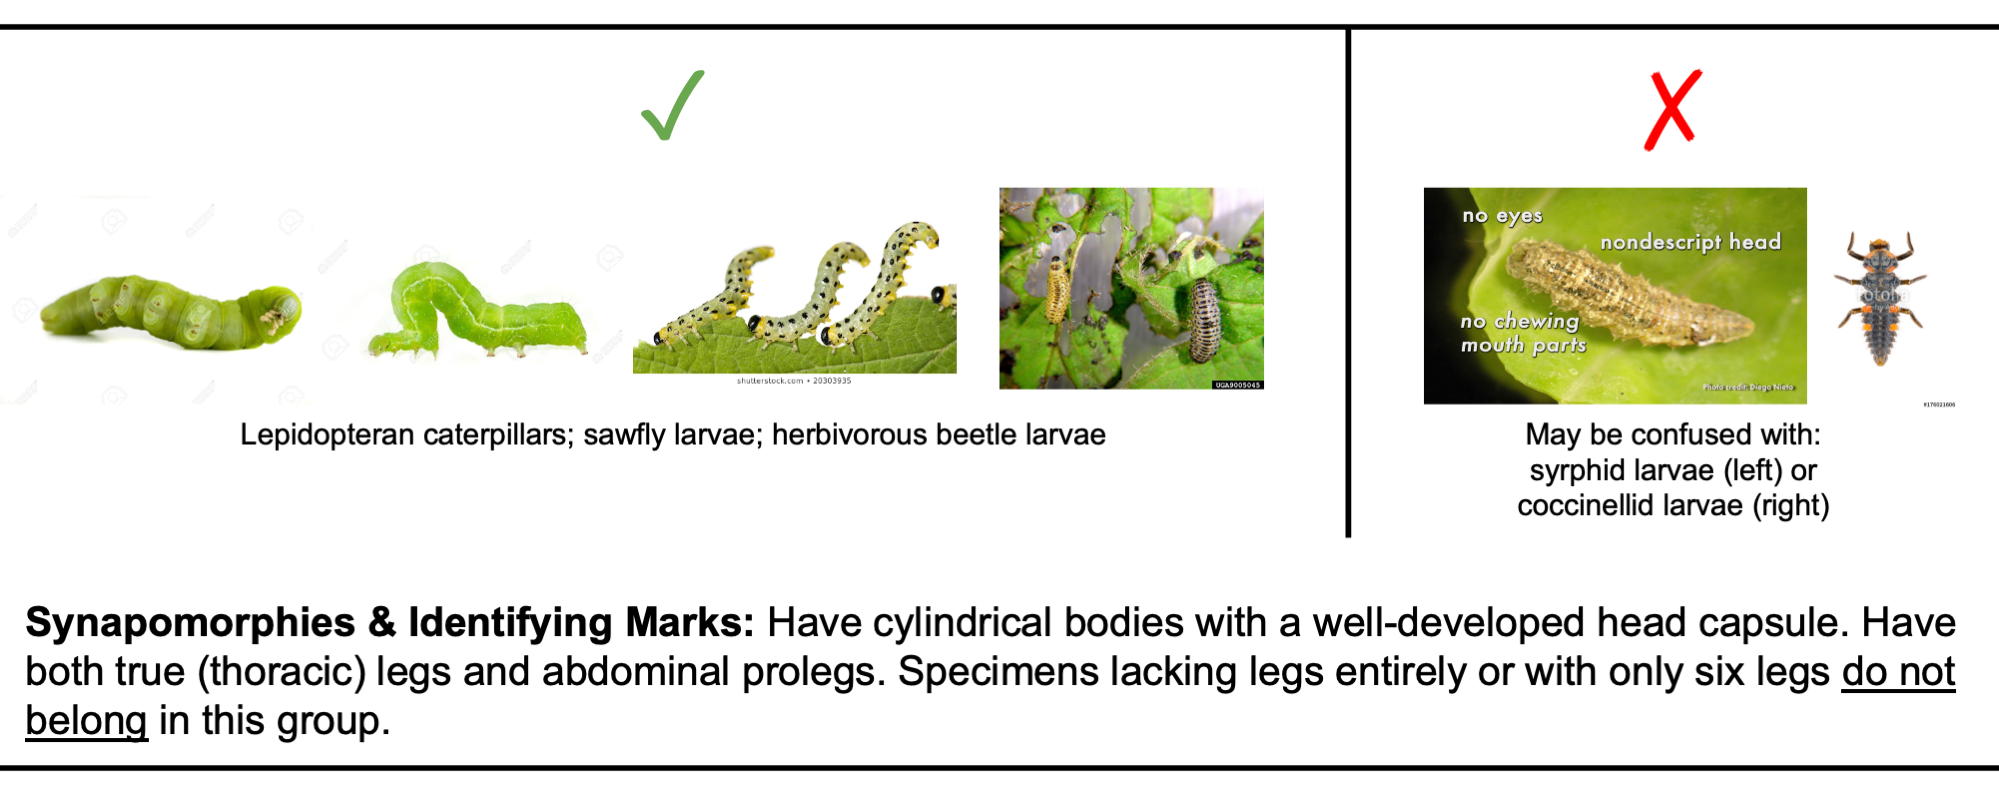
\includegraphics{protocols/images/img24.png}

}

\caption{\label{fig-herbvivores2}}

\end{figure}%

\subsection{Hoppers (Hemiptera:
Auchenorrhyncha)}\label{hoppers-hemiptera-auchenorrhyncha}

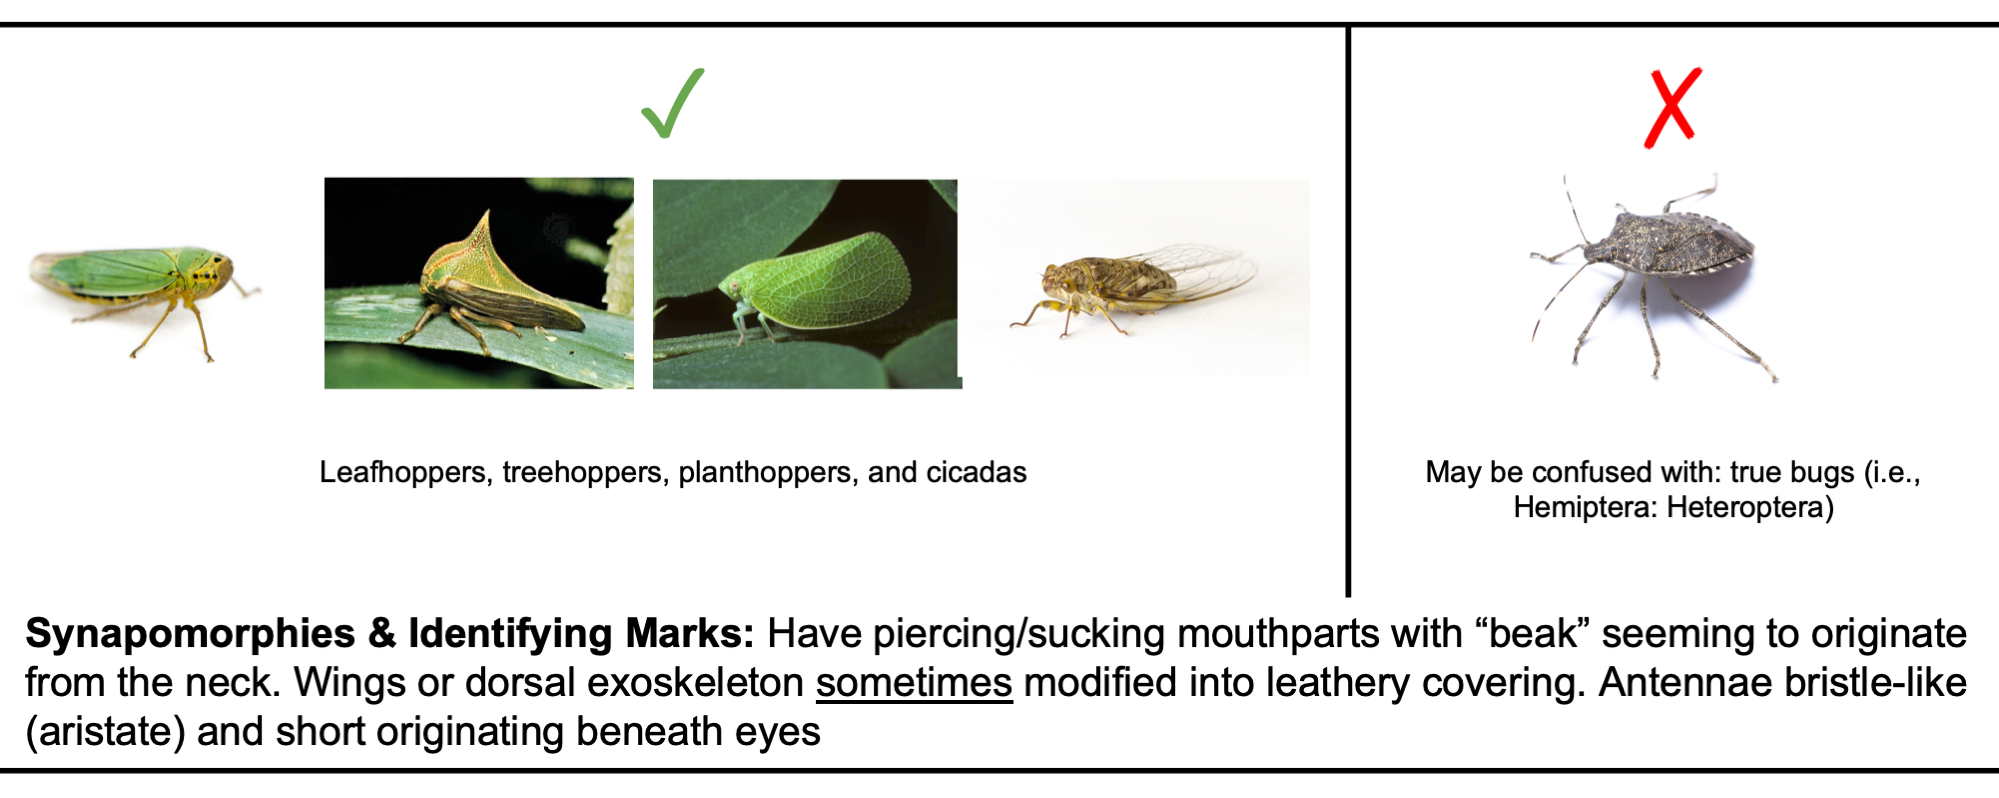
\includegraphics{protocols/images/img25.png}

\subsection{Aphids (Hemiptera:
Aphididae)}\label{aphids-hemiptera-aphididae}

\begin{figure}

\centering{

\captionsetup{labelsep=none}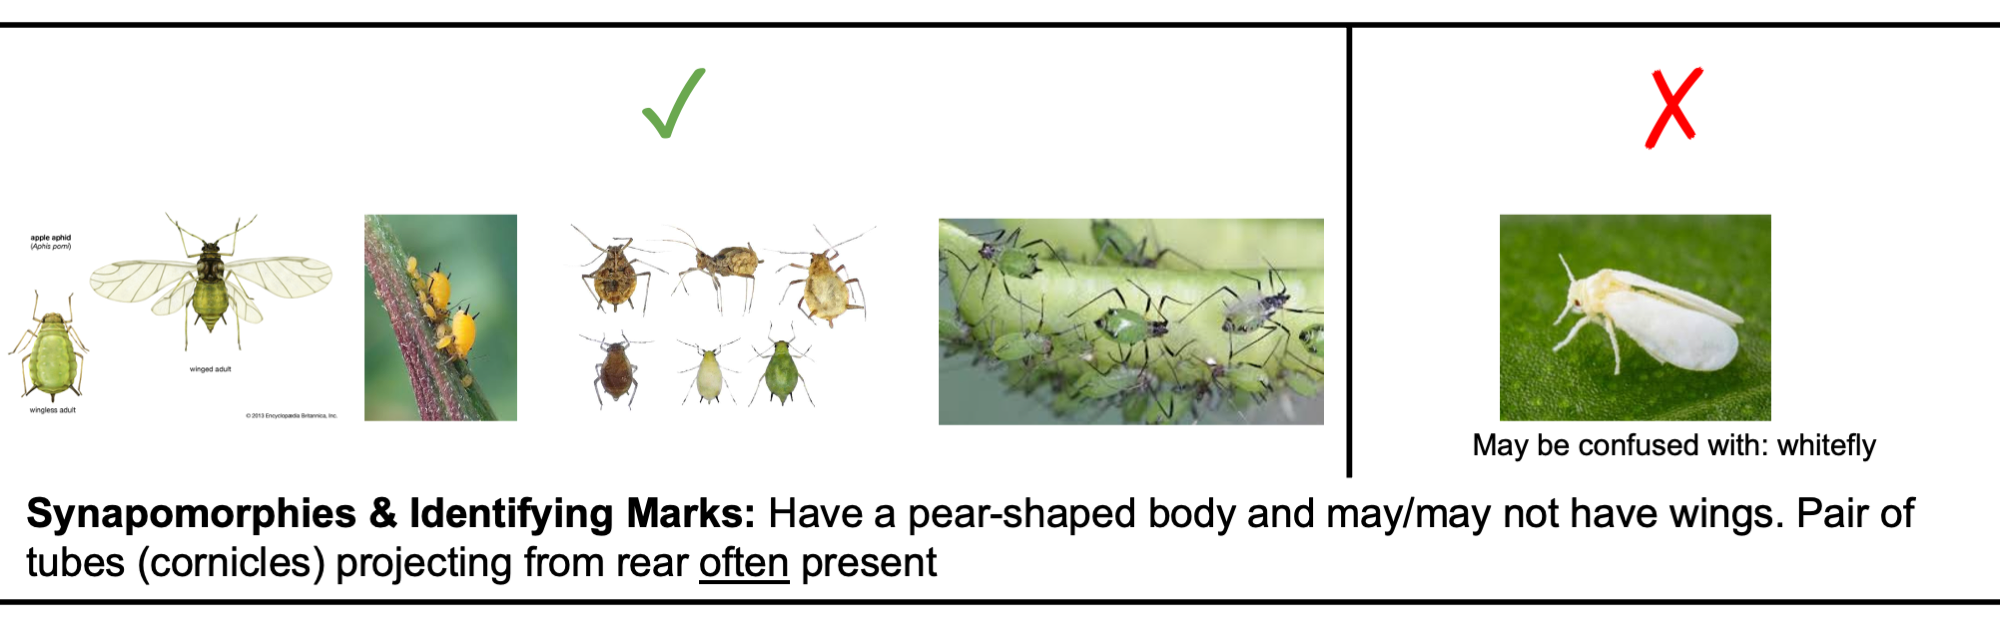
\includegraphics{protocols/images/img26.png}

}

\caption{\label{fig-herbvivores4}}

\end{figure}%

\subsection{Non-Aphid Sternorrhynchans (whiteflies, mealybugs, scale
insects)}\label{non-aphid-sternorrhynchans-whiteflies-mealybugs-scale-insects}

\begin{figure}

\centering{

\captionsetup{labelsep=none}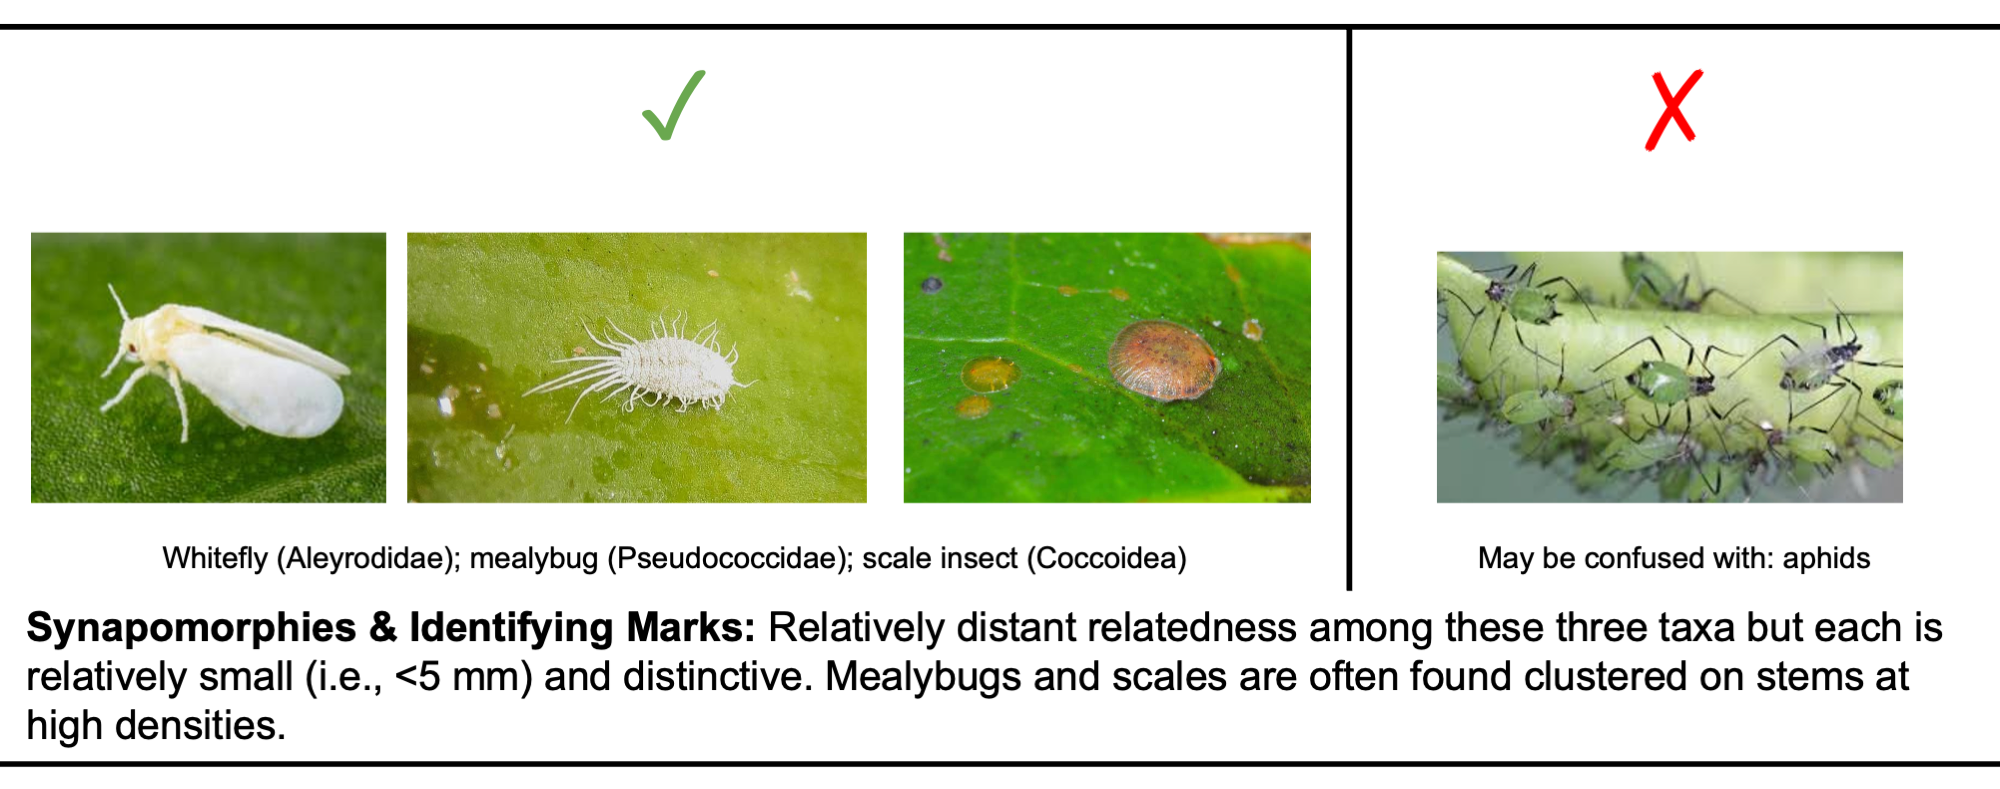
\includegraphics{protocols/images/img27.png}

}

\caption{\label{fig-herbvivores5}}

\end{figure}%

\part{Admin Tasks}

\chapter{Potential Collaborators}\label{potential-collaborators}

Potential collaborators typically get email either Will or the HerbVar
Admin gmail address. If they contact will, he replies thanking them for
their interest and forwards the email to you for follow-up.
\textbf{These are the steps for handling new expressions of interest in
collaborating:}

\begin{enumerate}
\def\labelenumi{\arabic{enumi}.}
\item
  Reply with the first email template (of 2) for prospective new
  members. Be sure to cc Will.
\item
  They respond and say:
\end{enumerate}

\begin{enumerate}
\def\labelenumi{\alph{enumi})}
\tightlist
\item
  they're not interested/have issues with the expectations.
\end{enumerate}

\begin{itemize}
\tightlist
\item
  Send them over to Will and stay on top of the email chain between them
  so you can know how he handled it. \emph{This hasn't happened, but in
  theory it could.}
\end{itemize}

\begin{enumerate}
\def\labelenumi{\alph{enumi})}
\setcounter{enumi}{1}
\tightlist
\item
  They say that sounds fine and they're still interested:
\end{enumerate}

\begin{enumerate}
\def\labelenumi{\roman{enumi}.}
\item
  Add them to the Collaborator Contact Information file
\item
  Add them as a ``Contributor'' to the HerbVar Shared Drive
\item
  Respond with the second email template (of 2)
\end{enumerate}

It is important you send the email after doing the steps i and ii
because the email template includes links that assumes (1) you have
entered preliminary information into the collaborator contact info file
and (2) they have access to everything in the HerbVar Shared Drive.

Note also that the second email template contains an onboarding document
that you may need to update going forward as onboarding needs evolve.

\chapter{Editing the Website}\label{editing-the-website}

\section{Github Access}\label{github-access}

The \href{https://herbvar.org/index.html}{HerbVar website} has been
created in R. Ask to be added as a collaborator on
\href{https://github.com/HerbVar-Network/HerbVar-website}{this
repository}.

Fork the
\href{https://github.com/HerbVar-Network/HerbVar-website}{website's
repository} to your computer. Nick Lyon initially forked the repository
so that pushes would be preserved as ``pull requests'' and could be
reviewed by Will before actually changing the website on the internet,
but this may be unnecessary depending on your comfort with this type of
coding.

\section{Making Edits}\label{making-edits}

Make whatever changes are asked for or required.

Each page of the website is saved as a separate .Rmd file and file names
mostly correspond to website tab names so it should be relatively easy
to identify which script(s) needs to be changed and implement those
edits.

The existing scripts also include plenty of examples of heading
formatting, font changes, and hyperlinks so use the existing pages to
teach yourself how to do things you don't already know how to do.

\section{Rebuilding the Website}\label{rebuilding-the-website}

Once you've made the edits, go to the ``Build'' tab on R Studio and
click ``Build Website''. This will take several minutes to process
(there will be a running list of code as it processes through each .Rmd
file) so feel free to grab a cup of coffee as this processes.

Once it completes, it will create a new tab and will pop up the new
website in your browser \textbf{but you are not yet done}!

Once that is done, in the Git tab of R Studio, select all modified files
(not just the scripts!) and commit/push them all.

Building the website may affect a lot of files in the ``libs'' folder
deep in your system (you can tell how savvy I am about this, huh?) and
these changes must also be included in the push for the website to
successfully update.

Once you've pushed these changes (and if you're working in a fork, Will
has accepted your pull request) the website on the internet should
update within 10-15 minutes so double check your work after roughly that
amount of time has passed.

\chapter{The Data Portal}\label{the-data-portal}

The data portal (link) is the preferred method for data submission for
(at least phase 2). It is written in R Shiny and is built for the phase
2 template Excel file but will work (with some warnings) for the phase 1
Excel template. This is what you need to know to change and/or
troubleshoot the app.

\section{Your Job After Someone Submits Data via the
Portal}\label{your-job-after-someone-submits-data-via-the-portal}

The data portal puts submitted data in the ``App Uploads - Phase 2''
folder (link). The portal would be self-sufficient but I have added a
step to require human involvement that I'll describe here.

\begin{enumerate}
\def\labelenumi{\arabic{enumi}.}
\item
  You need to move all files from that folder to the ``Phase II Raw
  Data'' folder (link)
\item
  All phase 2 wrangling scripts will download raw data from that latter
  folder

  \begin{enumerate}
  \def\labelenumii{\alph{enumii}.}
  \tightlist
  \item
    I've set up all of the wrangling scripts to download raw data in an
    \texttt{if()\ else\{\}} framework that will print a message
    reminding you to move the data out of the app upload folder if you
    ever forget to/don't see that new data have been uploaded
  \end{enumerate}
\item
  That's it! The data wrangling scripts will work without issue now that
  you've moved the files to the correct folder
\end{enumerate}

\section{Updating the Portal}\label{updating-the-portal}

It may become necessary to edit the portal, especially if a user emails
you indicating they had a problem and it seems like that problem is
inside of the app rather than (not to be mean) user error.

\begin{enumerate}
\def\labelenumi{\arabic{enumi}.}
\item
  All of the portal code is in the ``Data-Portal'' GitHub repository
  (link)

  \begin{enumerate}
  \def\labelenumii{\alph{enumii}.}
  \item
    The script from which the portal is created is called ``app. R'' and
    is the only file in the folder ``Data Portal Actual''
  \item
    You will also need the ``deployment-faq. R'' script in the ``Support
    Scripts'' folder in order to deploy the app after you have
    made/tested any changes to the portal's code. i. If it is of
    interest, the ``Support Scripts'' folder also includes my (Nick's)
    incremental forays into the world of Shiny so you can see the first
    through eighth versions of the portal before getting to a version
    that was deployed.
  \end{enumerate}
\item
  Before changing the portal I strongly recommend asking the user who
  pointed out the issue for a screenshot of how they've filled the app
  out immediately before the error

  \begin{enumerate}
  \def\labelenumii{\alph{enumii}.}
  \item
    The error is almost always (or at least has usually been) something
    to do with how the user filled out the app or attached their data.
    If that is the case, you may need only point that out to them (in a
    polite way) and go about your day
  \item
    Also, the only time the app can break is when they click the
    ``Submit Data'' button. Prior to that, the app is not actually
    trying to do anything, so any app-breaking user error will not be
    apparent to them until they click that button
  \item
    HOWEVER, some users who experience an issue actually create a larger
    error that will prevent them from uploading their data even after
    you point the app key issue out to them. To handle such cases, see
    the next subsection. The importance of this is also noted in part d
    of the next bullet 3. To change the data portal do the following:
  \end{enumerate}

  \begin{enumerate}
  \def\labelenumii{\arabic{enumii}.}
  \tightlist
  \item
    First, modify the app. R script as desired. Note that every Shiny
    App consists of three components: (1) the user interface, (2) the
    server that includes all the internal mechanisms for the portal, and
    (3) a ShinyApp() call that combines the UI and server.
  \end{enumerate}

  \begin{enumerate}
  \def\labelenumii{\roman{enumii}.}
  \item
    If the app is not working, it will likely be in the server component
  \item
    If the app doesn't look right but does function appropriately,
    modify the UI
  \item
    If the app does not collect some information that it should, you
    will need to change both the UI and server
  \item
    The ShinyApp call at the end never needs to be modified so don't
    worry about that bit
  \end{enumerate}

  \begin{enumerate}
  \def\labelenumii{\arabic{enumii}.}
  \setcounter{enumii}{1}
  \tightlist
  \item
    Second, test the app on your computer by running the app
  \end{enumerate}

  \begin{enumerate}
  \def\labelenumii{\roman{enumii}.}
  \item
    In R Studio, the top right of the R script panel containing a
    ShinyApp has a ``Run App'' button to the right of a green `play'
    button
  \item
    Pushing this button will create a local version of the portal that
    functions as the app will but does not deploy to the internet (yet).
  \item
    I recommend submitting a test data file (see the folder of the same
    name for pre-built phase 2 data that you can use) from start to
    finish to ensure that everything works as desired.
  \end{enumerate}

  \begin{enumerate}
  \def\labelenumii{\arabic{enumii}.}
  \setcounter{enumii}{2}
  \tightlist
  \item
    Third, once you are satisfied with your changes, you can deploy the
    app to replace the old publicly-available version on the internet!
  \end{enumerate}

  \begin{enumerate}
  \def\labelenumii{\roman{enumii}.}
  \item
    In the ``deployment-faq. R'' script, you will load the ``rsconnect''
    library (line 12) and then use it to redeploy the app (line 18)
  \item
    Running the deployApp function will prompt you in the console to
    type a ``Y'' if you're sure that you want to re-deploy the app
  \item
    After you type ``Y'' and hit return in the console, it will build
    your new portal, terminate the old one, replace the old with the
    new, and then activate the new one for all users
  \item
    You'll know this is done when R automatically kicks you to a new tab
    in your web browser with the new portal open
  \end{enumerate}
\item
  Fourth, and this is crucial, if your changes to the app were because a
  user was having issues, you need to delete any files they successfully
  submitted

  \begin{enumerate}
  \def\labelenumii{\roman{enumii}.}
  \tightlist
  \item
    See the next sub-section for information on how to do this/why it
    needs to be done
  \end{enumerate}
\item
  Finally, notify the user that initially contacted you letting them
  know that you have resolved the issue on your end, thanking them for
  bringing it to your attention, and inviting them to reach out again if
  it still isn't working for them
\end{enumerate}

\section{Deleting Old Data}\label{deleting-old-data}

The data portal will fail if it tries to create two files of the same
name.

\begin{enumerate}
\def\labelenumi{\arabic{enumi}.}
\item
  The amount of information used to create the file name means that it
  is incredibly unlikely that two different users could accidentally
  create the same file name
\item
  BUT, as mentioned in the ``Updating the Portal'' section, it is
  entirely possible (and has happened previously) for the same user to
  try to submit data more than once and inadvertently create two files
  of the same name

  \begin{enumerate}
  \def\labelenumii{\alph{enumii}.}
  \item
    This occurs when the following happens:
  \item
    First, the user tries to submit data using the portal but something
    goes wrong so their data aren't actually submitted (but a blank
    GoogleSheet of the user-supplied name is created)
  \end{enumerate}

  \begin{enumerate}
  \def\labelenumii{\roman{enumii}.}
  \setcounter{enumii}{1}
  \item
    Second, the user tries to re-submit data (possibly after you fix the
    issue in the portal and notify them) but the blank document they
    unknowingly created earlier now causes a different error (i. e. ,
    that there are now two files of the same name)
  \item
    Unfortunately, because Shiny Apps are noninteractive (see the
    ``Service Account FAQ'' section) the user will never be provided
    with an informative error (neither will you) so you'll need to
    diagnose this as part of your `fixing the app' process
  \end{enumerate}
\item
  To resolve this, I (Nick) have created a second Shiny App that is not
  deployed

  \begin{enumerate}
  \def\labelenumii{\alph{enumii}.}
  \tightlist
  \item
    To be clear, it should never be deployed to prevent its accidental
    (mis)use by general HerbVar members
  \end{enumerate}
\item
  Justification and location of the second app

  \begin{enumerate}
  \def\labelenumii{\alph{enumii}.}
  \item
    The second app is in the ``Data-Portal-Maintenance'' GitHub
    repository (link)
  \item
    The ``Service Account FAQ'' section below gives more context but in
    brief: the `app key' file that the data portal makes users attach is
    actually activating a sort of Google robot with the authority to
    create Google Sheets and move them i. This is necessary because an
    online portal cannot send an authorization request to each user in
    the way that R/R Studio does when such code is run on a local
    computer (again, see the ``Service Account FAQ'' section for more
    details)
  \item
    This `robot' then is the true owner of all data files submitted
    through the app
  \item
    The portal cannot submit data to a Shared Drive (due to issues with
    the R packages that connect R and Google that are outside of our
    control) so this is an unavoidable state
  \item
    So, if a user accidentally creates a flawed data object of the same
    name as their real data they will be unable to submit their real
    data until the flawed one is deleted
  \item
    HOWEVER, because the `robot' owns those files, you cannot actually
    delete any of its files (when you ``delete'' a file you don't own
    you actually just remove yourself as a collaborator with no effect
    on the original file)
  \item
    Here is where we get to the need of a second app
  \item
    The robot's GoogleDrive cannot be accessed via a Graphical User
    Interface in the way that you would access any other Google Drive
  \end{enumerate}

  \begin{enumerate}
  \def\labelenumii{\roman{enumii}.}
  \setcounter{enumii}{1}
  \item
    So, to truly delete these files so a user can re-submit their data
    successfully, you will need to use this second app
  \item
    If you fail to delete the bad data, the user will never be able to
    successfully submit data of the same name 1. In theory, you could
    ask them to re-name their file in some slightly different way (i. e.
    , by changing their site name), but that would still have this
    flawed data floating in the ether which is not desirable
  \end{enumerate}
\item
  Tutorial of the second app

  \begin{enumerate}
  \def\labelenumii{\alph{enumii}.}
  \item
    To reiterate, this Shiny app should never be deployed.
  \item
    You will see why, but for the moment, take my word on it that
    deploying this app has a non-zero potential of permanently deleting
    data files you actually want
  \end{enumerate}

  \begin{enumerate}
  \def\labelenumii{\roman{enumii}.}
  \setcounter{enumii}{1}
  \tightlist
  \item
    By keeping the script in GitHub and locking view access to only Will
    \& the Data Scientist, we preserve its utility without opening
    Pandora's box of deploying it and possibly having an HerbVar member
    use it improperly
  \end{enumerate}

  \begin{enumerate}
  \def\labelenumii{\alph{enumii}.}
  \setcounter{enumii}{1}
  \item
    The second app is fully contained in the ``check-service-acct-files.
    R'' script (the only script in this project)
  \item
    Open that script and click the ``Run App'' button in the top right
    of the R script pane of R Studio
  \item
    As with updating the data submission portal, this will create a new
    tab in your web browser that contains a fully functional (but not
    available on the internet) version of the app
  \item
    The app is divided into three columns that you will proceed through
    from left to right
  \item
    First, download and attach the key for the service account that owns
    the files you want to look through (column 1)
  \item
    For now we only have one service account for phase
  \end{enumerate}
\item
  I recommend creating a new service account for each subsequent phase
  to evade data storage limits and partition sources of error in a
  clean, behind-the-scenes sort of way
\end{enumerate}

\begin{enumerate}
\def\labelenumi{\roman{enumi}.}
\setcounter{enumi}{1}
\tightlist
\item
  See below for information on creating Service Accounts
\end{enumerate}

\begin{enumerate}
\def\labelenumi{\alph{enumi}.}
\setcounter{enumi}{5}
\item
  Second, click the ``Authorize'' button to notify the app that it
  should attach the app key (column 1)
\item
  This may take a few seconds but should generate a full list of all
  files owned by the robot (i. e. , owned by the service account) g.
  Third, after looking at the list of files, click the ``Extract File
  Names'' button (column 2)
\item
  This just populates the third column so don't worry about the violence
  implied by the verb `extract'
\item
  Fourth, scroll through the drop down list (column 3) and select the
  file you want to delete (could be a test data file or the product of a
  specific user's failed attempt to upload their data)
\item
  Fifth, above the dropdown menu, check the ``Yes'' option beneath ``I
  am ready to delete a file''
\item
  I recommend doing this after selecting a file to further mitigate the
  risk of deleting the wrong file j. Sixth, click the ``Delete Selected
  File'' button i. Because you attached the service account key in
  column 1, you are viewing and interacting with the robot's files as
  the robot (rather than as yourself)
\end{enumerate}

\begin{enumerate}
\def\labelenumi{\roman{enumi}.}
\setcounter{enumi}{1}
\tightlist
\item
  This gives you access to actually delete files rather than just--as
  mentioned before--removing yourself from seeing the file
\end{enumerate}

\begin{enumerate}
\def\labelenumi{\alph{enumi}.}
\setcounter{enumi}{10}
\item
  Seventh, once a dialogue has popped up below the ``Delete Selected
  File'' button confirming the file has been deleted, click the ``Update
  List of Drive Contents'' button
\item
  This will update the dropdown menu with the new file list now that the
  file you marked for deletion has been erased l. Finally, scroll
  through the dropdown menu (or look at the list of files in column 2)
  to ensure that all problem files have been deleted 6. After you've
  gone through that process to delete the flawed file, you can notify
  the user that it is safe for them to resubmit their data
\item
  This is all likely too much information for the user though so I
  suggest that you just tell them you have fixed the data portal and
  leave it at that
\end{enumerate}

\begin{enumerate}
\def\labelenumi{\arabic{enumi}.}
\setcounter{enumi}{6}
\tightlist
\item
  Also, I have written the app to work with any service account key that
  owns Google files so unless the structure of future phases' data
  portals changes massively, this app should be sufficient for all
  issues involving service account-owned files in the future
\end{enumerate}

\section{Service Account FAQ Background
Information}\label{service-account-faq-background-information}

The data submission portal accepts uploaded data locally and then (1)
creates a Google Sheet version of the data and (2) moves that sheet into
the designated folder in the HerbVar Admin Drive. However, the Shiny app
is ``non-interactive'' (see gargle's vignette) which means that a user
cannot input a gmail or access token to tell Google Drive/Sheets who is
creating/moving files. A ``service account'' is necessary to get around
this.

A service account is essentially a robot that we pre-approve to (1)
create google sheets, (2) move files, and (3) have access to the
folder(s) we want those sheets made in/moved to. ○ Side note: see the
list of people with access to the folder the Shiny portal saves files to
and you'll see the service account I created in that list.

To create/manage a service account you need to use ``Google Cloud
Platform'' as described below:

\section{Tutorial}\label{tutorial}

\begin{enumerate}
\def\labelenumi{\arabic{enumi}.}
\item
  Sign into the herbvar@gmail. com Google Account
\item
  Visit the Google Cloud Platform (link)

  \begin{enumerate}
  \def\labelenumii{\alph{enumii}.}
  \item
    If there is a pale red/pink error saying you don't have sufficient
    permissions to view the page, select the herbvar@gmail. com account
    from the drop down in the top right of the screen
  \item
    The page should then re-load to the dashboard
  \end{enumerate}
\item
  Don't get overwhelmed by the level of detail on this page!
\item
  In the left sidebar, click ``APIs \& Services'' and within that menu
  click ``Credentials''
\item
  Click the service account name in the ``Service Accounts'' list at the
  bottom of the screen
\item
  Keys can be managed in the ``Keys'' tab
\item
  In the event of a security breach (not sure what that would look like
  but still good to have the contingency), delete the existing keys and
  create a new one
\item
  Download that key and replace the one HerbVar members have access to
  with the new key file.
\item
  If creating a new key or service account prompts you to add
  permissions to the account be sure that it includes BOTH the
  GoogleSheets API AND the GoogleDrive API

  \begin{enumerate}
  \def\labelenumii{\alph{enumii}.}
  \tightlist
  \item
    Both are needed because the data portal uses the service account key
    to both create a GoogleSheet (using the eponymous API) and move that
    GoogleSheet (using the GoogleDrive API)
  \end{enumerate}
\end{enumerate}

\chapter{Google Drive Structure}\label{google-drive-structure}

This project has a lot of files coming and going so this is a brief
description of all of those folders.

\section{Phase I Data Wrangling}\label{phase-i-data-wrangling}

\begin{itemize}
\item
  HerbVar Phase I Data
\item
  All Uploads
\item
  All of the phase 1 raw data (and we've since moved to phase 2 so there
  should not be any more new data)
\item
  Phase I
\item
  Herbivore Data
\item
  herbivoreData (from the eponymous Excel sheet) raw, tidied at
  plant-level (one row per plant) and tidied at survey level (one row
  per survey)
\item
  Raw is the herbivore columns sliced off of the plantData sheet as part
  of the main wrangling script
\item
  Phase I - Primary Productivity
\item
  Primary productivity metadata to go along with phase 1 data
\item
  Phase I - Reproductive Data
\item
  Raw reproductive data columns sliced off of the plantData sheet as
  part of the main wrangling script
\item
  Phase I - Richness Data
\item
  Extracted native/invasive species richness from Ellis et al.~2012
\item
  Phase I - siteData - Tidied version of siteData (from eponymous Excel
  sheet)
\item
  Phase I - Survey Indices - Attempt (later abandoned) to split off just
  the site and plant-identifying information without any of the
  ``actual'' data. This would allow wide sharing of location information
  to enable all interested HerbVar members to harvest publicly-available
  metadata
\item
  Phase I Data - Wrangled
\item
  The ``abiotic'' (i.e., climatic) data for each site's lat/long
  coordinates
\item
  The tidied plant-level data (one row per plant) for all phase 1 data
\item
  The tidied survey-level data (one row per survey) for all phase 1 data
\item
  HerbVar Foliage Index.xlsx - Index describing whether each species
  (from each PI) is deciduous, evergreen, or annual (this information
  was integrated into the phase 2 data submission portal so no
  equivalent Google Sheet will exist for phase 2
\end{itemize}

\section{Phase II Data Wrangling}\label{phase-ii-data-wrangling}

\begin{itemize}
\item
  \_Data Submitted Via Email - I need to put it through the App - This
  is a clearinghouse for all raw phase 2 data that users send via email
  rather than using the submission portal. While discouraged, we don't
  want to completely block data in such instances. So, once you receive
  data via email, drop it into this folder until you have the time to
  run it through the app (the handful of times this has occurred the
  data went through the portal fine, users just got frustrated from
  unrelated things)
\item
  App Uploads - Phase 2 - Raw data submitted via the portal arrive here
\end{itemize}

\section{Phase II Completed Surveys
Versions}\label{phase-ii-completed-surveys-versions}

\begin{itemize}
\tightlist
\item
  All phase 2 wrangling scripts copy the completed surveys file with a
  time stamp to this folder for posterity. I can think of no direct
  utility of these backups but it doesn't hurt to save them -
\end{itemize}

\section{Phase II Metadata}\label{phase-ii-metadata}

\begin{itemize}
\tightlist
\item
  Rather than have separate folders for each metadata type (as was the
  case in phase 1) I have created this folder to contain them. Only
  abiotic (i.e., climatic) data have been retrieved so far but all
  should be placed here to keep the Drive folder hierarchy clean
\end{itemize}

\section{Phase II Raw Data}\label{phase-ii-raw-data}

\begin{itemize}
\tightlist
\item
  All data submitted through the submission portal should be manually
  moved from the ``App Uploads - Phase 2'' folder to here. The wrangling
  scripts will prompt you to do this if you do not before running them.
\end{itemize}

\section{Phase II Wrangled Data -
\ldots{}}\label{phase-ii-wrangled-data--}

\begin{itemize}
\tightlist
\item
  Each sheet of the Excel file has its own version of the above folder
  where the ellipses (\ldots) is replaced by that sheet's name. Where
  applicable (e.g., plantData, reproData, herbivoreData) there are
  survey-level (i.e., one row per survey) versions of the data
\end{itemize}

\section{Miscellaneous Other Files}\label{miscellaneous-other-files}

\emph{Note: this heading is not a folder name but refers to the random
other files in the Drive.}

\begin{itemize}
\tightlist
\item
  This manual is unfiled in the Drive!
\item
  The Data Management Plan (DMP) in graphical form
\item
  Tutorials for one-off tasks you may need to explain to others
\end{itemize}

\chapter{Wrangling Repository}\label{wrangling-repository}

The \href{https://github.com/HerbVar-Network/Wrangling}{Wrangling
Repository} contains scripts for data wrangling for all phases of the
project. It takes in raw data and outputs analysis/visualization-ready
.csv files.

It will be the primary home for this Research/Admin Position (or at
least it was for me) so it may help to give you a brief explanation of
each of the main scripts. Here's the link.

\section{Misc. Non-Manuscript Subset
Scripts}\label{misc.-non-manuscript-subset-scripts}

So far, this only includes the script to separate out PlantPopNet
members' data to make sharing that with PPN leadership (upon request)
simpler

\section{Phase 1 Scripts}\label{phase-1-scripts}

\texttt{phase\ 1\ abiotic\ wrangling.R}: Wrangles WORLDCLIM climatic
data for phase 1 surveys.

\texttt{phase\ 1\ herbivoreData\ wrangling.R}: Wrangles any information
to do with herbivores from phase 1.

\texttt{phase\ 1\ plant\ richness\ wrangling.R}: Extracts interpolated
native/invasive species richness information from Ellis et al.~2012
shapefiles.

\texttt{phase\ 1\ primary\ productivity.R}: Extracts primary
productivity data from satellite data for phase 1 surveys.

\texttt{phase\ 1\ shareable\ index.R}: Creates files of only location
information for phase 1 sites to enable other HerbVar collaborators to
harvest metadata without sharing ``actual'' data.

\texttt{phase\ 1\ siteData\ wrangling.R}: Wrangles information from
siteData sheet of template Excel file.

\texttt{phase\ 1\ soil\ data\ wrangling.R}: Placeholder describing where
soil data may someday be acquired. For now, the relevant R package does
not work (though their team is aware of and working on this issue).

\texttt{phase\ 1\ survey-lvl\ summarizing.R}: Summarizes the tidy
plant-level (one row per plant) phase 1 data to survey-level (one row
per survey).

\texttt{phase\ 1\ wrangling.R}: Takes all the separate phase 1 raw data
files combines and wrangles them to plant-level (one row per plant).

\section{Phase 2 Scripts}\label{phase-2-scripts}

\texttt{phase\ 2\ densityData\ wrangling.R}: Wrangles eponymous sheet
from template Excel file.

\texttt{phase\ 2\ herbivoreData\ wrangling.R}: Wrangles eponymous sheet
from template Excel file (at both plant-level and survey-level).

\texttt{phase\ 2\ metadata}abiotic.R`: Extracts WORLDCLIM climatic data
from phase 2 site locations (requires tidy file from siteData wrangling
script).

\texttt{phase\ 2\ newColumns\ wrangling.R}: Wrangles eponymous sheet
from template Excel file.

\texttt{phase\ 2\ notes\ wrangling.R}: Wrangles eponymous sheet from
template Excel file.
\texttt{phase\ 2\ plantData\ survey-lvl\ summarizing.R}: Summarizes tidy
plantData to survey-level (i.e., one row per survey).

\texttt{phase\ 2\ plantData\ wrangling.R}: Wrangles eponymous sheet from
template Excel file (at ONLY plant-level).

\texttt{phase\ 2\ reproData\ wrangling.R}: Wrangles eponymous sheet from
template Excel file at plant-level only (survey level absent because
insufficient raw data at this point).

\texttt{phase\ 2\ siteData\ wrangling.R}: Wrangles eponymous sheet from
template Excel file.

\section{Script Archive}\label{script-archive}

All ``actual'' scripts (i.e., those used in day-to-day wrangling) should
have a consistent aesthetic and comment structure (as well as being
primarily tidyverse-based). When others contribute code, duplicate the
file and edit one version to match internal standards. The second
version goes here to be preserved in its original form as a back-up

\section{Singleton Tasks}\label{singleton-tasks}

Any scripts written to accomplish a `one-off' task I thought unlikely to
be repeated regularly are placed here. Some of them may include
operations that could be useful in other contexts tough!

\section{Manuscript Subsetting
Scripts}\label{manuscript-subsetting-scripts}

Each script is dedicated for a single HerbVar manuscript and does the
subsetting and/or column selection necessary to create a tidy data file
of only what authors request to test their hypotheses

\chapter{To-Do List for Manual}\label{to-do-list-for-manual}

(as of 2/1/22)

\begin{enumerate}
\def\labelenumi{\arabic{enumi}.}
\tightlist
\item
  Edit the ``Google Drive'' chapter
\item
  Convert ``data portal troubleshooting'' to a flowchart/checklist
\item
  Edit Protocols:
\end{enumerate}

\begin{enumerate}
\def\labelenumi{\alph{enumi}.}
\tightlist
\item
  Insert Photos
\item
  link to pdf versions for downloading by users
\item
  edit / correct formatting
\end{enumerate}

\begin{enumerate}
\def\labelenumi{\arabic{enumi}.}
\setcounter{enumi}{3}
\tightlist
\item
  review and expand the workflow chapter
\item
  review and expand the data analysis chapter; include tutoriual for
  repo
\item
  review and expand the publications chapter; include tutoriual for repo
\item
  References/multiple .bib files
\item
  herbvar publications, herbvar presentations
\item
  add tutorial for editing the manual and publishing with actions
  https://quarto.org/docs/publishing/github-pages.html
\end{enumerate}

\begin{center}\rule{0.5\linewidth}{0.5pt}\end{center}

Unfortunately I (Nick) took a new position while there were still some
loose ends left hanging but I can list them here so they don't
completely fall between the cracks -

\section{Data Use Agreement}\label{data-use-agreement}

I wrote a data use contract for HerbVar members to sign upon joining the
Network so that we can have them release rights to their data to us (and
promise not to share the larger datafiles produced by the collaboration
- The email conversation for getting the Planning Group's feedback and
green light has the subject line ``HerbVar Data Sharing Agreement
Draft'' - The relevant Google Drive folder is linked here and lives in
the ``HerbVar Management'' Shared Drive -

\section{Authorship Guidelines
Conversation}\label{authorship-guidelines-conversation}

The Planning Group was in the midst of deciding on revised authorship
guidelines to catch some edge cases that fell outside of the earlier
authorship policy. - You can catch up on this in the email thread with
the subject ``HerbVar Authorship Criteria Questions''

\section{Herbivore Protocol Gray
Area}\label{herbivore-protocol-gray-area}

The Herbivore protocol is written to prioritize taxonomic identification
of insects. However, many researchers are also (and sometimes more)
interested in functional identification of insects. Our current approach
to the template Excel file allows people to add their own columns as
they see fit but this makes later switching from functional to taxonomic
(or vice versa) difficult. So, there is a draft email in the
herbvar@gmail account to send when a panel of herbivore experts has been
assembled to resolve this uncertainty

\bookmarksetup{startatroot}

\chapter*{References}\label{references}
\addcontentsline{toc}{chapter}{References}

\markboth{References}{References}

A .bib file of all HerbVar publications is available for download here.

\phantomsection\label{refs}
\begin{CSLReferences}{1}{0}
\bibitem[\citeproctext]{ref-bolandTenSimpleRules2017}
Boland, M. R., K. J. Karczewski, and N. P. Tatonetti. 2017.
\href{https://doi.org/10.1371/journal.pcbi.1005278}{Ten {Simple Rules}
to {Enable Multi-site Collaborations} through {Data Sharing}}. PLOS
Computational Biology 13:e1005278.

\bibitem[\citeproctext]{ref-bragaNotJustProgrammers2023}
Braga, P. H. P., K. Hébert, E. J. Hudgins, E. R. Scott, B. P. M.
Edwards, L. L. Sánchez Reyes, M. J. Grainger, V. Foroughirad, F.
Hillemann, A. D. Binley, C. B. Brookson, K. M. Gaynor, S. Shafiei Sabet,
A. Güncan, H. Weierbach, D. G. E. Gomes, and R. Crystal-Ornelas. 2023.
\href{https://doi.org/10.1111/2041-210X.14108}{Not just for programmers:
{How GitHub} can accelerate collaborative and reproducible research in
ecology and evolution}. Methods in Ecology and Evolution 14:1364--1380.

\bibitem[\citeproctext]{ref-brunaGithubToolPromoting2024}
Bruna, E. M. 2024, March. Github as a tool for promoting reproducibility
and collaboration in the {HerbVar Network}. HerbVar Steeting Committee
Meeting.

\bibitem[\citeproctext]{ref-champieuxTenSimpleRules2023}
Champieux, R., A. Solomonides, M. Conte, S. Rojevsky, J. Phuong, D. A.
Dorr, E. Zampino, A. Wilcox, M. B. Carson, and K. Holmes. 2023.
\href{https://doi.org/10.1371/journal.pcbi.1011136}{Ten simple rules for
organizations to support research data sharing}. PLOS Computational
Biology 19:e1011136.

\bibitem[\citeproctext]{ref-goodmanTenSimpleRules2014}
Goodman, A., A. Pepe, A. W. Blocker, C. L. Borgman, K. Cranmer, M.
Crosas, R. D. Stefano, Y. Gil, P. Groth, M. Hedstrom, D. W. Hogg, V.
Kashyap, A. Mahabal, A. Siemiginowska, and A. Slavkovic. 2014.
\href{https://doi.org/10.1371/journal.pcbi.1003542}{Ten {Simple Rules}
for the {Care} and {Feeding} of {Scientific Data}}. PLOS Computational
Biology 10:e1003542.

\bibitem[\citeproctext]{ref-harperPopulationBiologyPlants1977}
Harper, J. L. 1977. Population biology of plants. Academic Press.

\bibitem[\citeproctext]{ref-herbenEvolutionClonalGrowth2020}
Herben, T., and J. Klimešová. 2020.
\href{https://doi.org/10.1111/nph.16188}{Evolution of clonal growth
forms in angiosperms}. New Phytologist 225:999--1010.

\bibitem[\citeproctext]{ref-kimImplementingGitHubActions2022}
Kim, A. Y., V. Herrmann, R. Barreto, B. Calkins, E. Gonzalez-Akre, D. J.
Johnson, J. A. Jordan, L. Magee, I. R. McGregor, N. Montero, K. Novak,
T. Rogers, J. Shue, and K. J. Anderson-Teixeira. 2022.
\href{https://doi.org/10.1111/2041-210X.13982}{Implementing {GitHub
Actions} continuous integration to reduce error rates in ecological data
collection}. Methods in Ecology and Evolution 13:2572--2585.

\bibitem[\citeproctext]{ref-sapirSpeciesConceptsEcogeographical2002}
Sapir, Y., and A. Shmida. 2002.
\href{https://doi.org/10.1560/DJXH-QX0M-5P0H-DLMW}{Species concepts and
ecogeographical divergence of {Oncocyclus} irises}. Israel Journal of
Plant Sciences 50:119--127.

\bibitem[\citeproctext]{ref-vallejo-marinEcologicalEvolutionaryConsequences2010}
Vallejo-Marín, M., M. E. Dorken, and S. C. H. Barrett. 2010.
\href{https://doi.org/10.1146/annurev.ecolsys.110308.120258}{The
{Ecological} and {Evolutionary Consequences} of {Clonality} for {Plant
Mating}}. Annual Review of Ecology, Evolution, and Systematics
41:193--213.

\bibitem[\citeproctext]{ref-wilsonRoyalIrisesIris2016}
Wilson, C. A., J. Padiernos, and Y. Sapir. 2016.
\href{https://doi.org/10.12705/651.3}{The royal irises ({Iris} subg.
{Iris} sect. {Oncocyclus}): {Plastid} and low-copy nuclea data
contribute to an understanding of their phylogenetic relationships}.
Taxon 65:35--46.

\bibitem[\citeproctext]{ref-yenniDevelopingModernData2019}
Yenni, G. M., E. M. Christensen, E. K. Bledsoe, S. R. Supp, R. M. Diaz,
E. P. White, and S. K. M. Ernest. 2019.
\href{https://doi.org/10.1371/journal.pbio.3000125}{Developing a modern
data workflow for regularly updated data}. PLOS Biology 17:e3000125.

\end{CSLReferences}

\part{Appendix}

\chapter*{HerbVar Publications}\label{herbvar-publications}
\addcontentsline{toc}{chapter}{HerbVar Publications}

\markboth{HerbVar Publications}{HerbVar Publications}

A .bib file of all HerbVar publications is available for download here.

This will eventually have a list of all publications from the HerbVar
Project

\chapter*{HerbVar Presentations}\label{herbvar-presentations}
\addcontentsline{toc}{chapter}{HerbVar Presentations}

\markboth{HerbVar Presentations}{HerbVar Presentations}

(Bruna 2024)

(if you hove over the citation you can see the whole reference!)

A .bib file of all HerbVar presentations is available for download here.

This will eventually have a list of all presentations (eg talks or
posters at meetings) by HerbVar Members.



\end{document}
